\documentclass[journal,12pt,onecolumn,draftclsnofoot]{IEEEtran}  % Comment this line out
                                                          % if you need a4paper
% \documentclass[a4paper, 10pt, conference]{ieeeconf}      % Use this line for a4
                                                          % paper
\IEEEcompsocthanksitem
\IEEEoverridecommandlockouts                              % This command is only
                                                          % needed if you want to
                                                          % use the \thanks command
% \overrideIEEEmargins
% See the \addtolength command later in the file to balance the column lengths
% on the last page of the document

\usepackage{subcaption}
% \captionsetup{compatibility=false}
% The following packages can be found on http:\\www.ctan.org
\usepackage{graphics} % for pdf, bitmapped graphics files
%\usepackage{epsfig} % for postscript graphics files
%\usepackage{mathptmx} % assumes new font selection scheme installed
%\usepackage{times} % assumes new font selection scheme installed
\usepackage{amsmath} % assumes amsmath package installed
%\usepackage{amssymb}  % assumes amsmath package installed
\usepackage{balance}
\usepackage[font=small,labelfont=bf]{caption} % makes figure captions small, and figure labels bold
\usepackage{tikz}
\usetikzlibrary{calc}
\usepackage[autostyle]{csquotes}  %makes block quotes possible
\usepackage{float} %insures proper placement of figures

\title{Classifying Epileptic Brain States Using Structural Features of Neuronal Sugihara Causation Networks}

% \author{Kamal Kamalaldin, Rory Lewis, Chad Mellow, Dorottya R. Cserpán, Somogyvári Zoltán, Peter Erdi \\
% Kalamazoo College \footnote{Kamalaldin studies Computer Science and Mathematics at Kalamazoo College, 1200 Academy St, Kalamazoo, MI 49006. He is also participating in the REU with the Department of Computer Science, University of Coloardo Colorado Springs.}}

% \author{
%     \IEEEauthorblockN{Kamal Kamalaldin\IEEEauthorrefmark{1}, Rory Lewis\IEEEauthorrefmark{2}, Chad Mello\IEEEauthorrefmark{2}, Dorottya R. Cserpán\IEEEauthorrefmark{3}, Somogyvári Zoltán\IEEEauthorrefmark{3}, Peter Erdi\IEEEauthorrefmark{1}\IEEEauthorrefmark{3}, Zsolt Borhegyi\IEEEauthorrefmark{4}}
%     \\~\\
%     \IEEEauthorblockA{\IEEEauthorrefmark{1}Kalamazoo College, MI}
%     \\\IEEEauthorblockA{\IEEEauthorrefmark{2}University of Colorado Colorado Springs}
%     \\\IEEEauthorblockA{\IEEEauthorrefmark{3}Wigner RCP, Budapest}
%     \\\IEEEauthorblockA{\IEEEauthorrefmark{4}MTA-TKI , MTA-ELTE-NAP B-Opto-Neuropharmacology Group}
% }
\author(Kamal Kamalaldin)

\usepackage{neuralnetwork}
\begin{document}

\maketitle

\thispagestyle{empty}
\cleardoublepage

\tableofcontents

\thispagestyle{empty}
\cleardoublepage


%%%%%%%%%%%%%%%%%%%%%%%%%%%%%%%%%%%%%%%%%%%%%%%%%%%%%%%%%%%%%%%%%%%%%%%%%%%%%%%%
\begin{abstract}
Epilepsy is a brain disease that profoundly affects the personal lives of its patients as well as the health care system needed to address it. Machine learning is a field of computer science experiencing a renaissance period at a time where computers can do more work in less time than ever before. While industry has moved rapidly towards  implementation of machine learning in profitable and futuristic endeavors like autonomous driving and image recognition and creation, some basic and essential societal problems remain relatively unexamined through the lens of machine learning research, an example of which is epilepsy. This work attempts to start to fill this gap and shed light on the ways machine learning can address complex and intricate problems like epilepsy. Through it, several machine learning algorithms will be surveyed, and some simple implementations and tutorials be provided through an external companion. Furthermore, a novel definition of brain communication is introduced in the form of causality, which will also be discussed more broadly. This definition is then used to construct a network of brain communication patterns in the context of which the author attempts to apply machine learning. Finally, discoveries made in this work will highlight a lack of a general understanding and framework of brain communication patterns and the magnitude and scope of future work available in the intersection of neuroscience and machine learning.
\end{abstract}

% \section{Outline}
Here is my proposed outline for the SIP:
\begin{itemize}
  \item Abstract: Summarize the introduction, methods, results, and conclusion

  \item Introduction: Introduce the focus of this SIP and the purpose for which it has been conducted.

  \item Background: A gentle reminder to myself as much as the audience that the domain presented henceforth is not a common one, so a well placed background seems necessary to allow accessibility to all readers.

	\item Epilepsy: Provide a somewhat comprehensive history of the discovery, diagnosis, treatment of, and recovery from epilepsy. Stress why treating it remains so elusive and highly risky.

	\item Machine Learning: This is probably the most computer-sciency aspect of the SIP. Describe the three main branches of ML, where they are used, and the success rate of several techniques in each.
		\begin{itemize}
			\item Supervised Learning
			\item Unsupervised Learning
			\item Reinforcement Learning
		\end{itemize}

	\item Causality and the Sugihara Model: Give a brief overview of the field and study of causality (Granger, Judea Pearl). Describe and explain the Sugihara model and the reasons for why it was chosen. Give examples of where it was used successfully.
  \item Methods and Experiments: 

  \item Results

  \item Discussion
  
  \item Conclusion 
\end{itemize}
\section{Introduction}
Machine learning is a field that stretches across computer science, mathematics, and even psychology. One of its main purposes is to teach computers how to perform actions without explicitly programming the computers how to perform the actions correctly. For example, instead of programming a computer to play checkers by accounting for every possible situation and move---implementing them with if/else statements---a machine learning approach would be to let the computer play many games and attempt somewhat random moves, keeping track of which moves were beneficial and which were malevolent. Using this approach, the programmer does not need to account for the incomprehensible possibilities for all checkers boards, but rather needs to implement a learning algorithm that would be able to learn from the moves it performs. This is where computer science intersects psychology, since most if not all of the machine learning approaches are inspired by how humans perceive a problem and approach it. These approaches to describe, replicate, and augment the human approach to solving problems are manifested in mathematical frameworks, which is where computer science intersects mathematics in this field. 

Since its beginning in the early 19th century, the field of machine learning has been gradually applied to solving many problems in computer science. Some of these problems include optical character recognition, spam detection, weather prediction, fraud detection, and language understanding \cite{RobSchapire}. Recently, some breakthroughs in neural networks, a specific branch of machine learning, has resulted in an increased interest in machine learning and its real-life applications. This recent development---called deep learning---is being applied to develop autonomous driving vehicles, read people's lips \cite{assael2016lipnet}, Compress images more efficiently \cite{Lucas20016}, simulate gas and liquid physical spread \cite{tompson2016accelerating}, and literally judge books by their covers \cite{Iwana2016}. Such projects might be advanced, but the machine learning community is bridging the gap between the highly academic research oriented projects, high profit industry oriented endeavors, and the computer science labor force that is severely lacking in machine learning expertise. Through websites like \textit{Kaggle.com}, \textit{r2d3.com}, \textit{deeplearning.net}, \textit{deeplearningbook.org}, and \textit{neuralnetworksanddeeplearning.com}, computer scientists can learn the different ways that machine learning can be applied, and have access to resources and competitions that gives them experience in the field. During my own journey in the field of machine learning, I came across several problems and ways to approach them with the tool box I developed.

This journey led me to the University of Colorado Colorado Springs (UCCS), where I participated in a Research Experience for Undergraduates (REU) under the supervision of Dr. Rory Lewis and Dr. Peter Erdi. This paper is a culmination of the learning and discovery made during and since the time I spent at UCCS in the summer of 2016. As a requirement of the REU, Machine Learning techniques were to be applied to a problem of my choosing, and after much deliberation with my advisors, I decided to explore the topic of Epilepsy and attempt to apply machine learning, in whatever extent possible with my knowledge, to address problems in epilepsy treatment. Through this paper, I guide the reader through the topics of Epilepsy, Machine Learning, and Sugihara Causality, amalgamating them into one coherent piece that is used to describe brain states. This paper assumes a certain level of literacy in readership, mainly that of medium level Computer Science and Mathematics background. Whenever possible, complicated terms and ideas will be distilled to simpler ones that may be more familiar to the reader. The paper will begin by describing epilepsy and putting it into the context of our everyday lives. Then, the topic of machine learning will be introduced, giving the reader a broad (but non-exhausting) overview of some popular techniques used. This section will be the most intensive one in this paper, due to two main reasons: since the majority of the time I spent in UCCS has been in discovering the fascinating land of machine learning, I felt it was only appropriate that this paper fully reflects the majesty I found in my search; since machine learning is a mathematically involved subject that most computer scientists might not be familiar with, I believe it is appropriate to thin the content out for the reader to ensure a proper digestion of the information provided. After Machine Learning, the last of the trio of subjects, Sugihara Causality, will be introduced, shinning light into a subject that is not commonly discussed in Machine Learning, Mathematics, or Computer Science, but nevertheless an important piece of my work in UCCS. After the introduction into these three areas of research, this paper will then walk the reader through my attempt at putting the three areas together to make sense of how areas of the brain communicate with one another, and thereby help diagnose and track epilepsy in the brain.



% Machine Learning is the science of training a machine to recognize certain patterns in the given data. There are 3 main subcategories of ML, namely supervised learning, unsupervised learning, and reinforcement learning. While all of these categories have been used in the biological field, my own work has been done in supervised and unsupervised learning. The data of my work is comprised of voltage signals collected through electroencephalogram (EEG) electrodes inserted into specific regions of the brain. As the brain alters in state, the voltage fluctuates, and these fluctuations are recorded by this electrode. Due to the nature of epilepsy, only one electrode is typically required to identify the stages of an epileptic seizure. However, our thesis is that recording of multiple EEG electrodes in the brain could help not only identify epilepsy but also localize its origin in the brain.


\clearpage
\section{Epilepsy}
\subsection{Definition}
The medical field defines a seizure as a sudden burst of electricity in the brain that causes a disturbance in its electrical activity. An epileptic seizure is more strictly defined as a "transient occurrence of signs and/or symptoms due to abnormal excessive or synchronous neuronal activity in the brain." Until recently, epilepsy has been defined as a brain disorder where the patient suffers from two unprovoked epileptic seizures in a span greater than 24 hours. In 2014, the definition of epilepsy has been revised to encompasses patients who display any of the following symptoms:

\blockquote{
\begin{itemize}
	\item At least two unprovoked (or reflex) seizures occurring in a span greater than 24 hours.
	\item One unprovoked (or reflex) seizure and a probability of further seizures similar to the general recurrence risk  (at least 60\%) after two unprovoked seizures, occurring over the next 10 years.
	\item Diagnosis of an epilepsy syndrome. Epilepsy is considered to be resolved for individuals who either had an age- dependent epilepsy syndrome but are now past the applicable age or who have remained seizure-free for the last 10 years and off antiseizure medicines for at least the last 5 years.
\end{itemize}
}

The new definition was designed to allow physicians more freedom in diagnosing cases of epilepsy and take drastic measures in special circumstances where the first occurrence of an epileptic seizure can be greatly suggestive of a problem, necessitating an urgent procedure. It also allows patients to 'outgrow' epilepsy in cases where the condition is age dependent or has not manifested for a prolonged period of time, indicating the condition no longer affects the patient. Most importantly, the new definition classifies epilepsy as a \textit{disease} rather than a disorder, an action that hopes to spread awareness regarding the "lasting derangement of normal function" that epilepsy can entail on a patient \cite{practicalDefEpi2014}.

There are two main types of epileptic seizures: general seizures and partial seizures. The distinction between the two is where they originate and how greatly they spread in the brain. In general seizures, an electric discharge spreads to both hemispheres of the brain causing the electrical dysfunction that results in the seizure. Similarly, partial (of Focal) seizures are caused by an electric discharge, but this charge spreads only to certain areas of the brain in which it causes a dysfunction leading to the seizure syndrome cite{}. 

\subsection{Syndrome}
Epilepsy patients can experience a wide range of physical syndromes, not all of which are observable to a bystander. Some observable syndromes are 
\begin{itemize}
	\item drooling; inability to swallow; difficulty talking.
	\item repeated non-purposeful movements; rigid or tense muscles; tremors, twitching or jerking.
	\item pale or flushed skin color; seating; biting of tongue.
\end{itemize}

Some non-physical signs that the patients report feeling are
\begin{itemize}
	\item loss of awareness; forgetfulness; distraction; daydreaming
	\item loss or obscurity of vision, hearing, and sensation
	\item body feels different, or out of body feeling
\end{itemize}

\subsection{Epilepsy in Numbers and Life}
In the United States alone there are 150,000 new cases of epilepsy a year, or about 48 cases for every 100,000 people. In total, there are about 2.2 million cases of epilepsy in the United States, averaging close to 7 cases for every 1000 people. The disease onset is most common in young children and older adults \cite{Epilepsy.com.stats}. 

A recent review \cite{Allers2015} showed that epilepsy "creates a substantial burden on households" through either loss of productivity or out of pocket costs. While the review noted that the burden could be offset by health insurance, the upfront costs associated with treatment are significant. In Italy, the annual cost per patient is \$1,736, while in Spain it was \$2,813, not accounting for a \$2,924 surgery consultation fee. While these costs represent health system costs in socialized medical care societies, and are therefore shared over a larger population, the case is less forgiving in countries where individual insurance is the norm. In the US, out of pocket cost for a hospital stay is \$1,018. The review also considered indirect costs by associating productivity and employment status changes. While employment status did not differ after the diagnosis, productivity losses accounted for an annual average of \$2,037 in Spain, and \$2,146 per 3 months in Germany. The review concluded that the highest costs of epilepsy treatment come from surgery. A different study \cite{vivas2012health} showed that hospital charges for epilepsy patients has increased by 137
.9\% between 1993 and 2008, rising from \$10,050 to \%23,909 while the average length of stay decreased from 5.9 to 3.9 days.

Epilepsy also affects patients' lives in other ways. Patients become restricted to their homes due to a fear of having a seizure during their child's recital, work, or even grocery shopping. Even if the fear of embarrassment subdues, patients take a risk when performing activities that put them in a position in which they can endanger them and the people around them. For example, deciding to ride a bike becomes a more challenging preposition since the patient could suffer from a seizure and endure serious injuries while biking. More importantly, driving is an increasingly risky activity with seizure prone patients. Driving laws make it difficult for patients to live an ordinary individual life with driving restrictions on patients who suffer from seizures. Each state in the United States has its own laws regarding the requirements that patients must meet in order to be allowed to drive on the road. In most cases the patients physician is involved in the decision on whether or not they should be allowed to drive. 

\subsection{Treatment}

No real cure for the dysfunction of electrical activity in the brain has been developed, therefore epilepsy has no real cure as of yet. Most treatments attempt to mitigate the symptoms (seizure) by using a combination of strategies including the reduction of brain activity through medication, removal dysfunctional parts of the brain, and changing the chemistry of the body through restrictive diets. The following gives a summary of each of these strategies and the ways in which they work.

\subsubsection{Medication}
Medication is the first and most common treatment prescribed by doctors for epilepsy cases. Medications differ for different cases of epilepsy, and there is no \textit{one} specific medication that is commonly prescribed. Such medications, commonly called AED (Anti-Epileptic Drugs) can completely control seizures in 7 our of 10 patients. AEDs work by suppressing seizures that are caused by epilepsy, and do not cure or address the true underlaying causes of epilepsy. Epilepsy medication is known to only be effective if taken regularly. AEDs commonly induce side effects in patients, some serious like mental slowness, hepatotoxicity, dizziness, and drowsiness, and some minor ones like skin rashes and weight gain \cite{AEDsideeffects}. AEDs treatments usually continue until the patient is proven to no longer suffer from epileptic seizures.
% TODO: should probably mention how medication works here.

\subsubsection{Surgery}
Surgery is usually performed on patients who suffer from partial epilepsy and on whom medication has not been affective. However, decisions to have surgery are being made sooner as some correlation has been shown between how early the surgery is performed and its success rate \cite{Epilepsy.com.surgery}. Epilepsy surgeries are split into two main categories: resection and disconnection surgeries. Resection surgeries entails removing the part of the brain that causes electric dysfunction and therefore seizures, sometimes resulting in a complete 'cure' from epilepsy. Such a procedure can have the immediate side effect of losing brain functions or memories like being able to play the Piano or the memory of a child's first word. On the other hand, the goal of disconnection surgeries is to cut nervous pathways that are thought to cause epilepsy in the specific patient. Disconnection surgery is often undertaken if seizure is caused by a vital part of the brain and does not provide a 'cure' from epilepsy but rather a relief for the patient.
Even more than typical surgeries, brain surgery can be highly risky and physicians advice it as a final resort. This risk draws a sharp contrast to the convenience of medication, since most AEDs can be administered easily and require only an adherence to the drug schedule. Therefore, medication is recommended before any surgical approach is considered.

\subsubsection{Diet}
Dietary restrictions such as fasting have been used to mitigate the onset of epilepsy since biblical times \cite{bailey2005use}, and recent developments in the nutrition perspective on epilepsy have resulted in the resurgence of what is now known as the ketogenic diet. This diet consists of high fat and low carbohydrate items and focuses on mimicking the body's reaction to fasting by using fatty acids as a main source of fuel for the body. The diet works remarkably well on infants who have a mutation that affects the transport of Glucose (a main body fuel source): with the ketogenic diet helps prevent microcephaly, mental retardation, spasticity, and ataxia as a consequence of relative brain hypoglycemia (lack of glucose). This bolsters the evidence that the ketogenic diet regulates the body to use fatty acids as an alternative fuel for the brain. The ketogenic diet was also shown to help Alzheimer Disease patients, though that might have to do with eating less carbohydrates than eating more fatty acids \cite{baranano2008ketogenic}.

% COUD POSSIBLE ADD MORE ABOUT ALTERNATIVE MEDICINE (http://www.epilepsy.com/learn/treating-seizures-and-epilepsy/complementary-health-approaches)
\clearpage
\section{Machine Learning}
\subsection{History of Machine Learning}
The first sight of ML is attributed to Arthur Samuel who, in 1952, wrote the first learning computer checkers game. This game learned by playing against itself and against other human players in a supervised setting \cite{britanica1i2016}. After multiple enhancements throughout the years, this program was able to beat novice checker players, demonstrating the potential power of ML. The same basic principles used by Samuel's program more than 60 years ago are still being used (with more optimized algorithms on greatly more powerful computers) today at Deep Brain, beating humans at more and more board games (See alpha Go).

While Dr. Sameul was working on his checkers game at IBM, a major development was happening at College of Medicine at the University of Illinois. There, Warren McCulloch and Walter Pitts proposed the first mathematical model of what they believed to be the structural unit of the brain: the neuron. In their paper \textit{A Logical Calculus of The Ideas Immanent IN Nervous Activity} published in 1943, they described the brain as a network of neurons in which each neuron had excitetory and inhibitory input and with each of these inputs came a weight to imply its importance \cite{mcculloch1943logical}. Each neruon in the brain had a certain threshold which represented its reluctance to "fire." If the weighted sum of all its excitetory and inhibitory inputs was greater than the threshold, then the neuron would fire. Otherwise, it would not. This was coined as the "all or none" behavior.

Mathematically, the model describes a set of inputs $X = x_0, x_1, \dots, x_n$, a corresponding set of weights $W = w_0, w_1, \dots, w_n$, and a threshold $\theta$ the output of the neuron is described as the function $f(x$
\[
f(X,W)=
\begin{cases}
1 &\text{if } \sum_{i=0}^n x_iw_i \geq \theta,\\
0 &\text{Otherwise.}
\end{cases}
\]

MUST INCLUDE GRAPH OF STEP FUNCTION

For the neuroscience field, the McCollough-Pitts model was a mathematical breakthrough that many have been waiting for to accurately model neurosn and the brain. However, the importance of the McCollough-Pitts model to the machine learning field was in that it laid the ground work one of the most important building blocks of today's Artificial Neural Networks: The Perceptron. In 1958 and at the Cornell Aeronautical Laboratory in Buffalo, New York, Frank Rosenblatt introduced this mathematical model that was very similary to the McCollough-Pitts neuron, but had one major difference which was that it had a learning rule that allowed it to adjust the weights of the neurons that feed it. This allowed the perceptron to accept new input as a series of node inputs and adjust the weights of each of these nodes in such a way that allowed the output of the neuron to be consistent with the true label of the input \cite{someSpecificANN}. This was the first sight of an algorithm that can find classification solutions for linearly separble problems (See section \ref{sec:label_classification}). TO BE CONTINUED



\subsection{Supervised Learning}
\label{sec:supervised_learning}

Supervised learning can be generally thought of as function approximation where, given a set of inputs and expected outputs, a function from the input to the output is approximated by using a set of learning rules. This approximated function is then used to predict the output of some unseen input.


\begin{gather*}
  f(x) = y \xrightarrow[learning]{supervised} f^*(x)=y \\
  \text{$f^*$ is an approximates function of $f$ that is learned by only having access to $x$ and $y$.}
\end{gather*}
The input and output spaces of $x$ and $y$ can be either categorical or continuous. Categorical data can be of the label form, such as True/False, or simply a finite set of keywords. In the categorical space, there are no inequality relationship between categories, meaning that no one category can be said to be "greater than" or "less than" the other, something that \textit{can} be said of the space of continuous numbers (e.g. one can say $2>1$, but one can not say "green" > "white"). This distinction proves to be important later on when considering how to create mathematical models that can correctly 'learn'. For the cases when the input and output space is categorical, the learning process is commonly referred to as \textit{label classification}, an for cases when these input spaces are continuous, learning is called \textit{regression}. We will first address label classification, going over four main models---Perceptron, Neural Networks, Decision Trees, and Regression---and it will be clear why a different approach is required for continuous spaces.
%todo: mention the importance of (lack of) inequality in categorical dataspace.

\subsubsection{Perceptron}
\label{sec:perceptron}
The simplest form of label classification is often referred to as binary classification, in which the classifier (machine learning algorithm) has to discriminate between two classes. For example, a simple binary classification problem would be to discriminate between sets of points on a Cartesian plane (Fig. \ref{fig:two_classes_example}).

\begin{figure}[!h]
  \centering
  \begin{subfigure}{.49\textwidth}
    \centering
    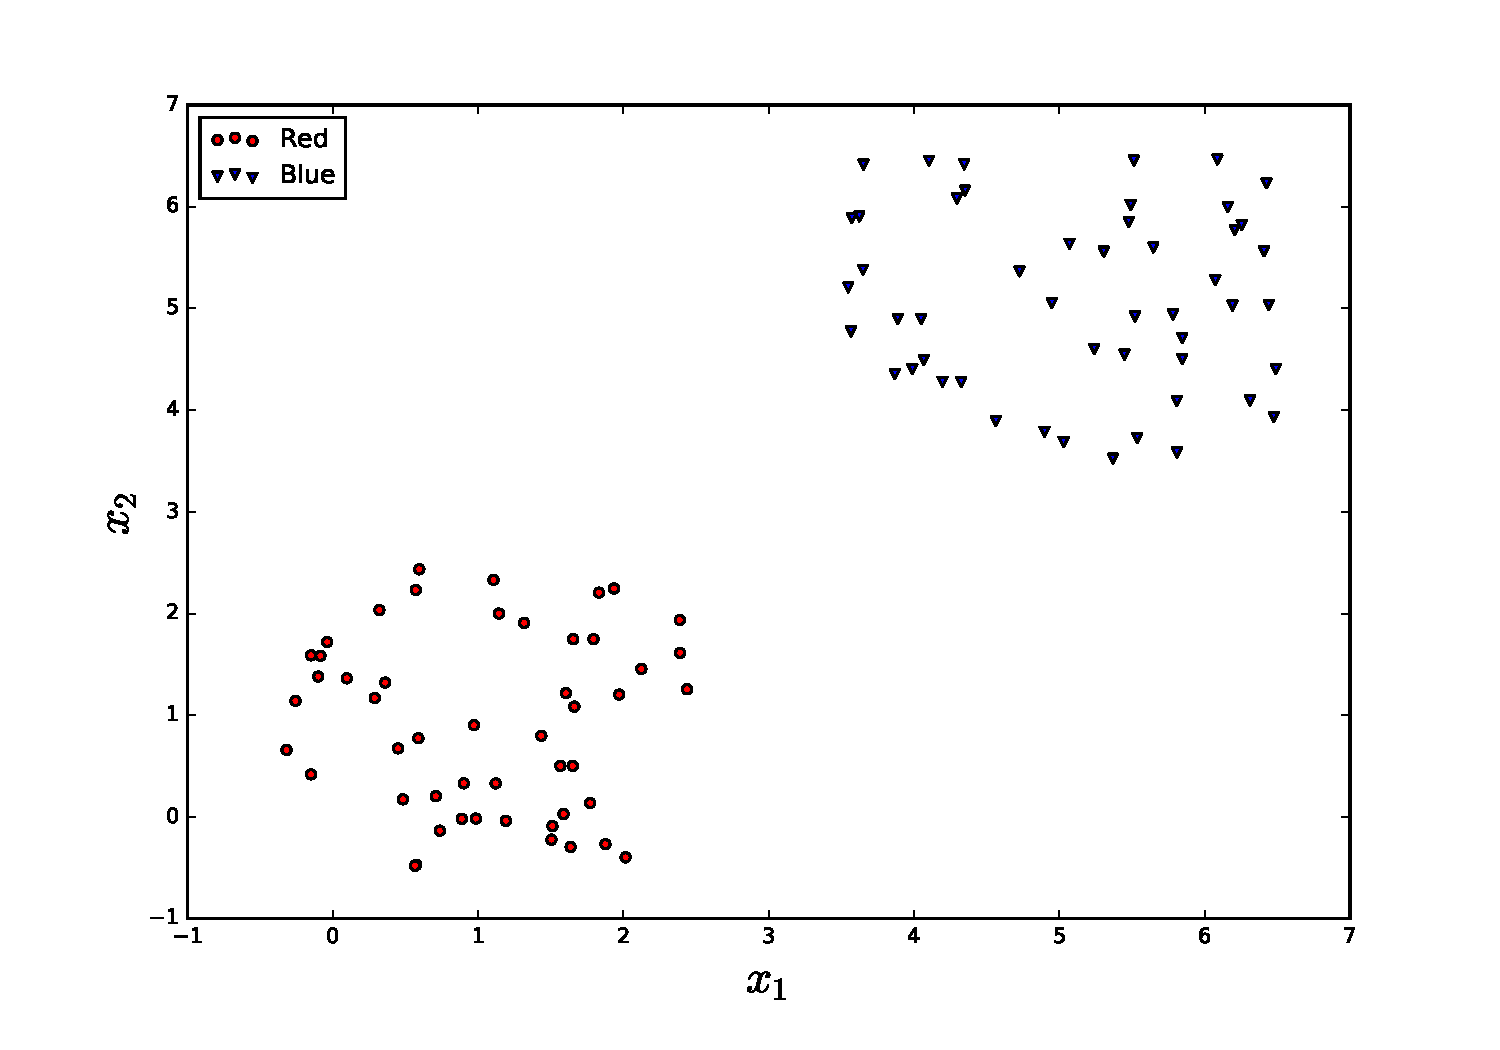
\includegraphics[width=\linewidth]{figures/twoClasses_separable.pdf}
  \end{subfigure} %
  \begin{subfigure}{0.49\textwidth}
    \centering
    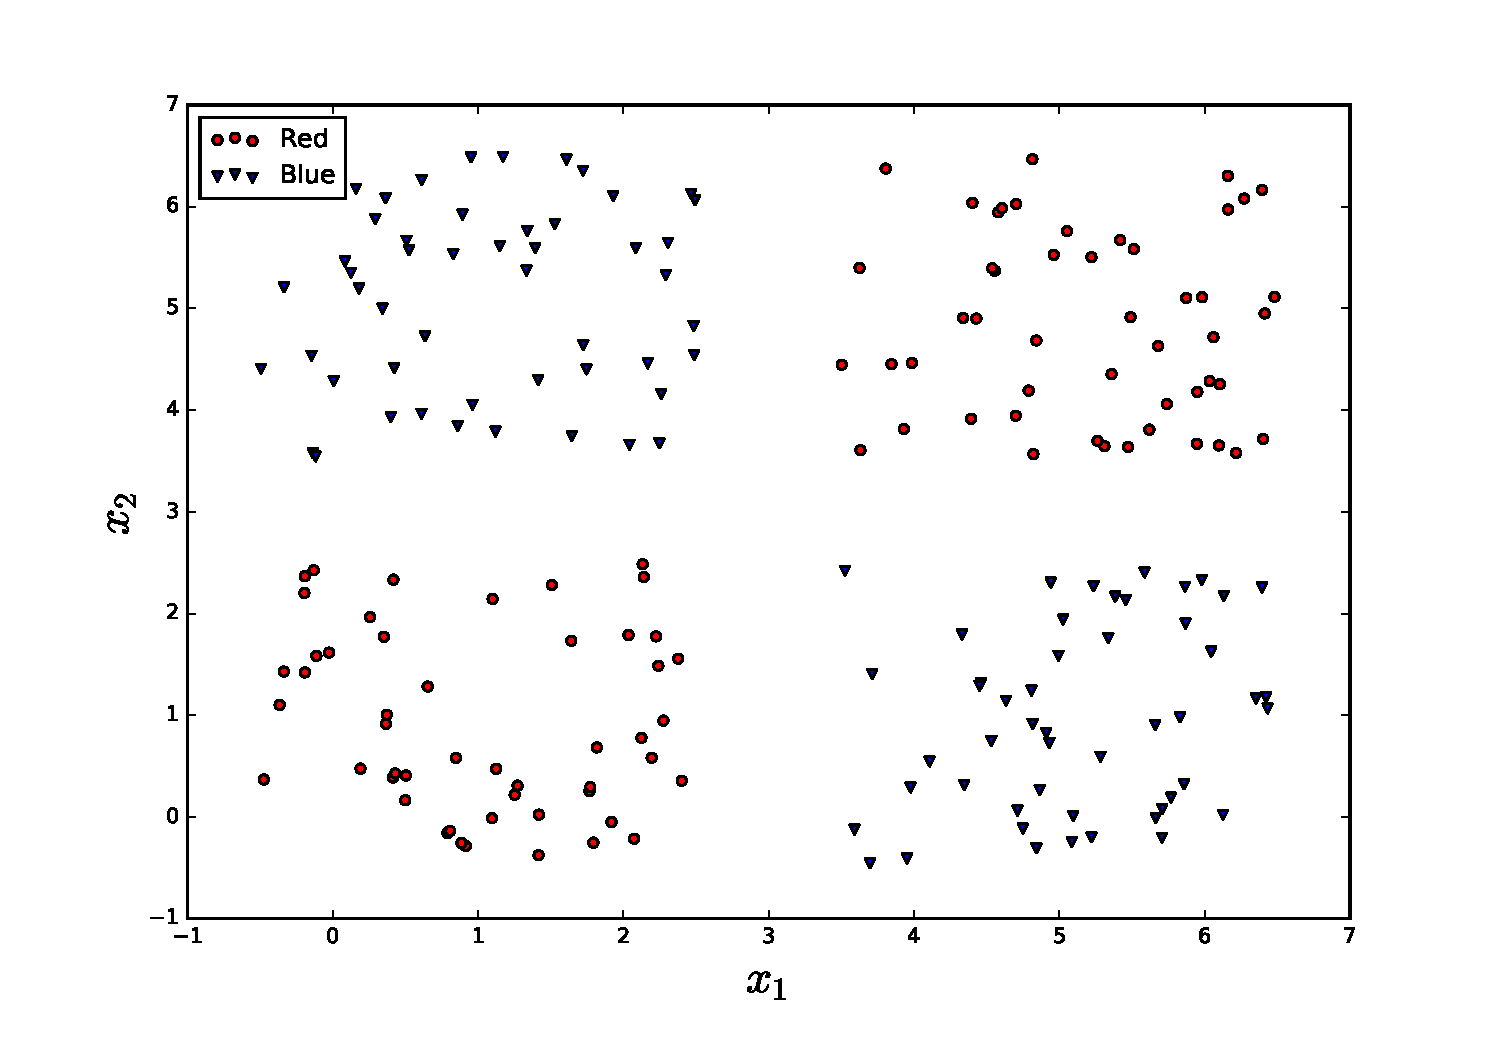
\includegraphics[width=\linewidth]{figures/twoClasses_non_separable.pdf}
  \end{subfigure}
  \caption{Two sets of data, one of which is linearly separable (Left) and the other is non linearly separable (Right). Linear separability means that a line can be found that can perfectly segregate the two classes into two sections. A diagonal, horizontal, or vertical line between the blue and red points can be drawn on the left that achieves that goal. However, on the right there is no one line that can be used to separate the red from blue points. This problem of finding a line of separation between two linearly separable data sets can be solved by using a binary classifier, the earliest example of which is the perceptron.}
  \label{fig:two_classes_example}
\end{figure}

 The perceptron was the first machine learning algorithm designed to solve binary classification in linearly separable conditions. Perceptrons were designed to mimic the McCollough-Pitts neuron model which relied on three main components: inputs, weights, and an activation function. In addition to these components, the perceptron had a learning rule that allowed it to learn when to and not to fire. Listing all the components of a perceptron:
\begin{itemize}
  \item \textbf{Inputs}: A dataset of $n$ dimensional points. Each input point $x$ consists of $n$ features such that each input point can be describes as $(x_1, x_2, \dots, x_n)$.
  \item \textbf{Weights}: $n$ weights described as $w_1, w_2, \dots, w_n$. These weights are randomly initialized.
  \item \textbf{Activation function}: a function on which the neuron decides to fire or not fire. The first one was the threshold (or step) function where the neuron fires if the weighted sum of inputs and weights is larger than threshold $\theta$, and doesn't fire otherwise.
  \item \textbf{Learning Rule}: A rule by which the weights change, described below.
\end{itemize}

% After being trained, the perceptron would fire to indicat that it has seen one class of data points (+1) and would not fire to indicate that it has seen the other class of data points (-1). 

A perceptron can be trained by passing to it each data point from the the dataset. In our example (Fig. \ref{fig:two_classes_example}), each data point would have a two-dimensional input consisting of the $x_1$ and $x_2$ values. Since we are working with two dimensions, the perceptron would have two weights $w_1$ and $w_2$. Every time the perceptron encounters a data point it tries to make a prediction by calculating the weighted sum of the inputs $S$  as $\sum_{i=1}^n w_ix_i$. If $S \geq \theta$ then the neuron fires, meaning it predicts the category to be $+1$. If $S < \theta$, the neuron doesn't fire, predicting the category to be $-1$. Given this determination, the perceptron evaluates its predicted output with the actual output of the data point, then manipulating its weights, completing the learning process of the perceptron on that data point. 

The learning process for input $x$, given a true label $\gamma$ and a threshold $\theta$ is summarized by the following updates:
\begin{align}
  S &= \sum_{i=1}^n w_ix_i > 0  \\
  \kappa &= \begin{cases} 
  \label{eq:piecewise_threshold_function}
    +1 \textrm{ if $S$} > \theta \\
    -1 \textrm{ otherwise} 
  \end{cases} \\
  w_{new} &= w_{old} + (\kappa - \gamma)x.
\end{align}

As can be seen from above, the perceptron learns by changing its weights, as this causes the same input to give a different $S$ which in turn could give a different predicted value $\kappa$. Following this learning rule, it can be proven that the perceptron model converges in finite time to a set of weights that result in a perfect classification for all data points in the dataset. A simple implementation of the perceptron was used to solve the sample datasets presented earlier (Fig \ref{fig:perceptron_solution}).

\begin{figure}[!h]
  \centering
  \begin{subfigure}{.49\textwidth}
    \centering
    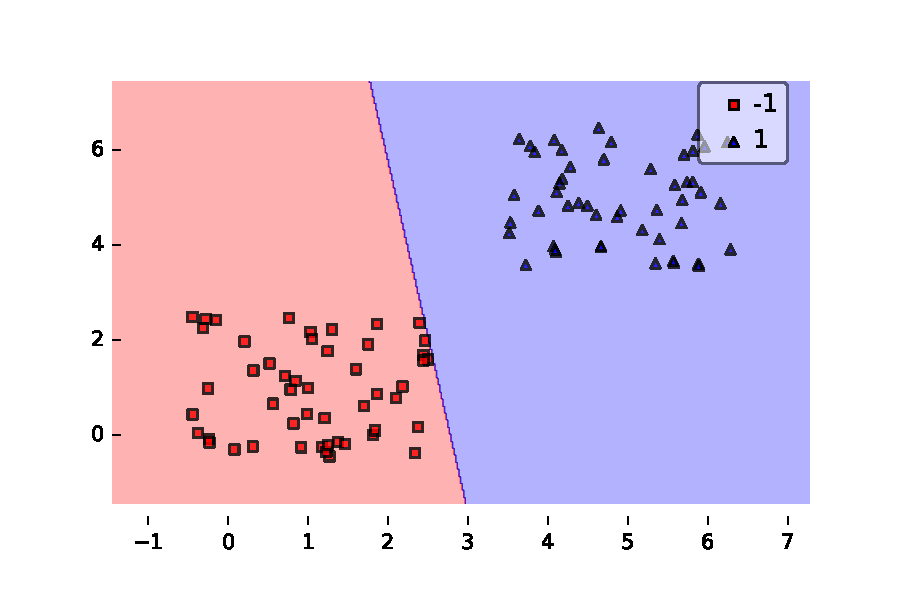
\includegraphics[width=\linewidth]{figures/perceptron_solvable.pdf}
  \end{subfigure} %
  \begin{subfigure}{0.49\textwidth}
    \centering
    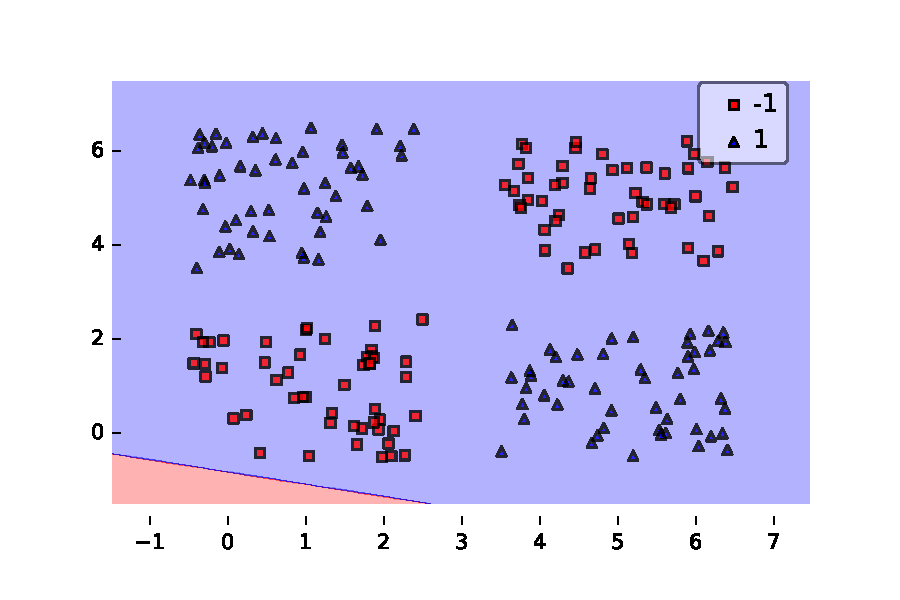
\includegraphics[width=\linewidth]{figures/perceptron_non_solvable.pdf}
  \end{subfigure}
  \caption{The perceptron model can be used to solve binary classification in linearly separable datasets as in the left image. After training, all points below the shown line of separation would be classified as -1, and all points above the line would be classified as +1. Seemingly, this behavior would correctly extrapolate to unseen data points from a similar distribution. In the case of non linearly separable datasets, the perceptron keeps adjusting its weights but never reaches a solution which correctly classifies all data inputs, meaning the model quits after a set limit of iterations through the dataset. This results in a having a line that clearly does not separate the two classes (Right).}
  \label{fig:perceptron_solution}
\end{figure}

The perceptron model did exceptionally well in solving such binary problems when it was introduced, but its lack of versatility when facing non linearly separable datasets resulted in an echoing cry of concern as to how realistic of a learner it could be. In fact, the scathing criticism that the perceptron model received lead to a 10-year hiatus in research on perceptrons \cite{minsky1969perceptrons}. Researchers who worked on the perceptron and neural network fields published under the umbrellas of  "adaptive signal processing", "pattern recognition", and "biological modeling" \cite{Yadav2015}. Slowly but surely, some loyalists to the neural machine learning perspective worked on enhancements to the perceptron model, leading to breakthroughs that skewed public opinion back in favor of what researchers now call neural networks: a group of perceptrons that are linked together to perform learning on datasets that one perceptron alone couldn't learn. 

\subsubsection{Neural Networks}
\label{sec:neural_networks}
Neural networks were first implemented by linking perceptrons together to attempt to solve problems that a single perceptron seemed unable to solve. While initial attempts did not indicate that this approach yielded a distinctly superior model, three major breakthroughs were integral to the uphill battle that neural network researchers had to fight in order to regain recognition in the machine learning field. The first breakthrough came when scientists put several neurons together in different topologies (Fig \ref{fig:perceptron_layers_example}), calling them a neural network. In a neural network, layers can be defined as a collection of nodes that are fed data from a previous layer, perform a calculation on this data, and pass it to another layer or as a final result.  Although the neural network could approximate more functions, there was no clear way to tune the learning rule from one layer to another. This is when the second and third important ideas came about. The second breakthrough was a realization that choosing a different, continuous activation function (as opposed to the discrete step function) could mean that a derivative could be taken (Fig. \ref{fig:activation_functions}). The third was a method by which the chain rule (from calculus) can be employed on the these derivatives that allows error calculations to be passed down from layer to layer reliably, a method called Back Propagation (Fig. \ref{fig:back_propagation}). Together, these breakthroughs caused a resurgence in the field of neural networks which used perceptrons as their building block. When the activation function changed from a step function, the field moved away from the perceptron naming convention, and used the term \textit{learning units} instead (Fig. \ref{fig:activation_functions}, \ref{fig:perceptron_layers_example}). The name change is also because the learning rule changes with the change of the activation function, which moves the learning unit further away from the initial conceptualization of the perceptron model.


\begin{figure}[!h]
  \centering
  \begin{subfigure}{.49\textwidth}
        \centering
        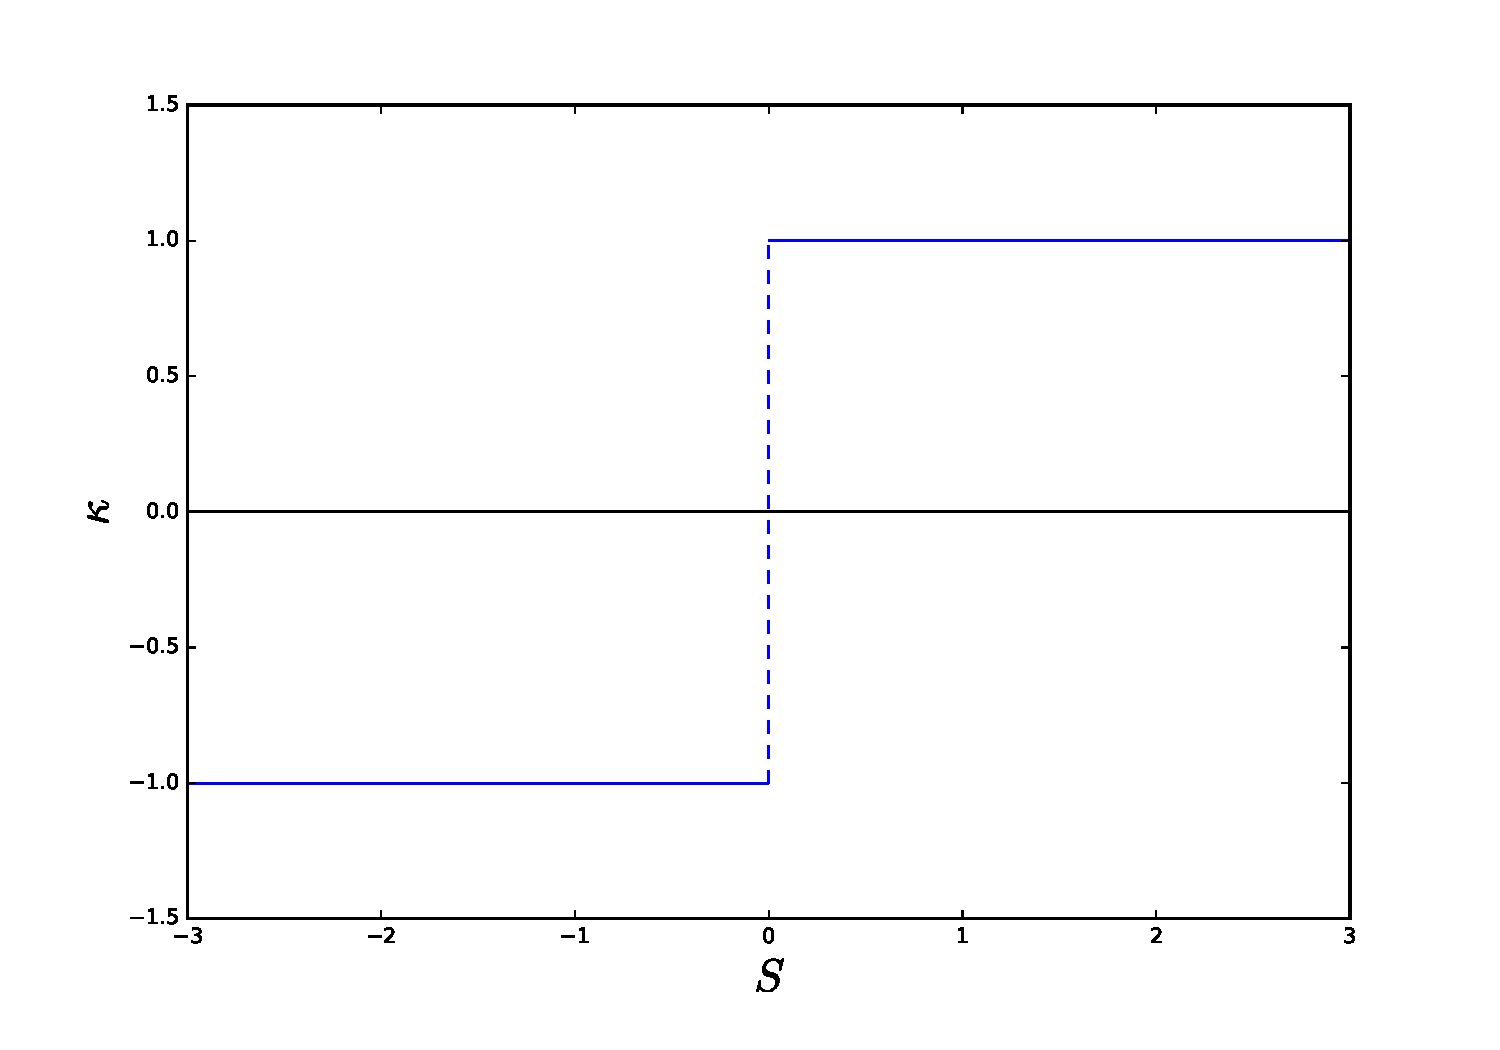
\includegraphics[width=\linewidth]{figures/stepfunction.pdf}
    \end{subfigure} %
    \begin{subfigure}{0.49\textwidth}
        \centering
        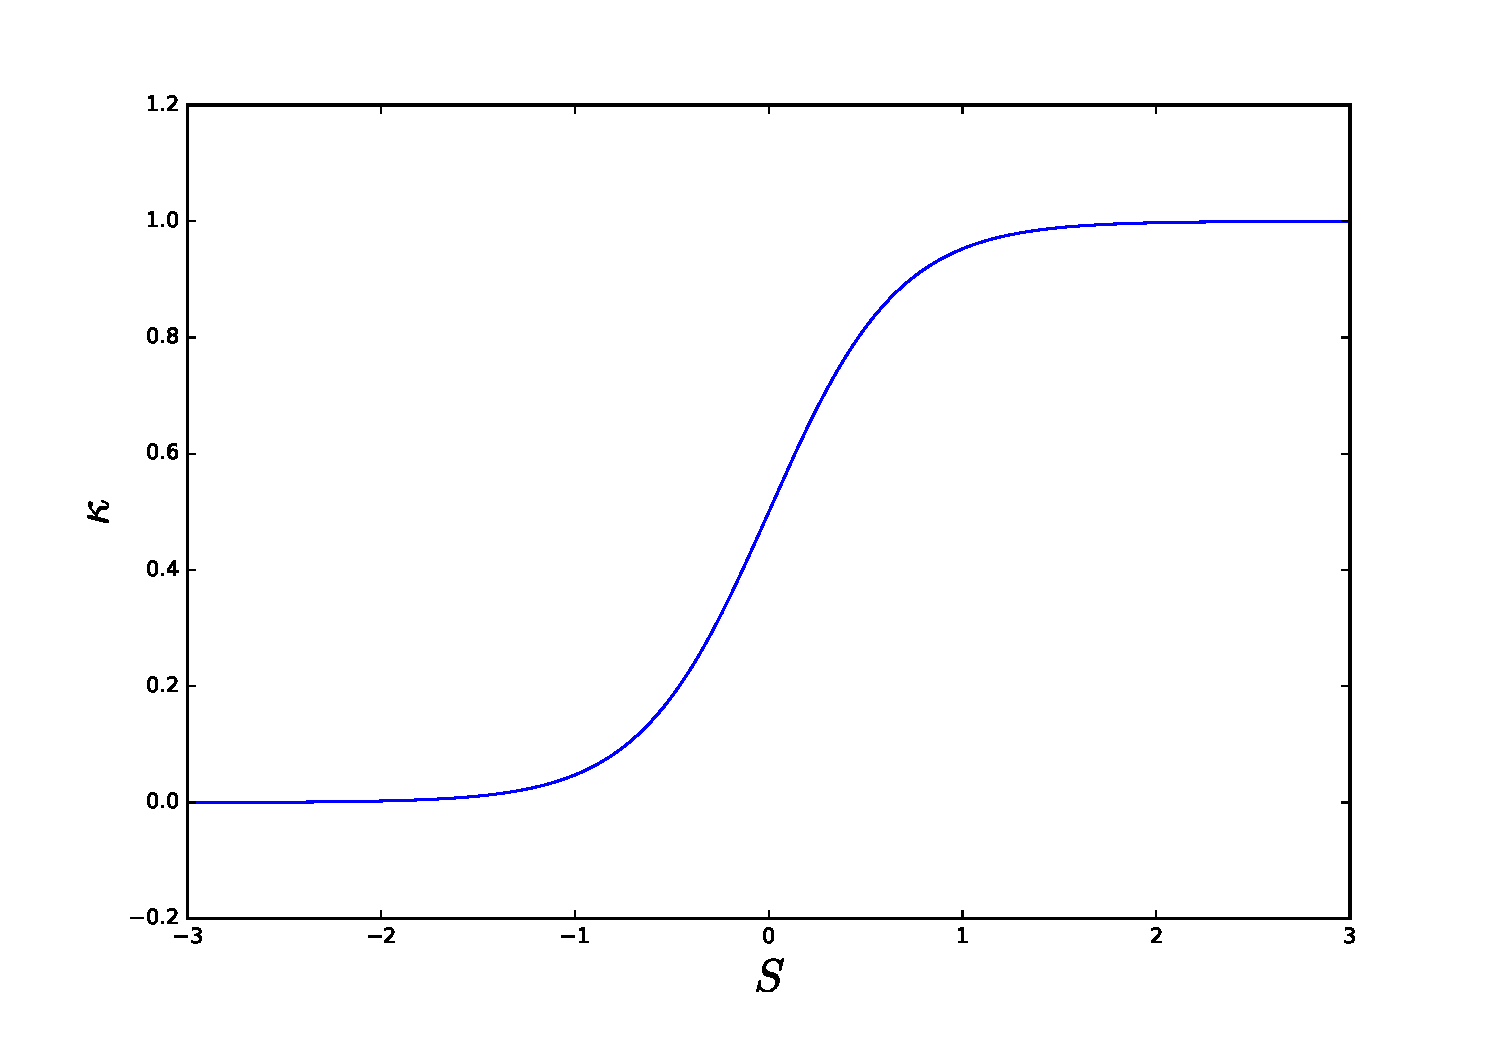
\includegraphics[width=\linewidth]{figures/logisticfunction.pdf}
    \end{subfigure}
  \caption{Different activation functions can be applied to the perceptron model. The simplest and earliest activation function is the step function (Left) which outputs either a $+1$ or $-1$. A disadvantage of the step function is that small changes in the weighted sum ($S$) could cause a large change in the output ($\kappa$). This is solved by the sigmoid activation function (right) which gives a output (between $0$ and $+1$) that is proportional to $\S$ within a given range. When a perceptron implements a sigmoid activation unit, it is referred to as a sigmoid learning unit.}
  \label{fig:activation_functions}
\end{figure}



% Credit to http://tex.stackexchange.com/questions/140782/drawing-a-neural-network-architecture
\begin{figure}[!h]
  \centering
  \begin{subfigure}{0.20\linewidth}
    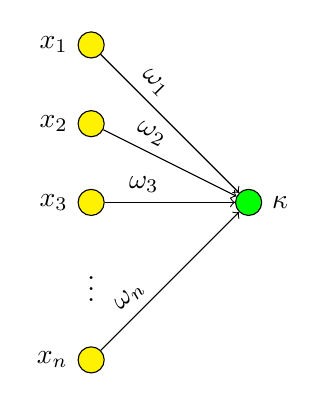
\begin{tikzpicture}
    [   cnode/.style={draw=black,fill=#1,minimum width=3mm,circle},
    ]
        \node[cnode=green,label=0:$\kappa$] (s) at (2,-3) {};
        \node at (0,-4) {$\vdots$};
        % \node at (3,-4) {$\vdots$};
        \foreach \x in {1,...,4}
        {   \pgfmathparse{\x<4 ? \x : "n"}
            \node[cnode=yellow,label=180:$x_{\pgfmathresult}$] (x-\x) at (0,{-\x-div(\x,4)}) {};
            \draw[->] (x-\x) -- node[above,sloped,pos=0.3] {$\omega_{\pgfmathresult}$} (s);
        }
    \end{tikzpicture}
  \end{subfigure}  
  \begin{subfigure}{0.30\linewidth}
  % middle figure
  \centering
  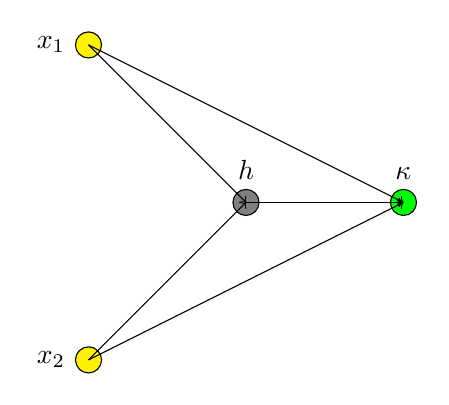
\begin{tikzpicture}
    [   cnode/.style={draw=black,fill=#1,minimum width=3mm,circle},
    ]
        % drwaw the nodes
        \node[cnode=yellow, label=180:$x_1$] (s) at (0,-2) {};
        \node[cnode=yellow, label=180:$x_2$] (s) at (0,-6) {};
        \node[cnode=gray, label=90:$h$] (s) at (2,-4) {};
        \node[cnode=green,label=90:$\kappa$] (s) at (4,-4) {};

        % draw the lines
        \draw[->] (0,-2) -- (2,-4);
        \draw[->] (0,-6) -- (2,-4);
        \draw[->] (0,-2) -- (4,-4);
        \draw[->] (0,-6) -- (4,-4);
        \draw[->] (2,-4) -- (4,-4);
    \end{tikzpicture}
  \end{subfigure}  
  \begin{subfigure}{0.40\linewidth}
    \centering
    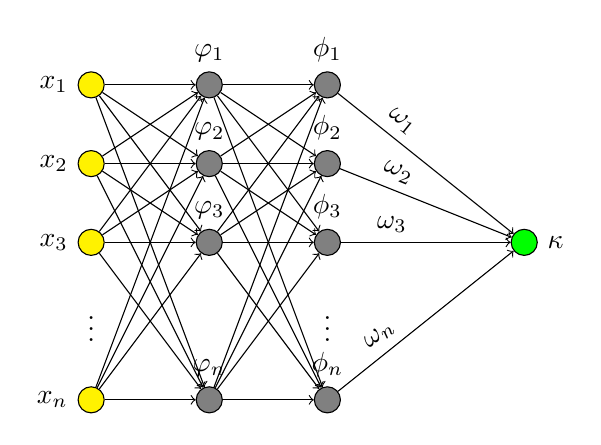
\begin{tikzpicture}
    [   cnode/.style={draw=black,fill=#1,minimum width=3mm,circle},
    ]
        \node[cnode=green,label=0:$\kappa$] (s) at (5.5,-3) {};
        \node at (0,-4) {$\vdots$};
        \node at (3,-4) {$\vdots$};
        \foreach \x in {1,...,4}
        {   \pgfmathparse{\x<4 ? \x : "n"}
            \node[cnode=yellow,label=180:$x_{\pgfmathresult}$] (x-\x) at (0,{-\x-div(\x,4)}) {};
            \node[cnode=gray,label=90:$\varphi_{\pgfmathresult}$] (l-\x) at (1.5,{-\x-div(\x,4)}) {};
            \node[cnode=gray,label=90:$\phi_{\pgfmathresult}$] (p-\x) at (3,{-\x-div(\x,4)}) {};
            \draw[->] (p-\x) -- node[above,sloped,pos=0.3] {$\omega_{\pgfmathresult}$} (s);
        }
        \foreach \x in {1,...,4}
        {   \foreach \y in {1,...,4}
            {   
              \draw[->] (x-\x) -- (l-\y);
              \draw[->] (l-\x) -- (p-\y);
            }
        }
    \end{tikzpicture}
  \end{subfigure}
  \caption{Perceptrons linked in networks with different topologies. Yellow represents input notes, gray represents hidden nodes, and green represents output nodes. The left network contains only one layer, the input layer, with its associated weights that feed into the output layer. This network essentially simulates a computation that is equivalent to the perceptron model. The center network contains a hidden layer composed of simply 1 node. This network can solve the XOR problem, and is able to solve the linearly inseparable dataset in Fig \ref{fig:two_classes_example}. The more nodes added to the hidden layer and the more hidden layers there are, the more communication happens between the nodes in the previous layer, and therefore the higher the abstraction. The network on the right is a more dense network with two hidden layers and many more hidden nodes.}
  \label{fig:perceptron_layers_example}
\end{figure}

A common continuous activation function for learning units is the sigmoid learning unit. Instead of the stepwise function in equation \ref{eq:piecewise_threshold_function}, the output function becomes
\begin{align}
  \kappa &= \sigma(S) = \frac{1}{1+e^{-S}}
\end{align}
which is bounded by 0 and 1. This function is popular because its derivative is rather simple to compute and leads directly into the theory of back propagation. When the sigmoid function is used, the learning rule becomes a minimization of an error term using gradient descent. For a data point with target classification $\lambda$ and predicted classification $\kappa$, the error term is described as
$$ \epsilon = (\lambda- \kappa)^2 $$
and is called MSE and is derived in \ref{sec:regression_supervised_learning}. Gradient descent is an iterative approach to finding the maximum or minimum of a continuous function by using its derivative (Fig. \ref{fig:gradient_descent}).


For example, if a learning unit predicts an output of $\kappa$ with an error $\epsilon$ and it has two learning units feeding it


\begin{align*}
  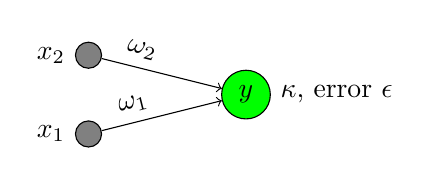
\begin{tikzpicture}
    [   cnode/.style={draw=black,fill=#1,minimum width=3mm,circle},
    ]
        \node[cnode=green,label=0:{$\kappa$, error $\epsilon$}] (s) at (2,-1.5) {$y$};
        \foreach \x in {1,...,2}
        {   \pgfmathparse{\x}
            \node[cnode=gray,label=180:$x_{\pgfmathresult}$] (x-\x) at (0,\x-3) {};
            \draw[->] (x-\x) -- node[above,sloped,pos=0.3] {$\omega_{\pgfmathresult}$} (s);
        }
  \end{tikzpicture}
\end{align*}
and keeping in mind that $\kappa$ is $\sigma(S) = \frac{1}{1+e^{-S}} = \frac{1}{1+e^{-\sum_{i=1}^n w_ix_i}}$ then the error can be expressed as 
$$ \epsilon = (\lambda - \kappa)^2  =  (\lambda - \sigma(S))^2$$ 
or in our example  
$$ \epsilon = \Big(\lambda - \frac{1}{1+e^{-w_1x_1-w_2x_2}}\Big)^2$$
Using gradient descent, minimizing $\epsilon$ with respect to node $x_i$ requires us to change $w_i$ by the negative of its gradient. This gradient is 

\begin{align}
  \frac{\partial MSE}{\partial w_i} = \frac{\partial(\lambda - \sigma(S))^2}{\partial w_i}  = \frac{\partial\sigma(S)}{\partial w_i}2(\lambda - \sigma(S))
  \label{eq:gradient_descent_on_sigma}
\end{align}

because $\sigma(S)$ is the only function of $w_i$. This is where having an activation function that can be easily differentiated is advantageous. For the sigma function, the derivative evaluates to
\begin{align}
\frac{\partial\sigma(S)}{\partial w_i} =  \frac{\partial \frac{1}{1+e^{-\sum_{j=1}^n w_jx_j}}}{\partial w_i} = \frac{x_ie^{-\sum_{j=1}^n w_jx_j}}{\Big({1+e^{-\sum_{j=1}^n w_jx_j}}\Big)^2} = \sigma(S)^\prime.
\label{eq:sigma_derivative}
\end{align}
The last step is carried for notational simplicity. Combining equations \ref{eq:gradient_descent_on_sigma} and \ref{eq:sigma_derivative}, we find that the weight of the $i$th node $w_i$ must be changed by the negative of the gradient

\begin{align*}
  2\sigma(S)^\prime(\lambda - \sigma(S))
\end{align*}
which leads to a weight update rule of 
\begin{align}
  w_{i_{t+1}} = w_{i_t} - 2\sigma(S)^\prime(\lambda - \sigma(S))
  \label{eq:update_rule_for_sigma}
\end{align}

In this way, the error that is produced at the top layer, where the final classification decision is contrasted with the desired decision, trickles down to all lower layers, with each node changing its weights according to the error of the upper node. Back propagation is worked on out example above in Figure \ref{fig:back_propagation}.


\begin{figure}[!h]
  \begin{subfigure}{0.45\linewidth}
    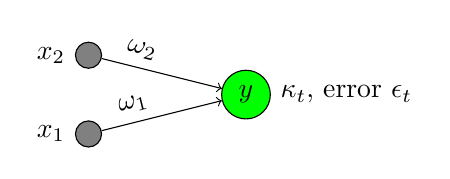
\begin{tikzpicture}
      [   cnode/.style={draw=black,fill=#1,minimum width=3mm,circle},
      ]
          \node[cnode=green,label=0:{$\kappa_t$, error $\epsilon_t$}] (s) at (2,-1.5) {$y$};
          \foreach \x in {1,...,2}
          {   \pgfmathparse{\x}
              \node[cnode=gray,label=180:$x_{\pgfmathresult}$] (x-\x) at (0,\x-3) {};
              \draw[->] (x-\x) -- node[above,sloped,pos=0.3] {$\omega_{\pgfmathresult}$} (s);
          }
    \end{tikzpicture}
    \caption{at time $t$}
  \end{subfigure}
  \begin{subfigure}{0.45\linewidth}
    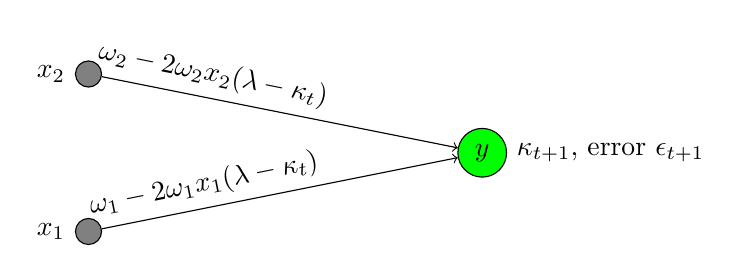
\begin{tikzpicture}
      [   cnode/.style={draw=black,fill=#1,minimum width=3mm,circle},
      ]
          \node[cnode=green,label=0:{$\kappa_{t+1}$, error $\epsilon_{t+1}$}] (s) at (5,3) {$y$};
          \foreach \x in {1,...,2}
          {   \pgfmathparse{\x}
              % z=\x-1
              \node[cnode=gray,label=180:$x_{\pgfmathresult}$] (x-\x) at ($(0,0)+ (0, {\x*2}) $) {};
              \draw[->] (x-\x) -- node[above,sloped,pos=0.3] {$\omega_{\pgfmathresult} - 2\omega_{\pgfmathresult}x_{\pgfmathresult}(\lambda - \kappa_t)$} (s);
          }
    \end{tikzpicture}
    \caption{at time $t+1$}
  \end{subfigure}
  \caption{Back propagation works by minimizing the error function using gradient descent. In this case, the error function is the MSE, and its partial derivative with respect to each weight from the $i$th node in the previous layer is $2w_ix_i(\lambda - \kappa_t$ where $\lambda$ is the desired outcome and $\kappa_t$ is the predicted outcome at iteration $t$. In each iteration, applying gradient descent results in a move towards the opposite of the gradient, meaning partial derivative of the error with respect to that weight is negated from the weight (right). This method is guaranteed to converge, however slowly, over well defined continuous activation functions, an example of which is the sigmoid function (Fig. \ref{fig:activation_functions}).}
  \label{fig:back_propagation}
\end{figure}

Some of these networks, if constructed properly, can solve linearly inseparable problems.
%TODO: Could talk about how to find if a datset is linearly separable. Could we use Perceptrons to do it?















\subsubsection{Decision Trees}
\label{sec:decision_trees}
A completely different approach to label classification is that of using decision trees to find the features that are most likely to hint at a correct approach towards finding a solution. For example, consider a problem where both the input and the output of the data is categorical. One such dataset is the swimming pool and weather dataset, in which each data point is a weather description of a day and whether or not the tennis court was open on that day (Table \ref{table:categorial_examples_weather}). In this dataset there are several weather-related features such as \textit{Outlook, Temperature, Humidity,} and \textit{Wind}. The \textit{Outlook} feature could contain categories such as sunny, overcast, or rainy; the \textit{Temperature} feature could include categories such as hot or cold; the wind category could include Strong or Weak. All these features contain values from finite set of possibilities. 

\begin{table}
\begin{center}
     \begin{tabular}{||c c c c c c||} 
    \hline
     Day & Outlook & Temperature & Humidity & Wind & Play \\ [0.5ex] 
    \hline\hline
     D1 & Sunny & Hot & High & Weak  & No\\ 
    \hline
     D2 & Sunny & Hot & High & Strong  & No\\ 
    \hline
     D3 & Overcast & Hot & High & Weak  & Yes\\ 
    \hline
     D4 & Rainy & Mild & High & Weak  & Yes\\ 
    \hline
     D5 & Rainy & Cool & Normal & Weak  & Yes\\ 
    \hline
     D6 & Rainy & Cool & Normal & Strong  & No\\ 
    \hline
     D7 & Overcast & Cool & Normal & Strong  & Yes\\ 
    \hline
     D8 & Sunny & Mild & High & Weak  & No\\ 
    \hline
     D9 & Sunny & Cool & Normal & Weak  & Yes\\ 
    \hline
     D10 & Rainy & Mild & Normal & Weak  & Yes\\ 
    \hline
     D11 & Sunny & Mild & Normal & Strong  & Yes\\ 
    \hline
     D12 & Overcast & Mild & High & Strong  & Yes\\ 
    \hline
     D13 & Overcast & Hot & Normal & Weak  & Yes\\ 
    \hline
     D14 & Rainy & Mild & High & Strong & No\\  [1ex]
    \hline
  \end{tabular}
\end{center}
\caption{Weather and Tennis court dataset example \cite{mitchell1997machine}. All features are categorical, meaning the values of the features are from a finite, relatively small set of possibilities. The values can not be numerically represented in a formula or compared, nor do they represent values on a range.}
\label{table:categorial_examples_weather}
\end{table}

Through a simple observation at the table, we can perhaps device our own conditions for when the tennis court is open.
\begin{align*}
    \textrm{If outlook}&=\textrm{sunny } \wedge \textrm{ humidity = high, then Yes} \\
    \textrm{If outlook}&= \textrm{rainy } \wedge \textrm{ wind = Strong , then Yes} \\
    \textrm{Otherwise, No}
\end{align*}

Although this might be a good rule to follow, it might not generalize well to the rest of the dataset, and inspecting the entire dataset by eye becomes unfeasible beyond $~20$ data points. This is where the decision tree algorithm comes in, offering an automated method of finding such rules by which we can separate data points into \textit{Yes} and \textit{No} piles. In the simplest decision tree algorithm algorithm, the data points are iteratively separated by the feature that splits the data most evenly (or produces the most homogeneity within a feature split). For example, if we were to take the \textit{Wind} feature and split the Strong and Weak wind conditions into two piles, and observe how mixed or 'pure' the piles are, we would get a sense of how well the \textit{Wind} feature can split up our decision (Fig \ref{fig:split_on_wind}).

\begin{figure}
  \centering
    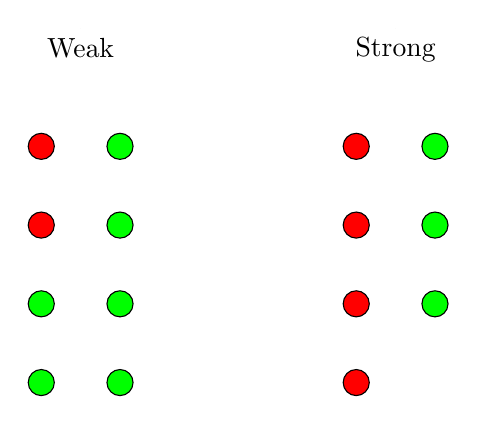
\begin{tikzpicture}
      [   cnode/.style={draw=black,fill=#1,minimum width=3mm,circle},
      ]
          \filldraw[black] (0.5, 1.5) circle (0pt) node[anchor=north] {Weak};
          \node[cnode=red] (s) at (0,0) {};
          \node[cnode=red] (s) at (0,-1) {};
          \node[cnode=green] (s) at (0,-2) {};
          \node[cnode=green] (s) at (0,-3) {};
          \node[cnode=green] (s) at (1,0) {};
          \node[cnode=green] (s) at (1,-1) {};
          \node[cnode=green] (s) at (1,-2) {};
          \node[cnode=green] (s) at (1,-3) {};

          \filldraw[black] (4.5, 1.5) circle (0pt) node[anchor=north] {Strong};
          \node[cnode=red] (s) at (4,0) {};
          \node[cnode=red] (s) at (4,-1) {};
          \node[cnode=red] (s) at (4,-2) {};
          \node[cnode=red] (s) at (4,-3) {};
          \node[cnode=green] (s) at (5,0) {};
          \node[cnode=green] (s) at (5,-1) {};
          \node[cnode=green] (s) at (5,-2) {};
    \end{tikzpicture}
    \caption{The decisions to play or not play tennis when the decision is split on wind conditions. Red balls represent No and green balls represent Yes. As we can tell from this graph, splitting on the Wind feature does not provide a homogeneous set (both sides of the split are not purely green or purely red). This means that we can't conclude that whenever the wind is strong tennis can not be played, vise versa. However, It seems that the split caused us to see a relationship between wind conditions and playing tennis, since when the wind was weak most decisions were to play tennis, while when it was wind most decisions were not to play tennis.}
    \label{fig:split_on_wind}
\end{figure}

This idea of purity or homogeneity is represented in the mathematical formula for entropy (taken from the Information Theory field) as follow

\begin{align}
Entropy = \sum_{i=1}^n p_i log_n(p_i)
\end{align}
where $n$ is the number of decisions possible and $p_i$ is the fraction of the decisions that were in the $i$th decision. This definition can be used to calculate the entropy in each of our splits. In our \textit{Wind} feature split example, we can measure the entropy in our Strong and Weak split. In each split our decision possibilities were two (Yes or No); our Strong split had 0.57 fraction No and 0.43 Yes; our Weak split had 0.25 fraction No and 0.75 fraction Yes. So the entropy calculation for the Strong split becomes

$$ - \Big(  0.57*log_2(0.57) + 0.43*log_2(0.43)  \Big) = 0.985$$
and for the Weak split the entropy is
$$ - \Big(  0.25*log_2(.25) + .75*log_2(.75)   \Big) = 0.811 \text{ .}$$

Figure \ref{fig:entropy_two_decisions} provides some intuition as to what entropy measures. Using this metric, we can devise an algorithm to iteratively pick the feature that that contains the least entropy when splitting the data upon. However, a more concrete way of using Entropy is measuring \textit{Information Gain} on each split. Information gain is a measure of how much entropy is lost through a transition. The equation that describes information gain is

\begin{align}
\textit{Information Gain} = Entropy(S) - \sum_{v\in Values(F)} \frac{|T_v|}{|T|}Entropy(T_v)
\end{align}
where F is the feature we are splitting on, $|T_v|$ is the number of decisions with split value $v$, $|T|$ the number of total decisions, and $Entropy(T_v)$ is the measure of entropy on the decisions with split value $v$. In our wind example, the entropy of the original system (without any splitting on any feature) is $-\big(\frac{5}{14}*log_2(5/14) + \frac{9}{14}*log_2(9/14) \big) =  0.94$. Since we had two splits on \textit{Wind}, let $v_1$ be the Strong split and $v_2$ be the Weak split then

\begin{align*}
  \textit{Information Gain(Wind)} &= Entropy(Original) - \frac{|T_{v_1}|}{|T|}Entropy(T_{v_1}) - \frac{|T_{v_2}|}{|T|}Entropy(T_{v_2}) \\
   &= 0.94 - \frac{6}{14}0.985 - \frac{8}{14}0.811 \\
   &= 0.054
\end{align*}

In this manner, we can measure the information gain on splitting on each available feature, and choose the feature that results in the highest information gain split. This would give us two to three bins, on which we iteratively carry out this process again choosing another feature and so on. A decision tree is the amalgamation of all these decisions, put in a concise diagram (Fig. \ref{fig:decision_tree_for_tennis}). This algorithm has the distinct advantage of being able to display its reasoning efficiently, a feat that some machine learning algorithms can not accomplish.

\begin{figure}
  \centering
  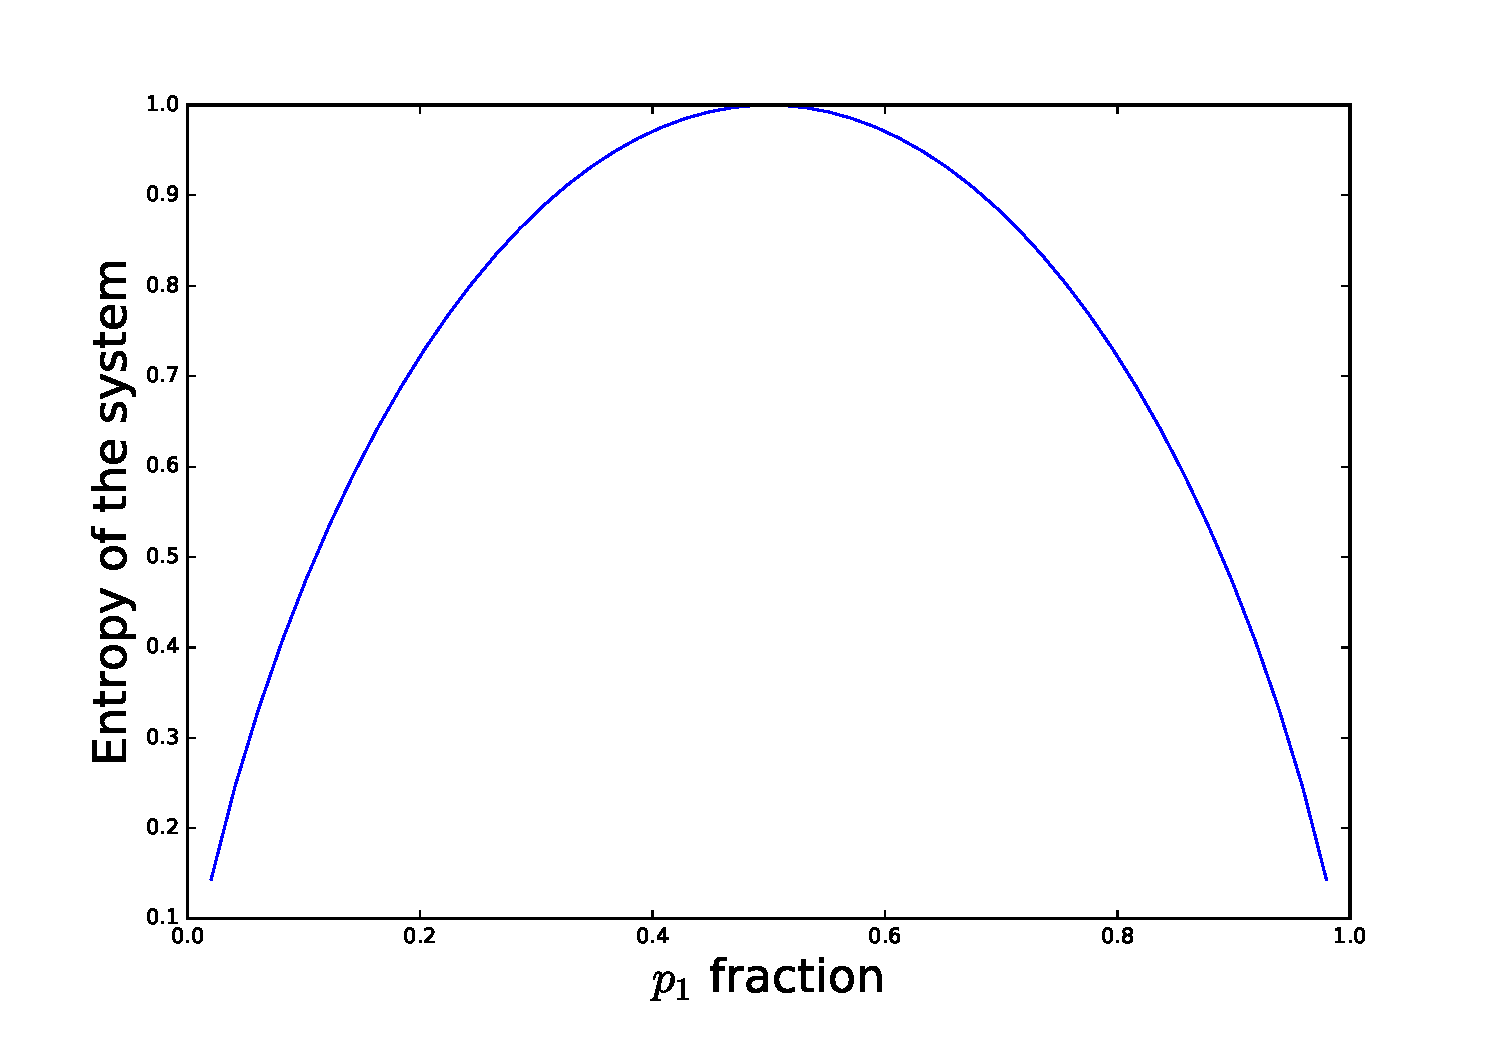
\includegraphics[width=0.7\linewidth]{figures/entropy_fig.pdf}
  \caption{The entropy of a system with two decisions each of which have a fraction $p_1$ and $p_2$ (fraction $p_2$ is not shown here because it is simply $1-p_1$). When the system has both fractions in equal proportions, it is perfectly heterogeneous, so it has the highest entropy measure of $1$. On the other end, when one fraction dominates the system, the entropy goes to $0$. In this way, entropy measures how "polluted" or pure a system is, giving a higher score to disorganized, polluted systems, and a lower score to homogeneous, pure systems.}
  \label{fig:entropy_two_decisions}
\end{figure}

\begin{figure}
\centering
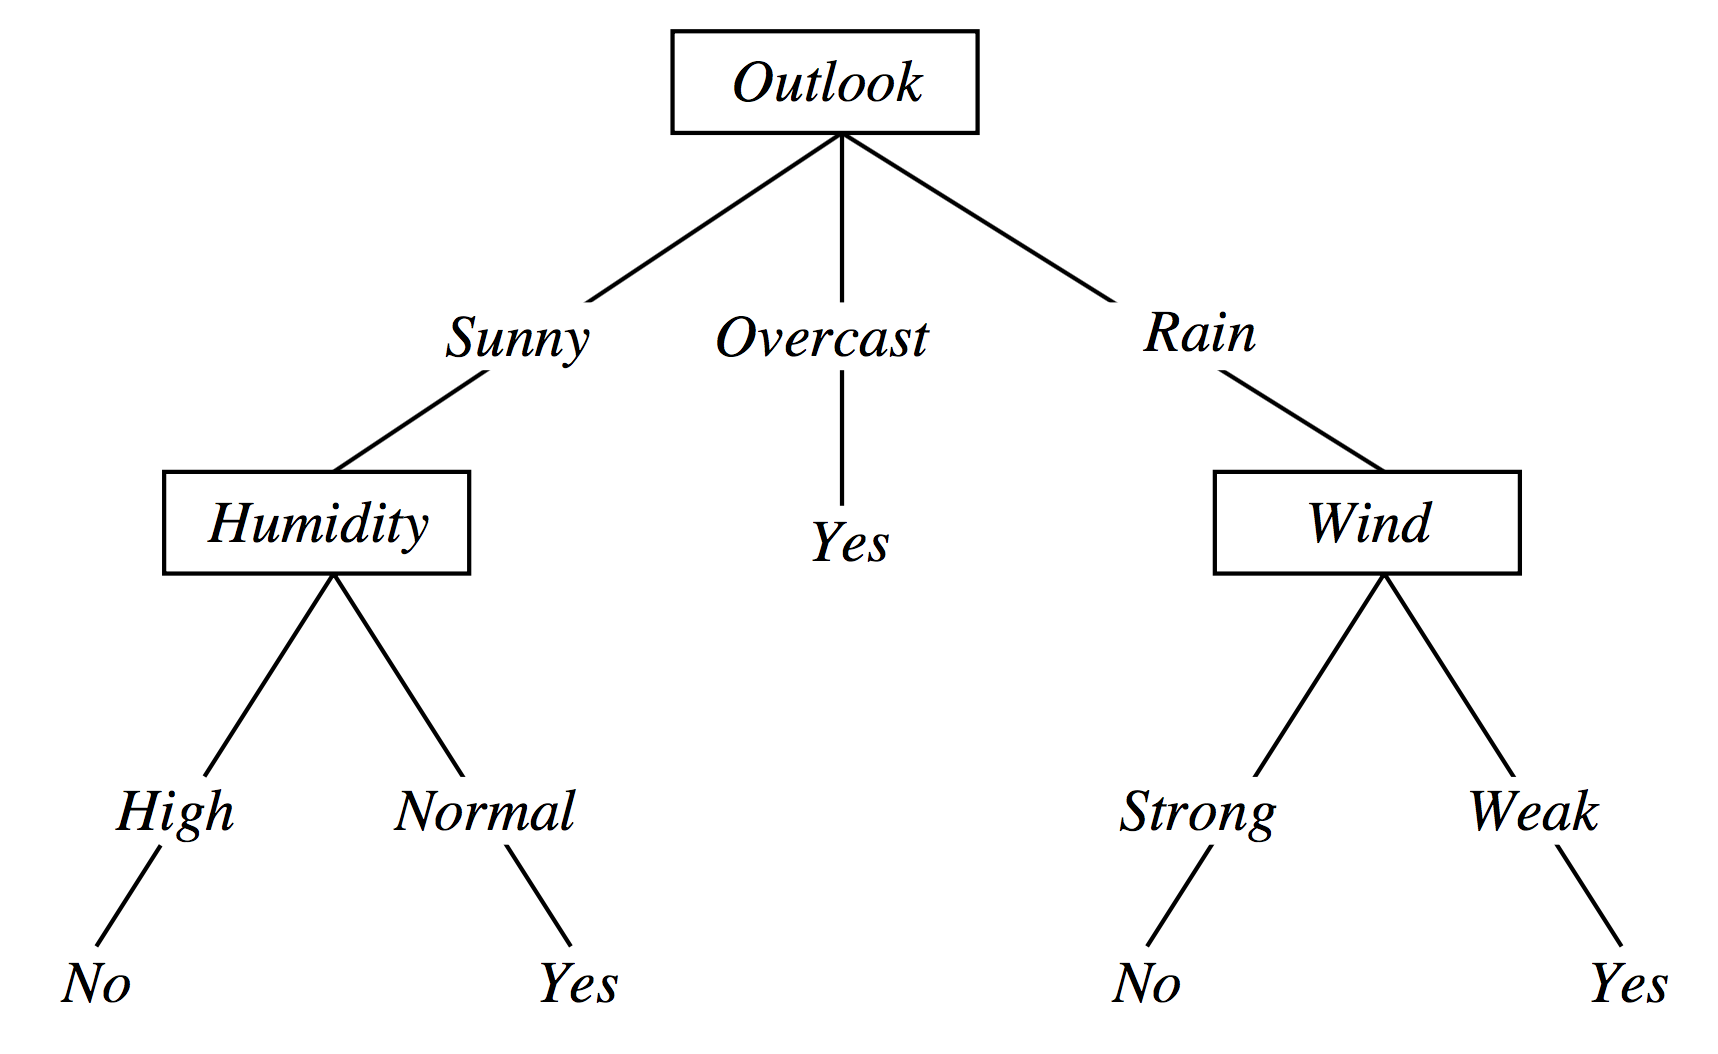
\includegraphics[width=0.7\linewidth]{figures/tennis_decision_tree_mitchel.png}
\caption{A decision tree that can be generated by iterating over the tennis-weather dataset using the information gain equation. This is taken from Michel's book on Machine Learning \cite{mitchell1997machine}.}
\label{fig:decision_tree_for_tennis}
\end{figure}



\subsubsection{Regression Prediction}
\label{sec:regression_supervised_learning}
For cases when the desired output of a function is a number on a meaningful range, label classification is not possible. This is because a supervised label classification problem deals with \textit{choosing} the best label out of a given set, and not generating a label out of the given data. This is where regression prediction comes into play. For functions whose output is a continuous range of numbers, one can not possibly assign a label to each possible output. And even if each output is assignable, there is rarely a dataset big enough to cover possible mappings to each such label.

For example, given an input set of ${1,2,3,4,5,6,7}$ and an output set ${1,4,9,14,25,36,49}$, a good---and almost any---supervised learning algorithm should approximate the function $f(x^2)$. However, such a function would have rely on regression learning, and not label classification. To show this, let's delve into a thinking exercise. Say we make a training set for the function $f(x) = x^2$ consisting of input that is all the integers from one to one million and output that is the square of all these input numbers. If we are to use label classification, then we would train the algorithm to map each number to its square label. The first problem arises on the first step of learning, especially in the Decision Tree technique. Because each input is looked at as a categorical input, an input of one (1) will be converted to a label. Since each data point has its own label, the information gain will be maximized and the entropy loss will be minimized when the input is split into one million branches on the first level of the tree. At that point, the function mapping is resolved by simply going through one level. However, this leads to the second problem, which arises when feeding in new test data that the classifier was not trained on. Because the classifier only has access to labels that it trained on, any number other than an integer from one to million will have to map to an already known label from the squares of the integers from one to one million. For example, an input of $1.76$ will map to either $1$ ($1^2=1$) or $4$ ($2^2 = 4$), meaning this incurs an accuracy cost. This cost might not be a big problem for the purposes of the algorithm, but the real problem arises when we try to predict the mapping of a number outside the range of our training dataset: numbers below 0 and those above one million. The nearest value for all numbers below 0 is $1$, so all the numbers below 0 will be mapped to the label of $0$, while all the numbers above one million will be mapped to the label of one million (Fig \ref{fig:decision_tree_regression_and_classification}).

\begin{figure}[!h]
  \centering
    \begin{subfigure}{0.49\textwidth}
        \centering
        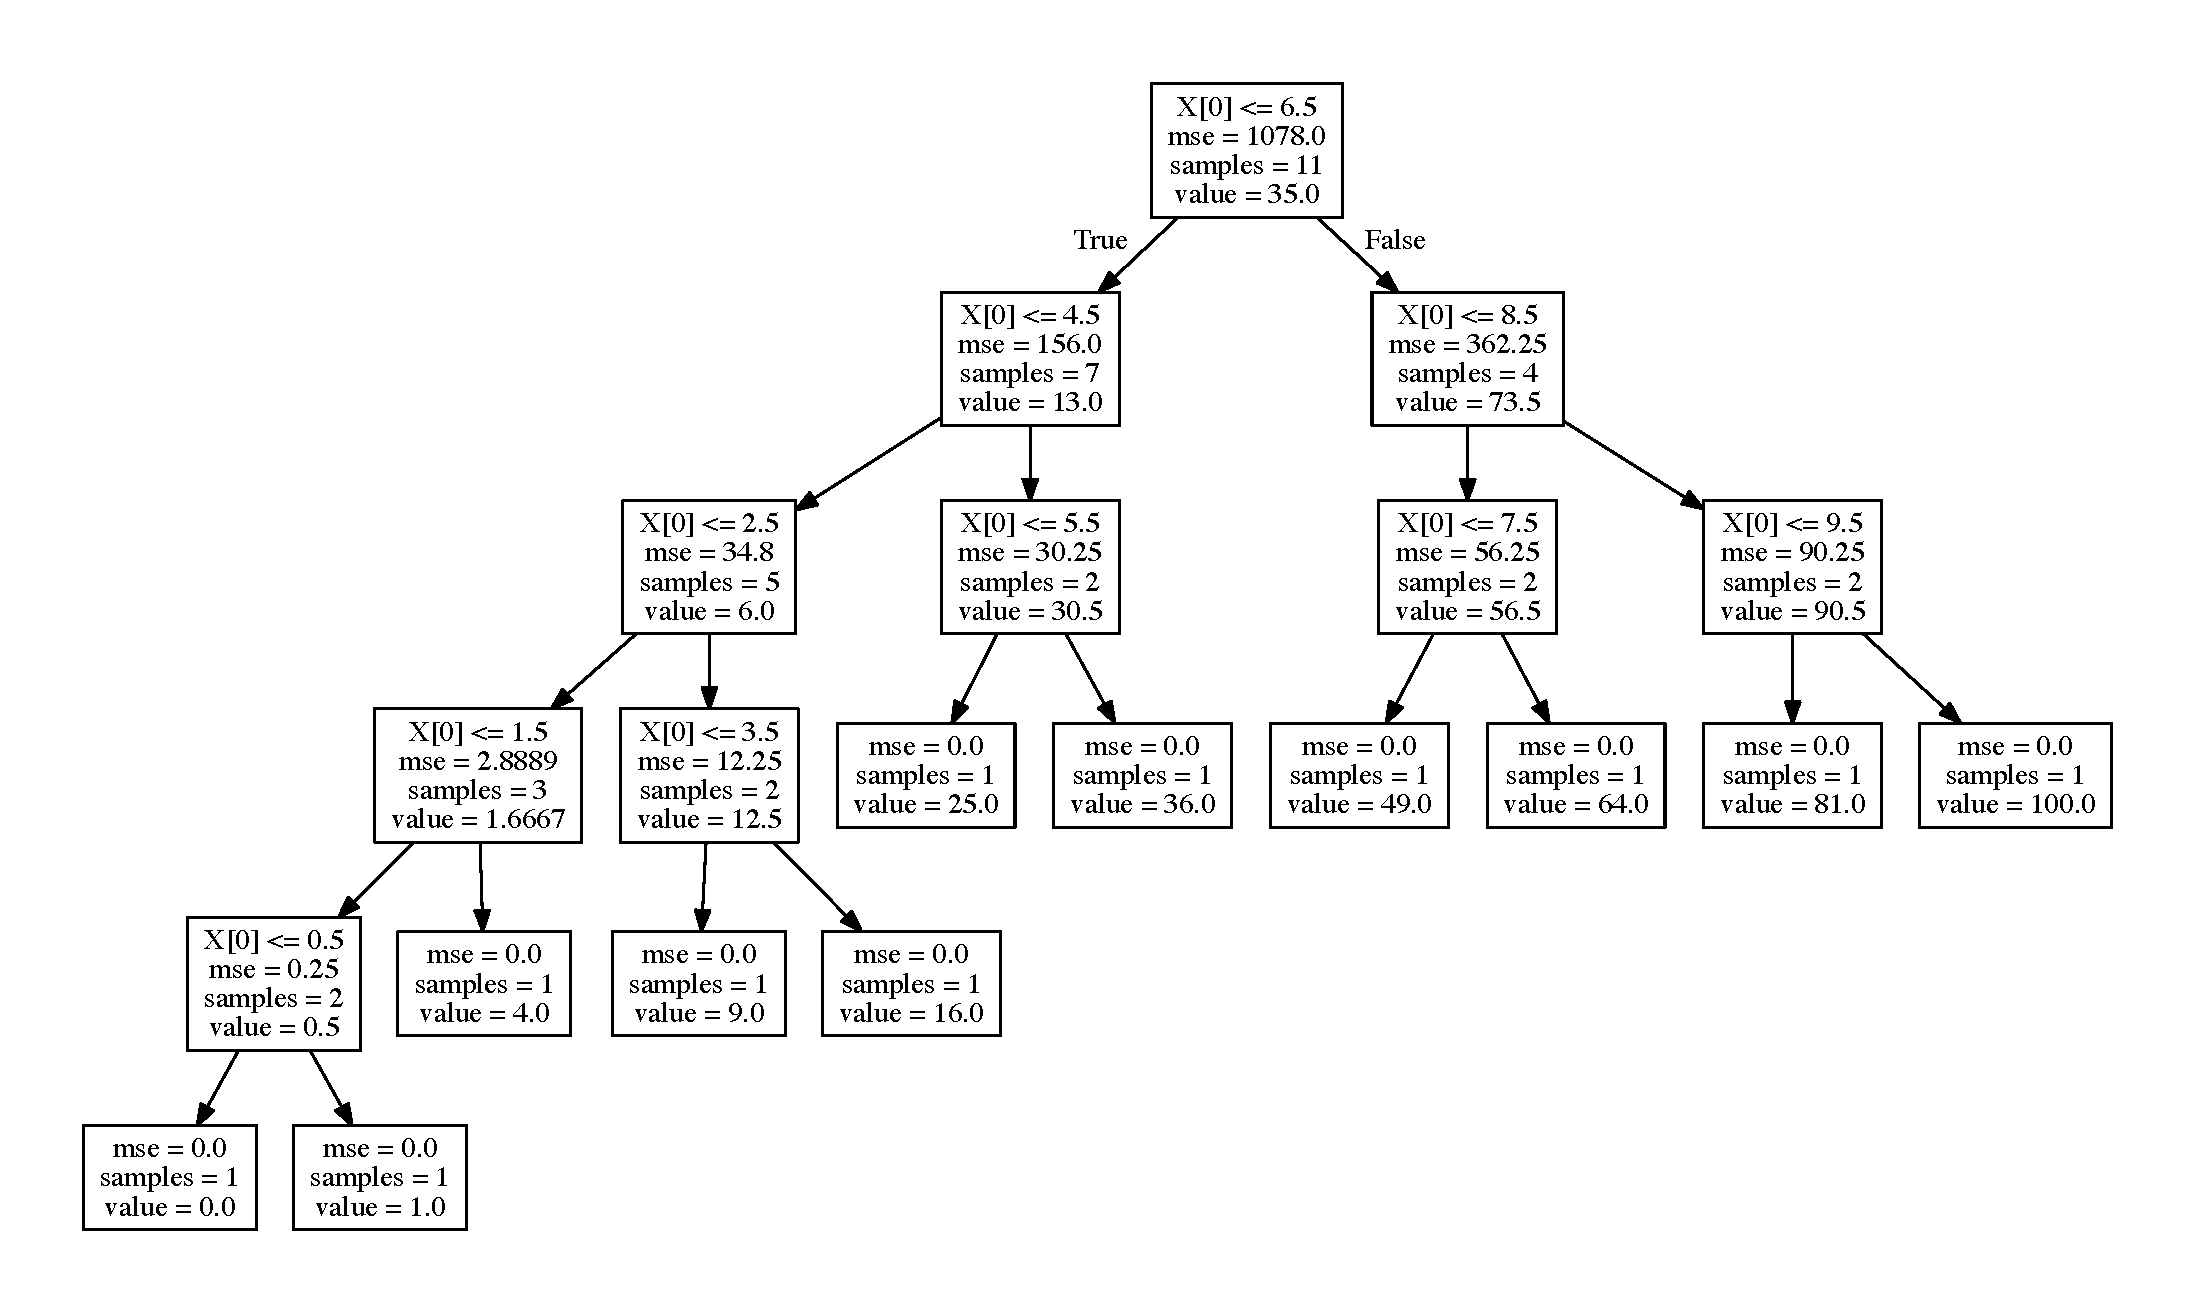
\includegraphics[width=\linewidth]{figures/reg_tree.pdf}
        \caption{Regression Decision Tree}
    \end{subfigure}
    \begin{subfigure}{0.49\textwidth}
        \centering
        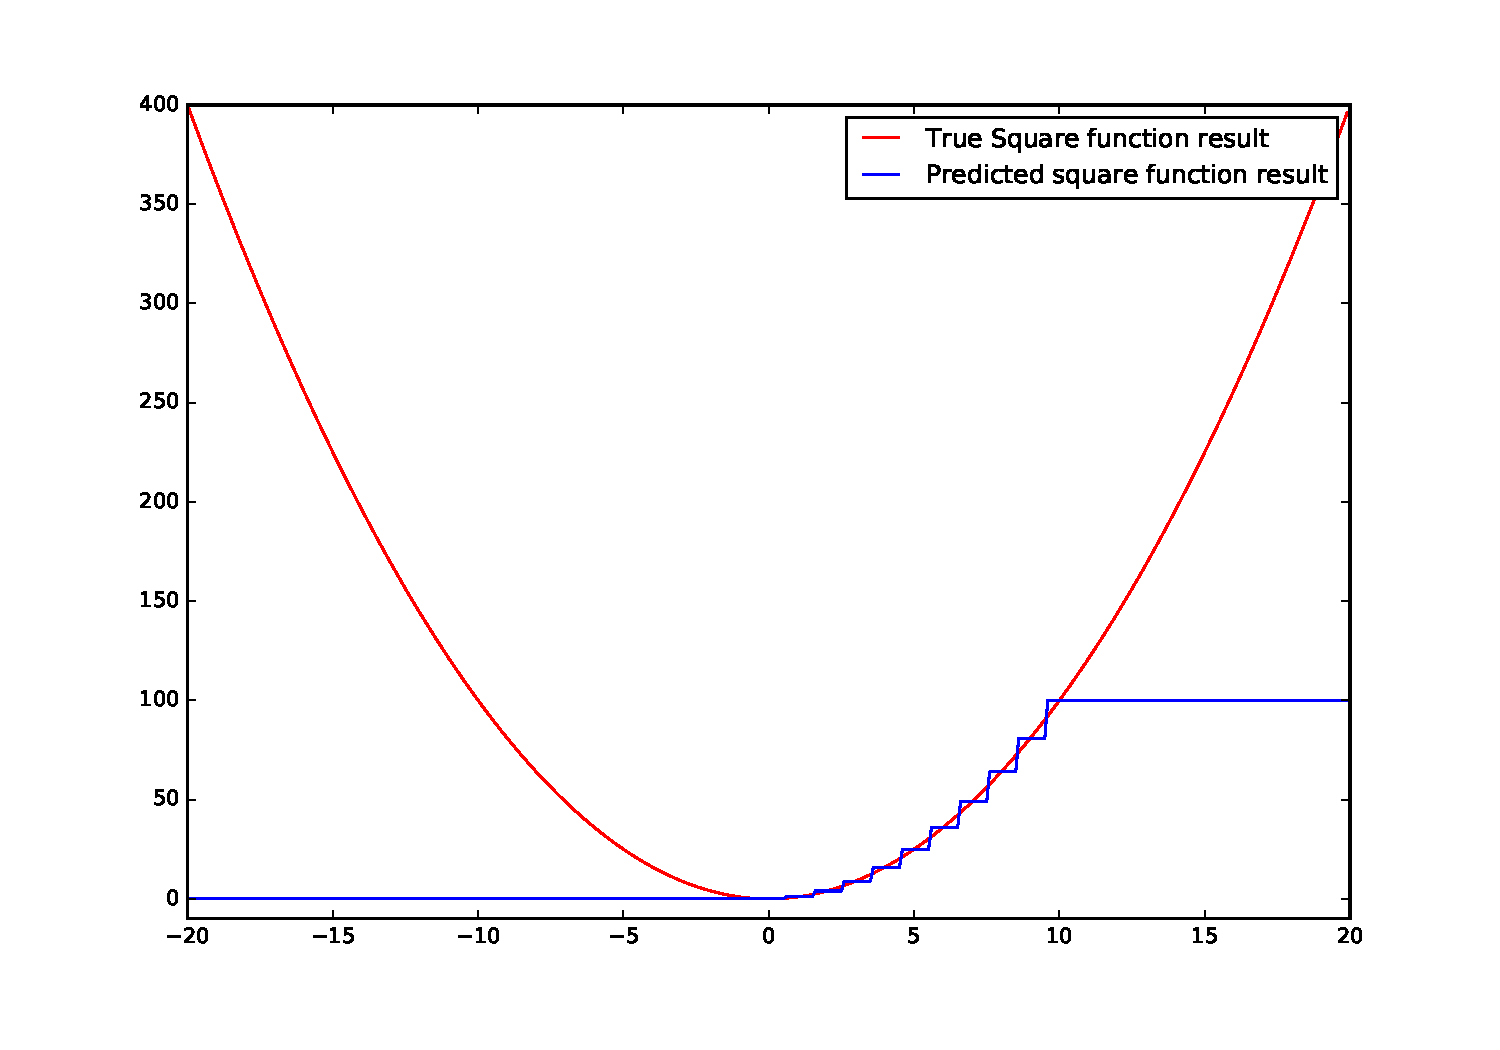
\includegraphics[width=\linewidth]{figures/reg_tree_plot.pdf}
        \caption{Regression Decision Test Results}
    \end{subfigure}
  \caption{A Decision Tree trained on a dataset of simple square functions, where the inputs were numbers from 0 to 10 and output is the square of each number. The tree shows a jagged approximation of the square function between 0 and 10, which indicates some level of learning. However, the tree shows very poor generalization outside the learning range. When tested on input that is below 0, the tree matches to the closest label in the decision boundary, which is "0". A similar decision is made for input that is greater than 10, where the trees matches all numbers greater than 10 to the label of 10 ("100").}
  \label{fig:decision_tree_regression_and_classification}
\end{figure}

From this small experiment, the need for a different approach to supervised learning is obvious. Such a technique would need to generalize the mapping not to categorical labels and their limited space, but to an unlimited range of numbers. This method would solve a more conventional mathematical problem of function approximation. Another way to think about the problem is curve fitting: given input and output sets, the curve of the approximated function should pass---or be proximal---the points given in the sets. The best fit for our function would be a curve that passes perfectly through all our data points. As the approximated curve moves further and further away from the given points, the distance between the points and the curve increases, which we can use as a measurement of error (Fig. \ref{fig:error_lines}). The sum of this error can be expressed as

\begin{figure}[!h]
  \centering
  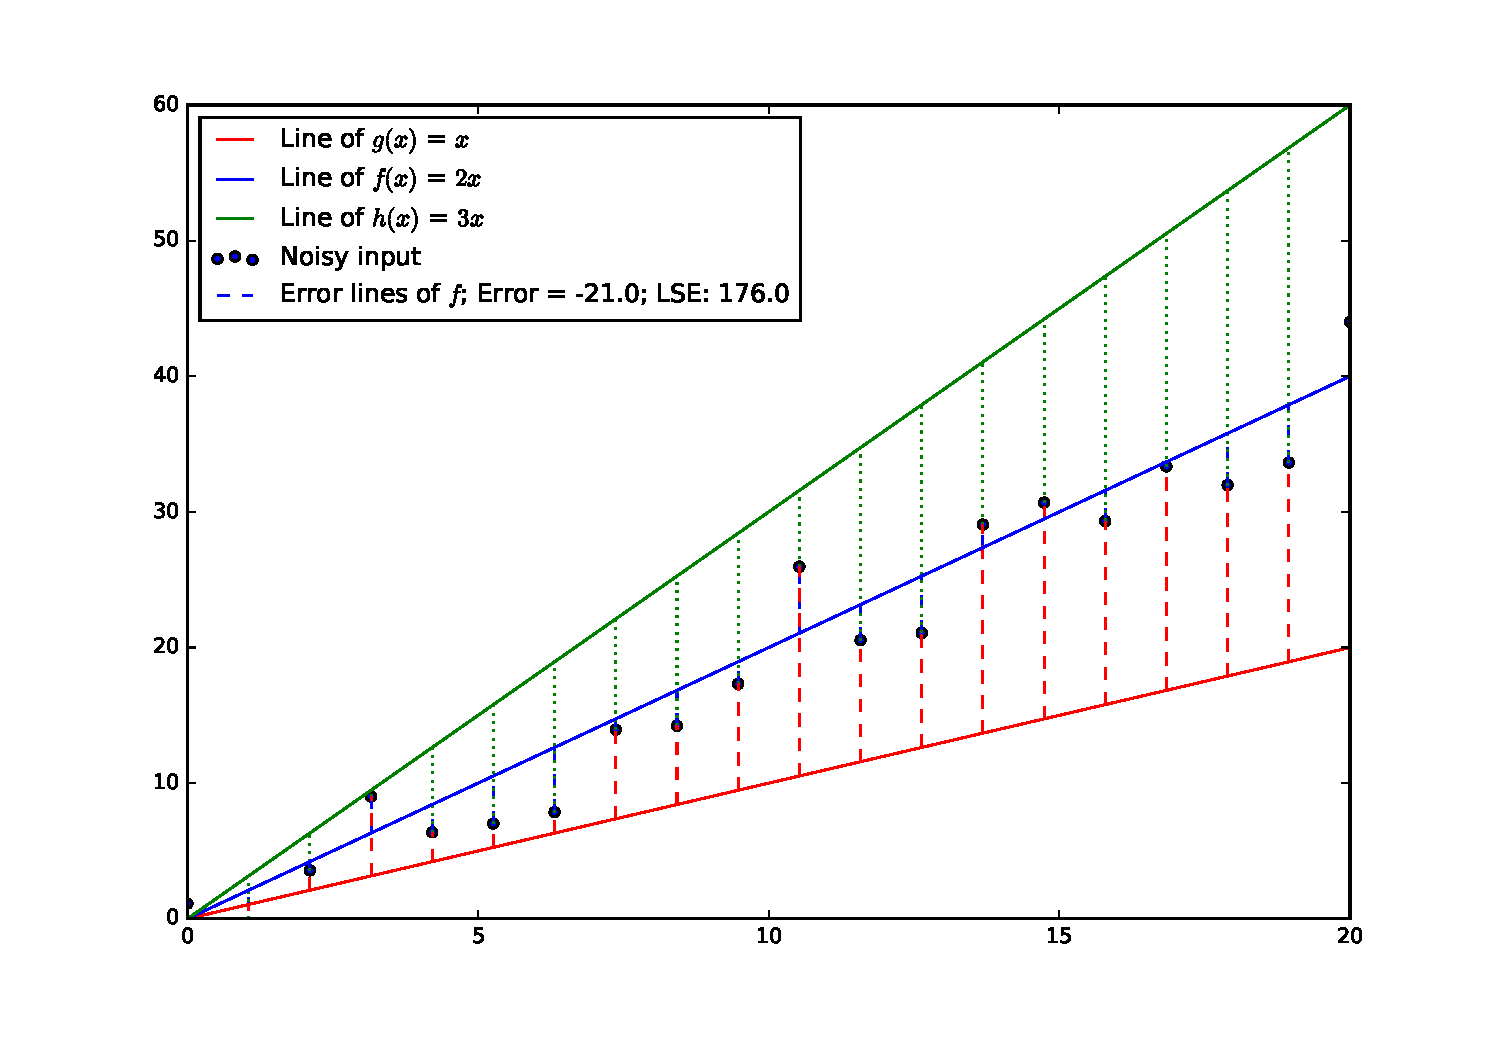
\includegraphics[width=0.7\linewidth]{figures/error_lines.pdf}
  \caption{Different lines of fit and their errors (dashed and dotted lines) with respect to the noisy input data. Because $g(x)$ and $h(x)$ have larger error lines than $f(x)$, $f(x)$ is the best fit for the data out of the three drawn lines. Note that for $f(x)$, the negative and positive errors cancel out, leading to a sum of error of $-21$. This is allayed by summing the square of the error instead, which results in an equation that can be minimized to $176$.}
  \label{fig:error_lines}
\end{figure}

\begin{align*}
  Error &= \sum_{i=1}^n (y_i-f(x_i)),
\end{align*}

where for the $i$th data point $y_i$ represents the actual $y$ value and $f(x_i)$ represents the approximation of the regression line at $x_i$. Minimizing this error term ensures that our resulting function is the closes line fit to our data points. However, notice that in our error function, positive and negative errors will cancel out, leading to the assumption that "two wrongs make a right". To avoid this, we can either take the absolute value of the error, or the square. For mathematical convenience, the squared error is preferred. This results in the method of Least Squared Error (LSE) as given by

\begin{align}
\label{eq:least_square}
LSE &= \sum_{i=0}^n (y_i-f(x_i))^2  = \sum_{i=0}^n (y_i- b_0 - b_1x_i)^2
\end{align}

From this equation it can be shown that 

\begin{align}
b_1 &= \frac{\sum_{i=1}^n y_ix_i - \frac{\sum_{i=1}^n y_i \sum_{i=1}^n x_i}{n}}{\sum_{i=1}^n x_i^2 - \frac{\Big(\sum_{i=1}^n x_i \Big)^2}{n}}
\end{align}

and 
$$ b_0 = \bar y - b_1 \bar x $$

where $\bar y$ and $\bar x$ are the respective means of all $y$ and $x$ values \cite{Finney1996}. This formula guarantees a line of best fit that minimizes squared errors for linear data points. For cases when the data points do not display a linear behavior, they can be transformed into a space where they become more linear, linear regression applied, and the regression functions transformed back into the original space (Fig \ref{fig:log_regression}).

\begin{figure}[!h]
  \centering
    \begin{subfigure}{0.32\textwidth}
        \centering
        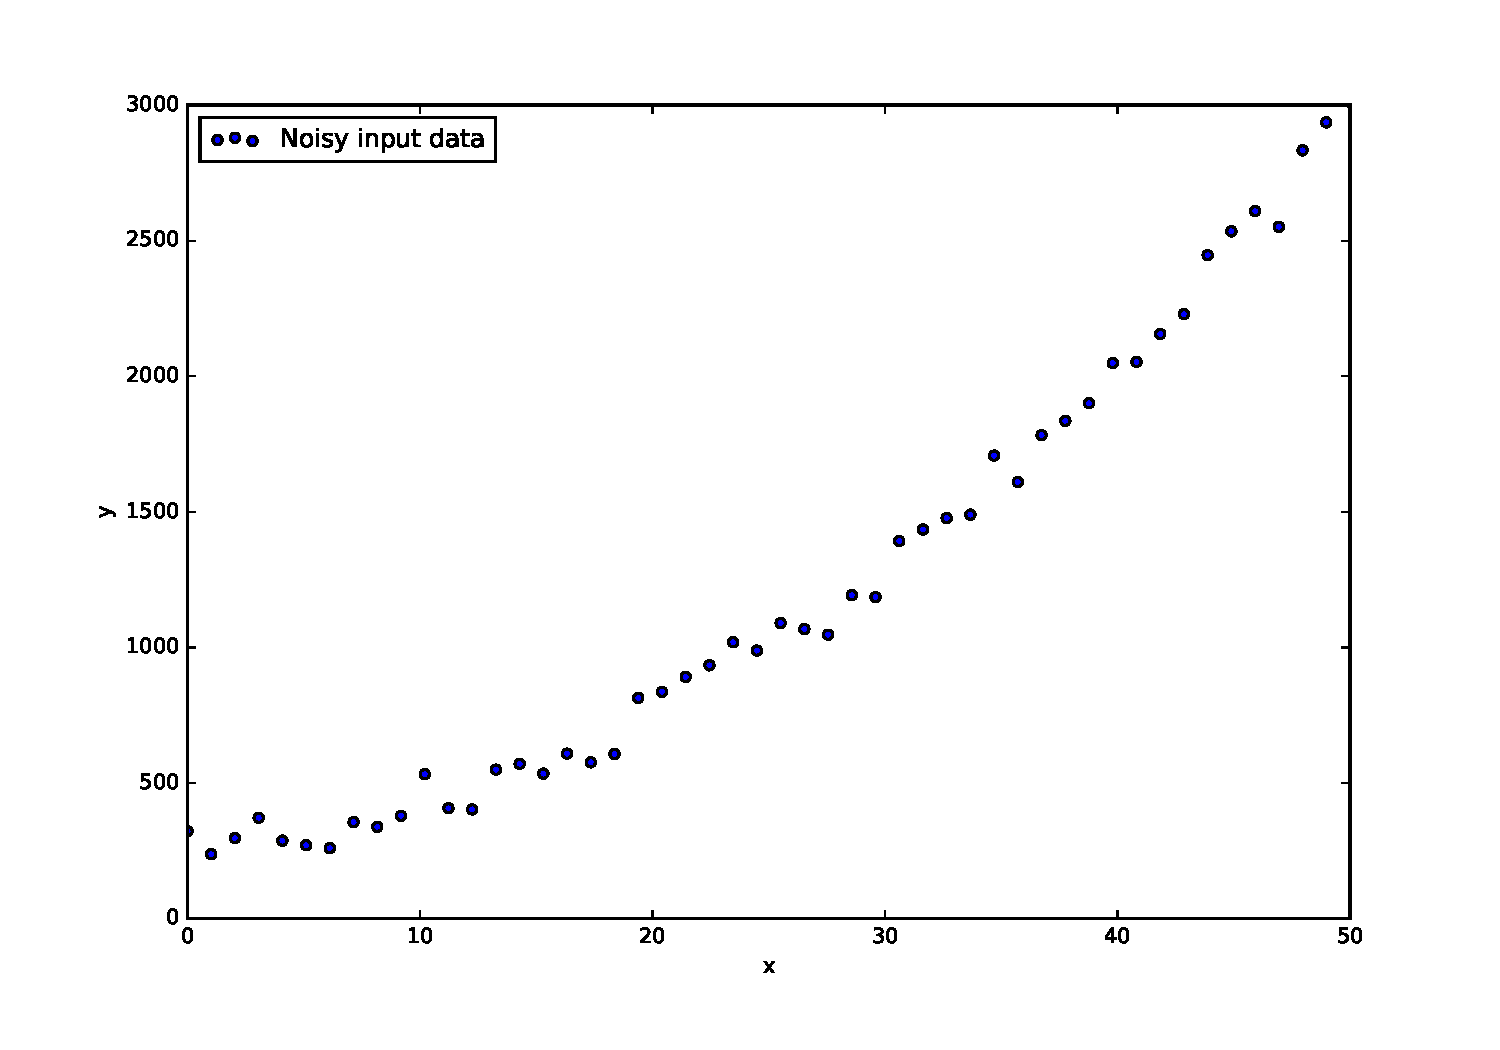
\includegraphics[width=\linewidth]{figures/regression_log_example_1.pdf}
    \end{subfigure}
  \begin{subfigure}{.32\textwidth}
        \centering
        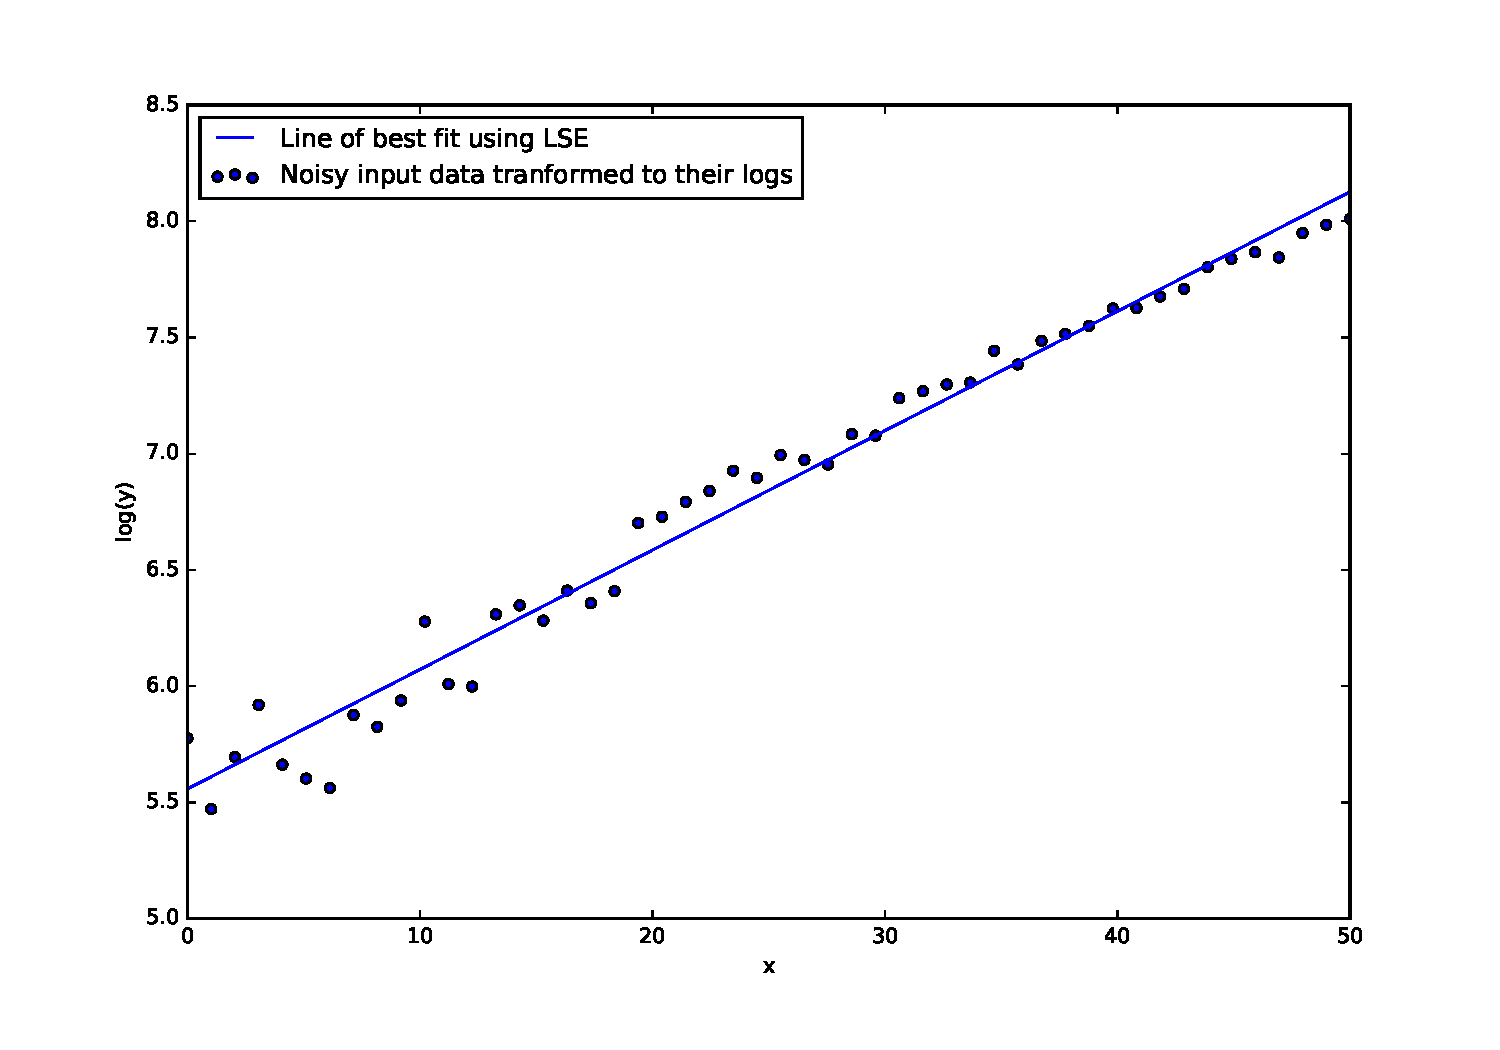
\includegraphics[width=\linewidth]{figures/regression_log_example_2.pdf}
    \end{subfigure}
    \begin{subfigure}{0.32\textwidth}
        \centering
        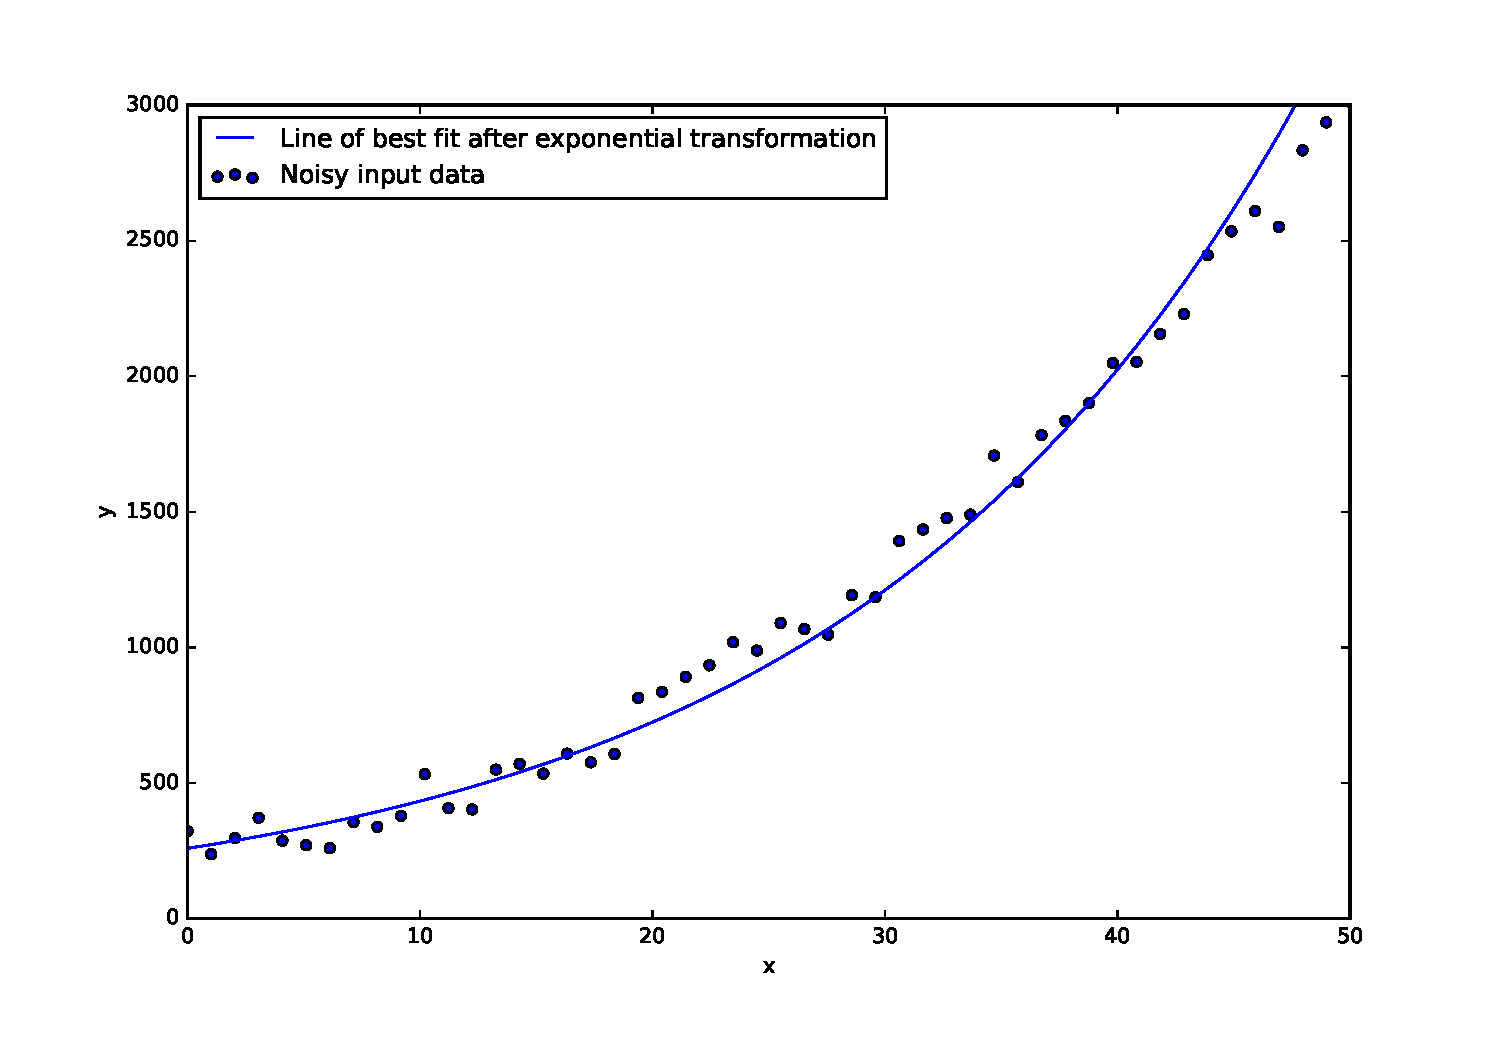
\includegraphics[width=\linewidth]{figures/regression_log_example_3.pdf}
    \end{subfigure}
  \caption{Finding line of least squared error for data with an exponential trend. First, the data points (Left) are transformed to their logs (Center). Then a line of best fit is found through linear regression (Center). The line is then transformed back to the original space by applying the exponential function (Right).}
  \label{fig:log_regression}
\end{figure}

Using this regression model for out previous example in Figure \ref{fig:decision_tree_regression_and_classification}, we are able to attain more realistic learning through a model that extrapolates more correctly to unseen numeric data (Fig. \ref{fig:regression_on_square_function})

\begin{figure}[!h]
  \centering
    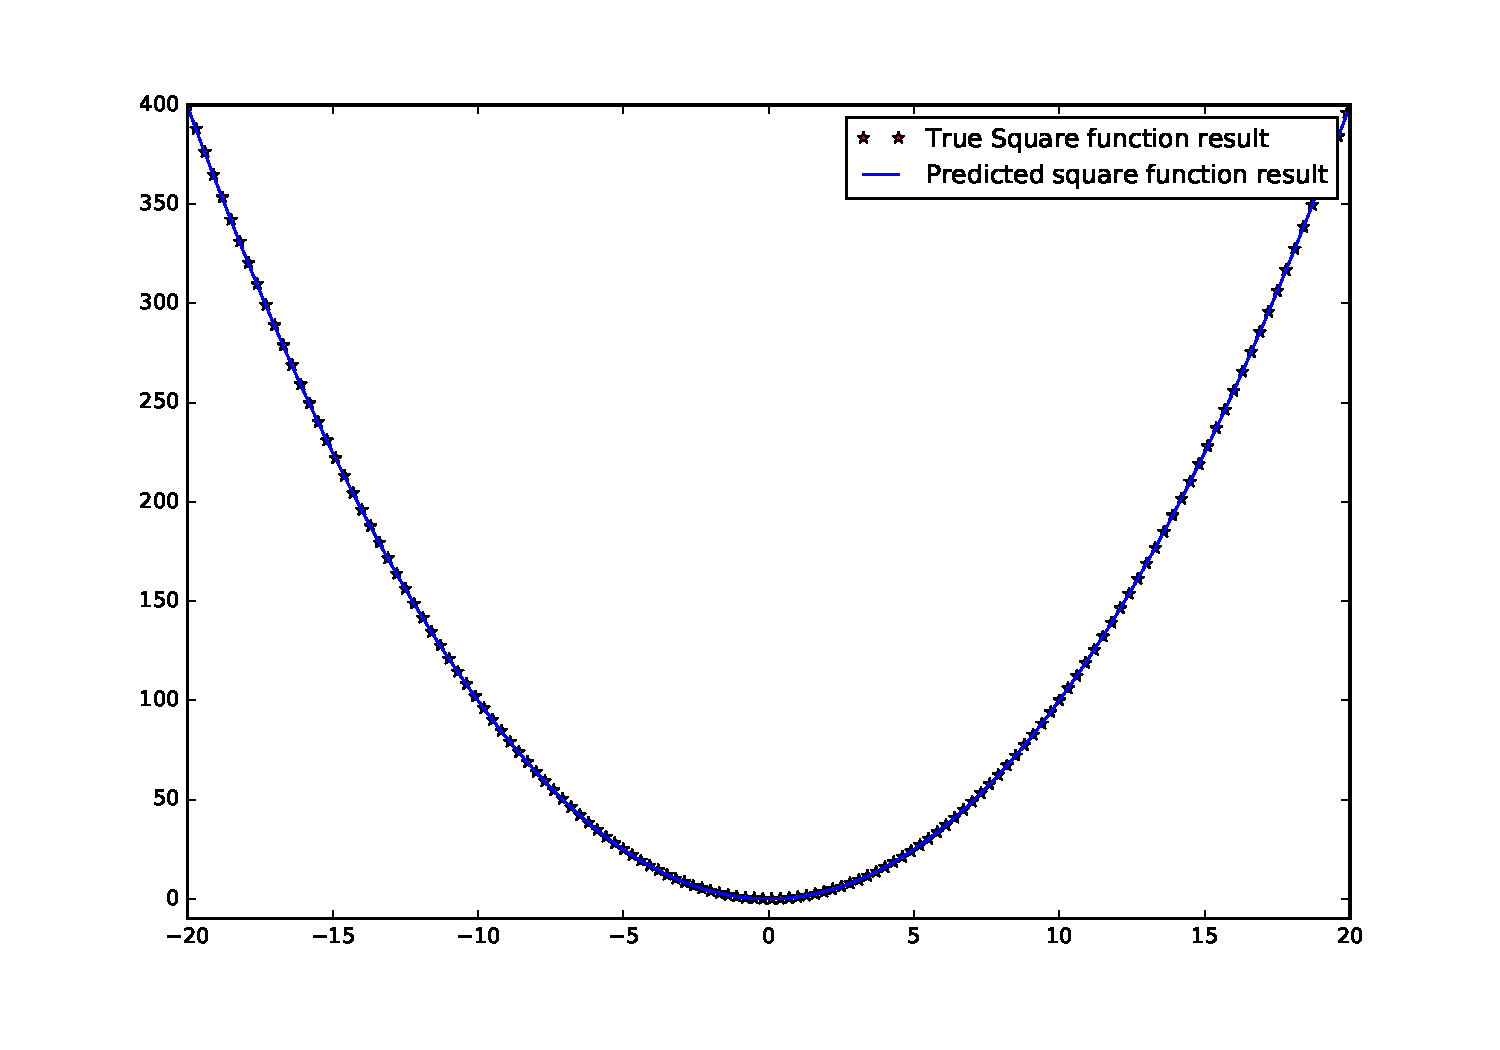
\includegraphics[width=0.7\linewidth]{figures/reg_ridge_plot.pdf}
  \caption{Using a non-linear regression model for the same data set used on in Figure \ref{fig:decision_tree_regression_and_classification}, we are able to build a model that correctly extrapolates to unseen numeric data. Since this is one of the requirements for problems with outputs being continuous numbers, thsi model is highly valuable for prediction in such output spaces.}
  \label{fig:regression_on_square_function}
\end{figure}
%We might be able to include support vector machines.
\subsection{Unsupervised Learning}
While supervised learning aims to entangle patterns by examining data that has been labeled by humans, unsupervised learning attempts to do the same with unlabeled data. This requires algorithms that can examine unstructured information and find commonalities and dissimilarities between data points. Humans are exceptional at unsupervised learning, performing tasks of separation and discrimination from a young age. For example, children "can discriminate faces and voices by sex, habituate to faces of both sexes, and make inter-modal associations between faces and voices" \cite{martin2010patterns}. These skills to separate items based on patterns are also evident in our everyday lives: we separate tasks into work, pleasure, or home-related categories; cars into new, old, attractive, or boring; restaurants into lower-end (e.g. McDonalds) or high-end (e.g. Red Lobster); people into races. In most if not all of the previous cases, we are not \textit{told} what items belong to what categories, and in fact we are not told what the categories are. Rather, we assume that there are some categories, and we attempt to distribute items into the categories that make the most sense to us. This human ability to discern patterns from unstructured data is similar to how unsupervised learning works.

With most unsupervised learning algorithms, the number of categories is known or guessed, and it is the job of the algorithm to separate the data into that many categories in the best possible way. A plethora of unsupervised learning algorithms exist, most of which are extensions on more basic and fundamental ones. Some of the fundamental algorithms include K-means clustering, fuzzy clustering, single linkage clustering, self organized maps, and vector quantization. For the purposes of this work, we only cover the simple K-means algorithm, an extension of which we use in the experimental section of this paper.

\subsubsection{K-means Clustering}
K-means clustering is a powerful tool used in various fields mainly for cluster analysis. It operates on basic principles of finding subsets of data that share the most commonality between one another. This algorithm requires the data to be in continuous numerical form, and uses one of several measures of distance to attribute closeness. The most widely used measure of distance is the Euclidean distance 
$$
D(x, y) = \sqrt{(x_1 - y_1)^2 + (x_2 - y_2)^2 + \dots + (x_n - y_n)^2}.
$$
K-means works by finding $k$ centers of clusters, where $k$ is the number of hypothesized clusters given by the user. This goal is achieved by first choosing $k$ random points from all the points in the given dataset. All the remaining points are then matched with the closest center, and each matched set of points is declared as a cluster. For centers $c_1, c_2, \dots, c_n$ and point $x$, $x$ belongs to the cluster whose center is the closest to $x$ 
$$
Cluster(x) = \arg \min_{c} \Big( D(c_1, x), D(c_2, x), \dots, D(c_k, x) \Big).
$$
Once all the points have been assigned to a cluster, an approximate center point of each cluster is calculated as the mean of all the points in that cluster
$$
\hat c_i = mean(x_{i,1}, x_{i,2}, \dots, x_{i,l})
$$
where $x_{i,j}$ is the $j^{th}$ point in the $i^{th}$ cluster.
A new center for the cluster, $c_i$, is then chosen, with the new center being the closest to the approximate center point
$$
c_i = \arg \min_{x} \Big( D(\hat c_i, x_{i, 1}), D(\hat c_i, x_{i, 2}), \dots, D(\hat c_i, x_{i, 2}) \Big ) .
$$
This will result in a change of points-to-cluster-center distances, and will therefore change the clusters that some points belong to, which will change the cluster centers, resulting in a cycle of improvement that has been proven to converge with the repetition of the center assignment steps (Fig. \ref{fig:k-means}). While the K-means algorithm is useful in its own right, extensions have made it more powerful. An example of such an extension is the Gaussian Mixture model, which is a more generalized form of the K-means that assumes there are $k$ uniform distributions with unknown parameters. This generalization allows the model to group clusters using several covariance shapes, meaning the distance relationships are much more diverse and flexible (Fig. \ref{fig:gaussian_mixture}) .

\begin{figure}[!h]
  \centering
  \begin{subfigure}{.3\textwidth}
    \centering
    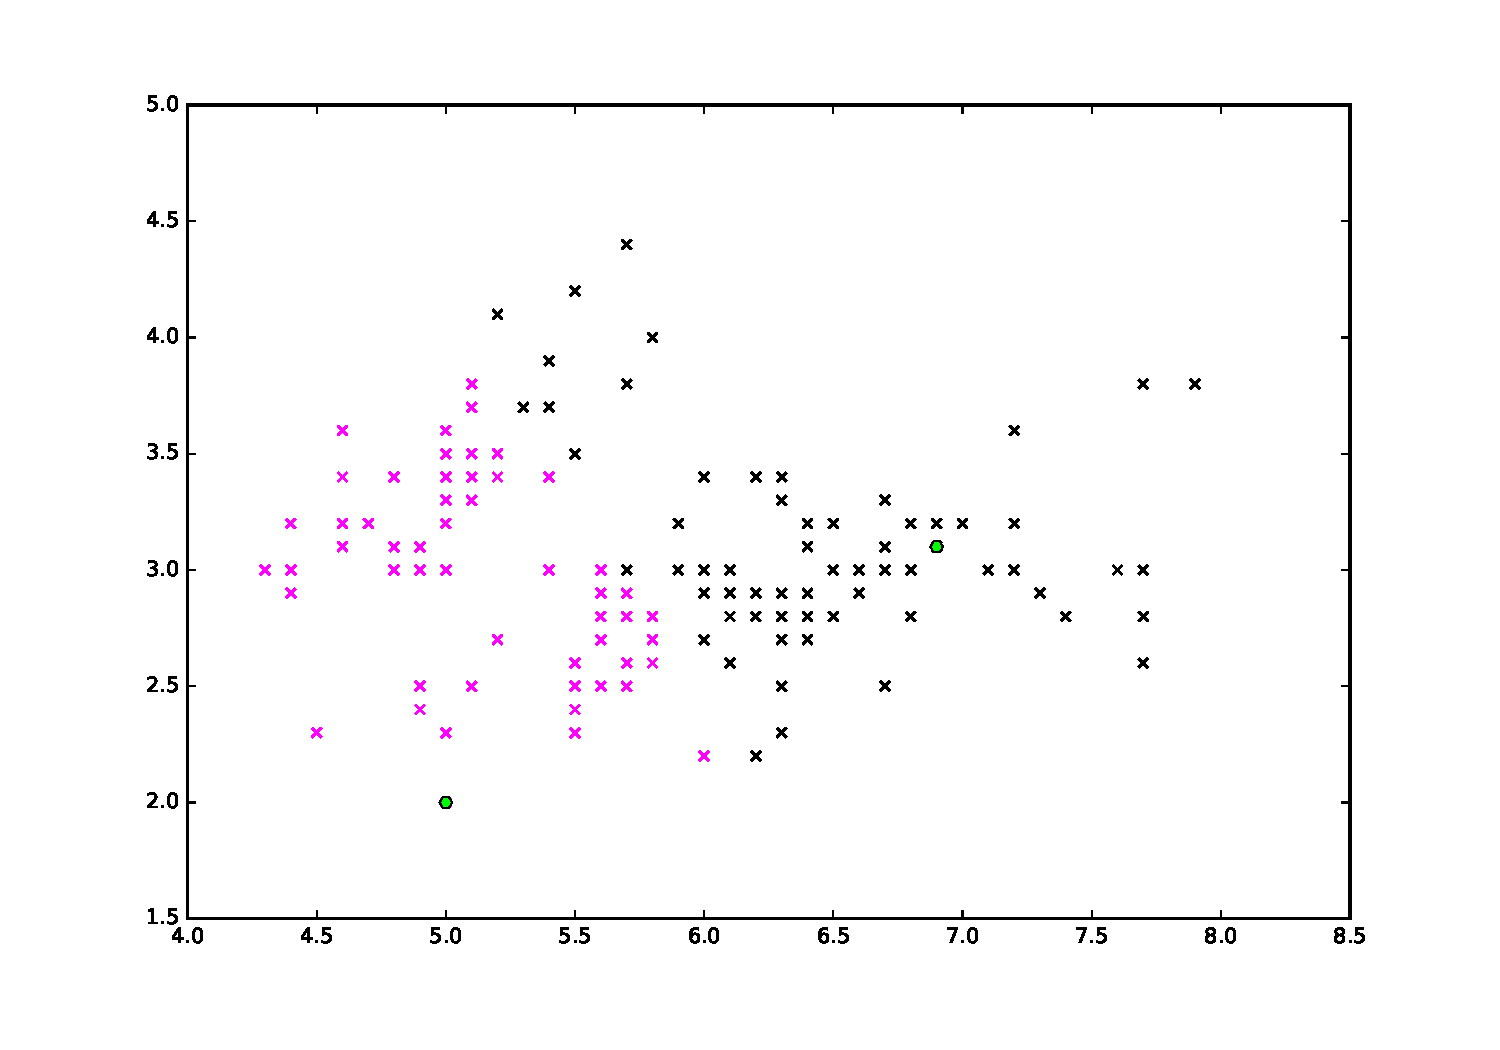
\includegraphics[width=\linewidth]{figures/k-means_first_1_iteration.pdf}
    \caption{Iteration 1}
  \end{subfigure} %
  \begin{subfigure}{0.3\textwidth}
    \centering
    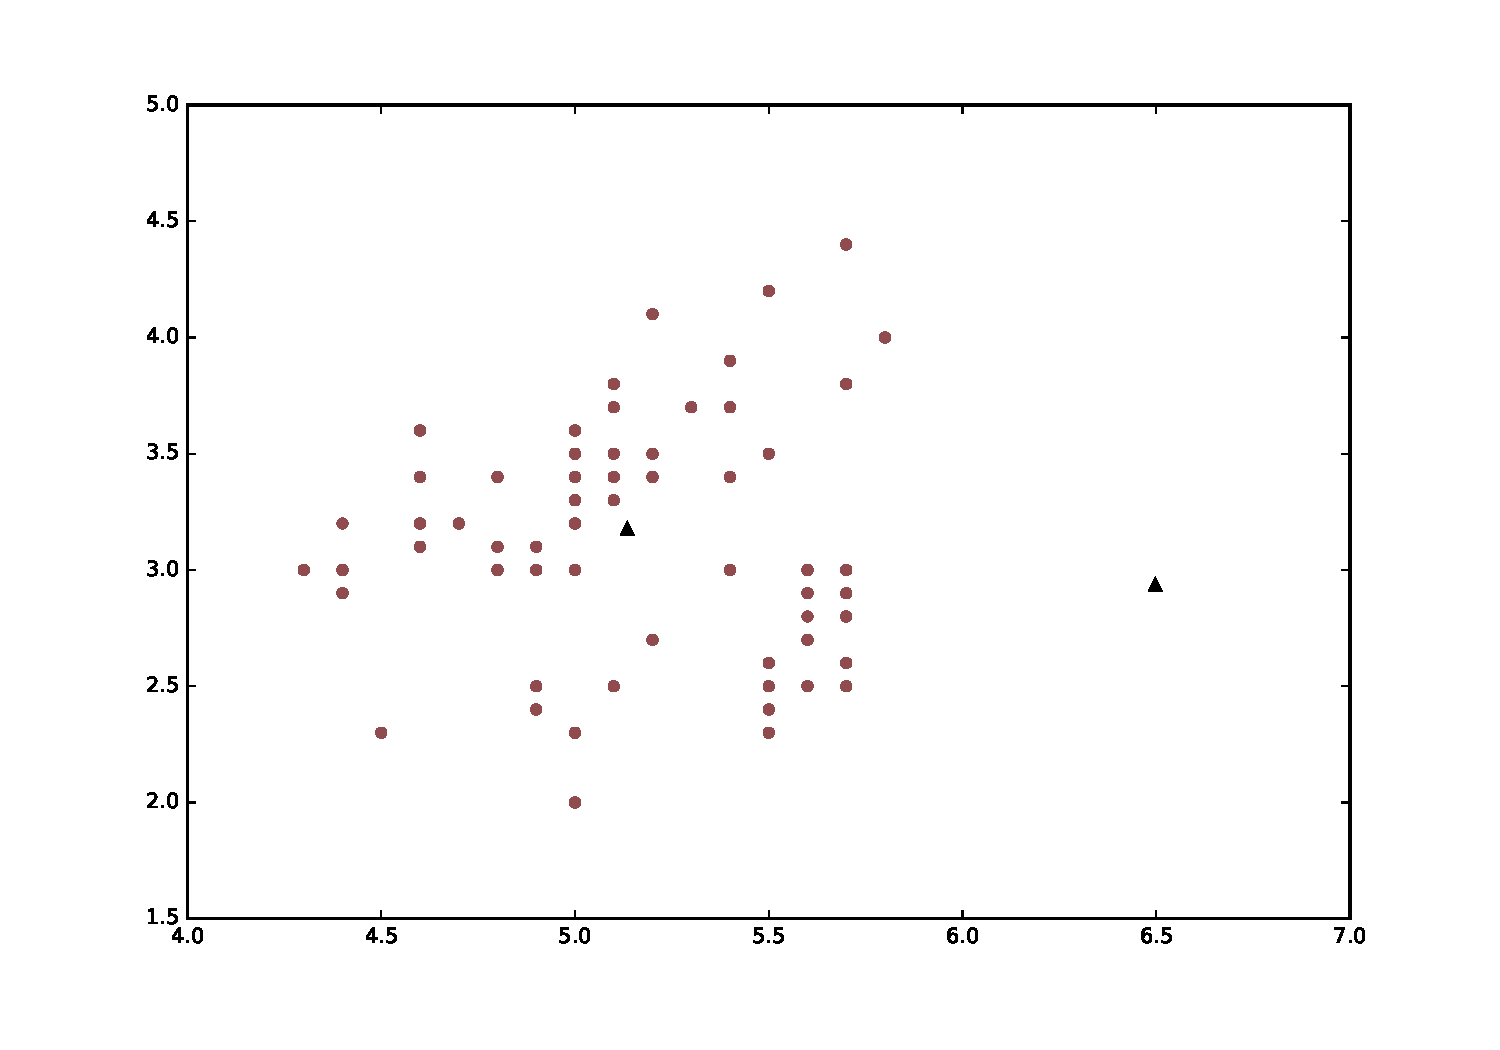
\includegraphics[width=\linewidth]{figures/k-means_first_2_iteration.pdf}
    \caption{Iteration 2}
  \end{subfigure}
	\begin{subfigure}{0.3\textwidth}
		\centering
		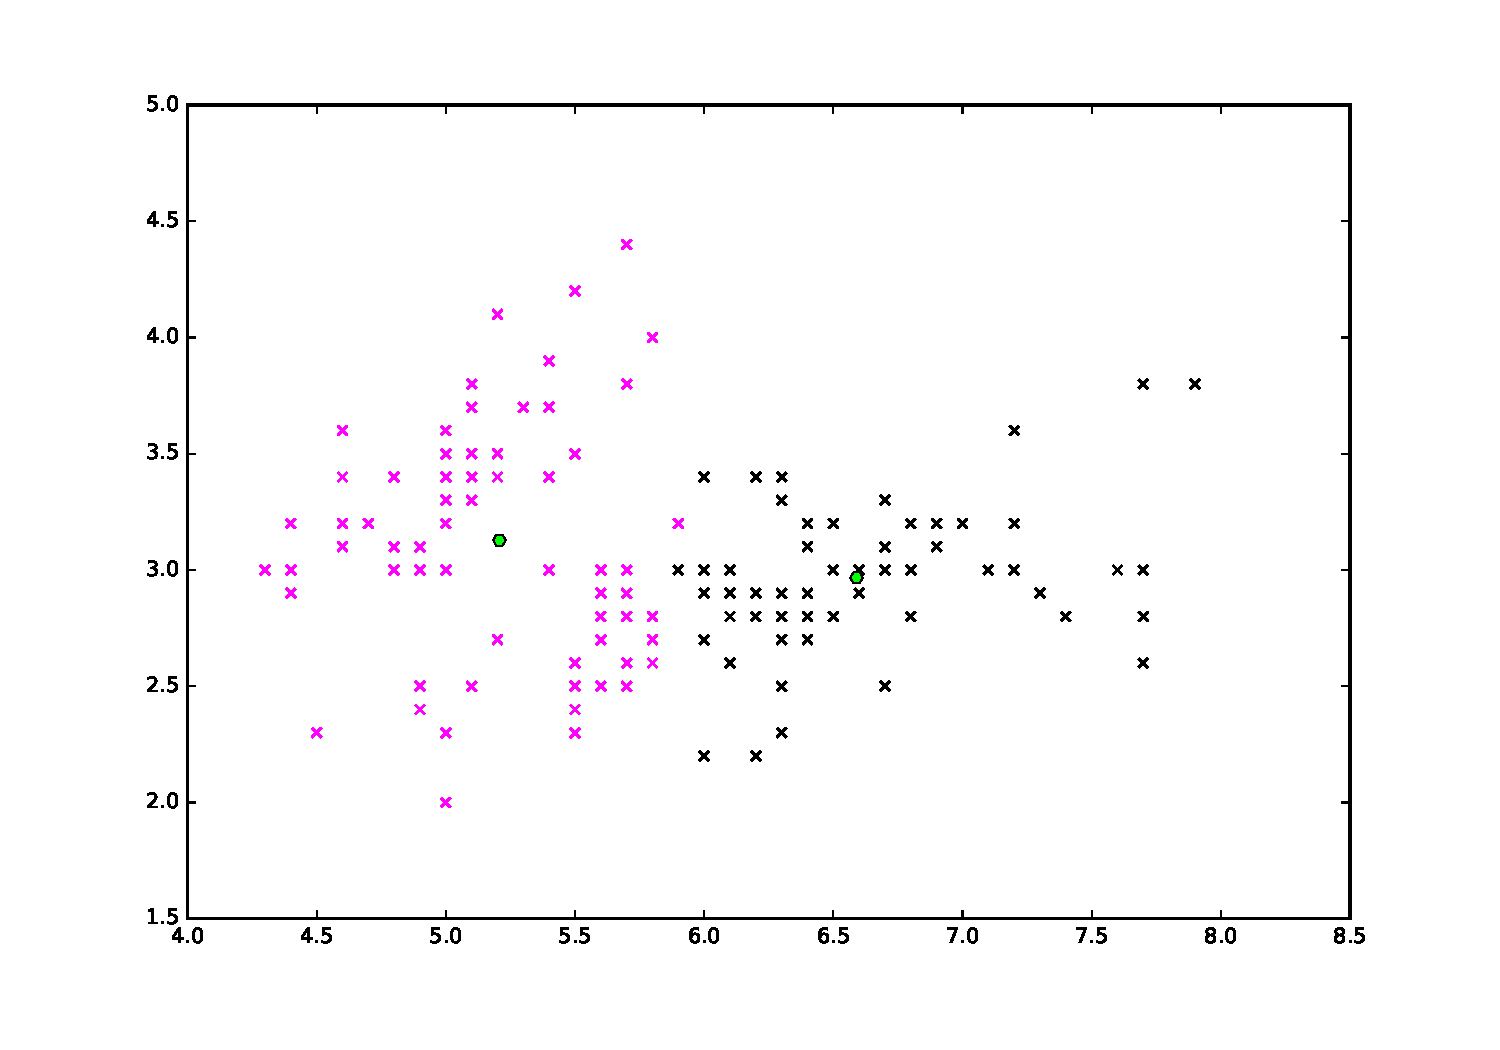
\includegraphics[width=\linewidth]{figures/k-means_first_5_iteration.pdf}
		\caption{Iteration 5}
	\end{subfigure}
  \caption{A sample iteration of simple k-means clustering on the generally available Iris dataset. The clusters are shown in different colors, while the centers are the green circles. In the first iteration, the centers are randomized along the dataset. As the algorithm iterates, it finds more representatives cluster centers which split the dataset more evenly, until it converges in step 5.}
  \label{fig:k-means}
\end{figure}

\begin{figure}[!h]
  \centering
  \begin{subfigure}{.4\textwidth}
    \centering
    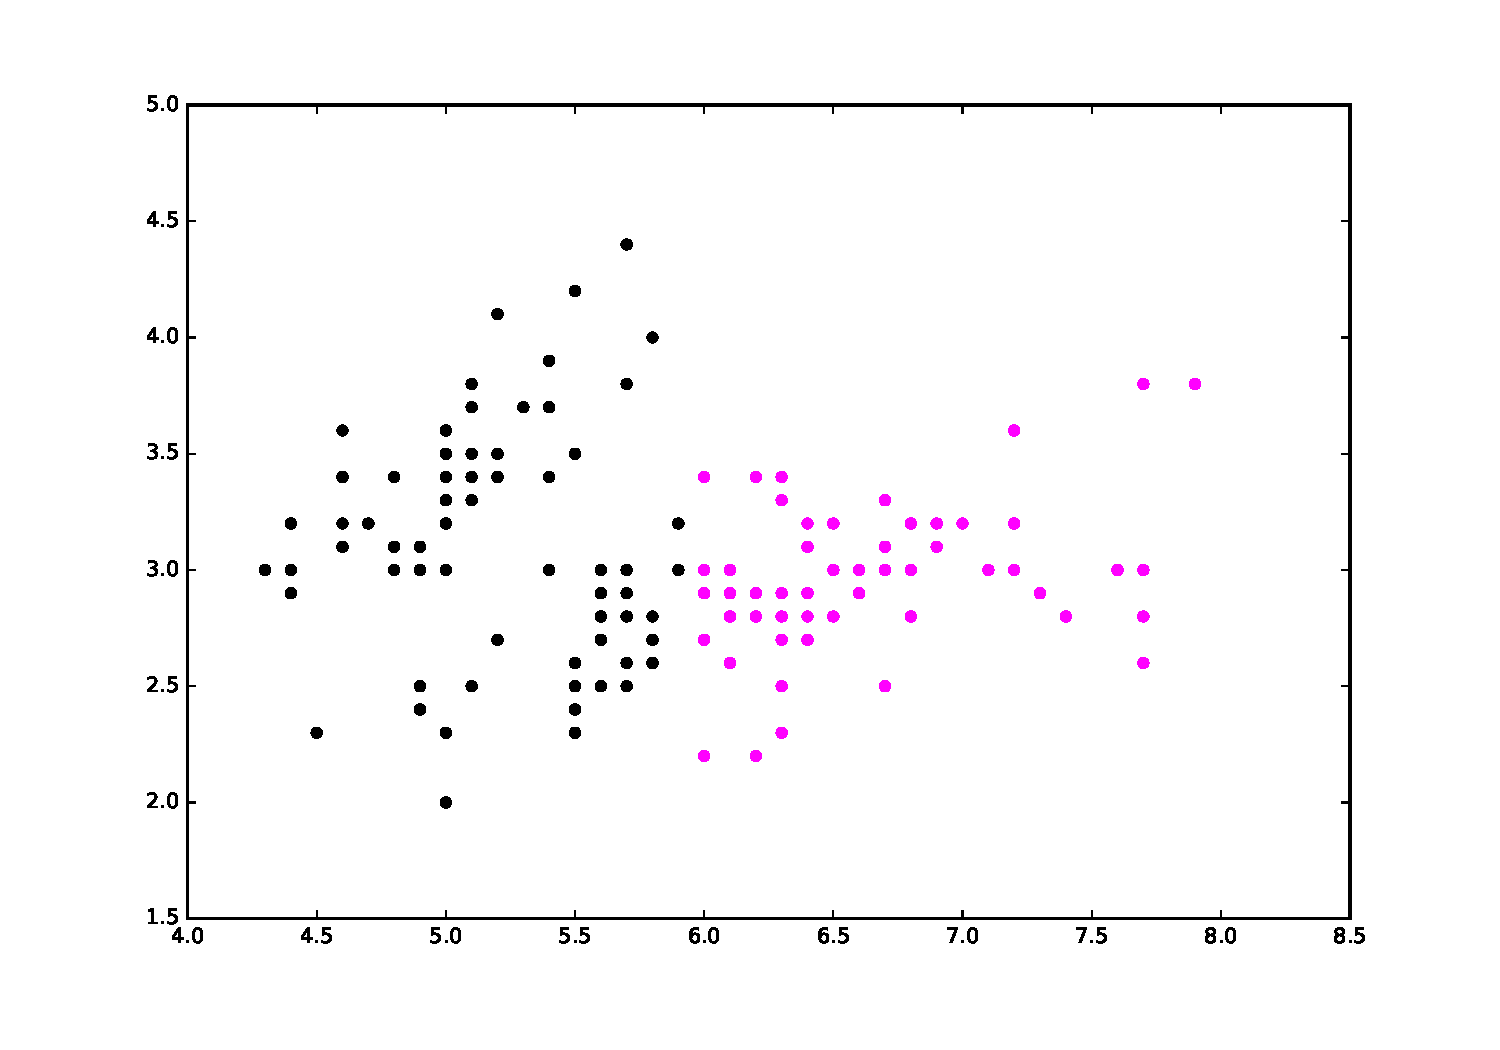
\includegraphics[width=\linewidth]{figures/simple_k_means_iris.pdf}
    \caption{Simple k-means}
  \end{subfigure} %
  \begin{subfigure}{0.4\textwidth}
    \centering
    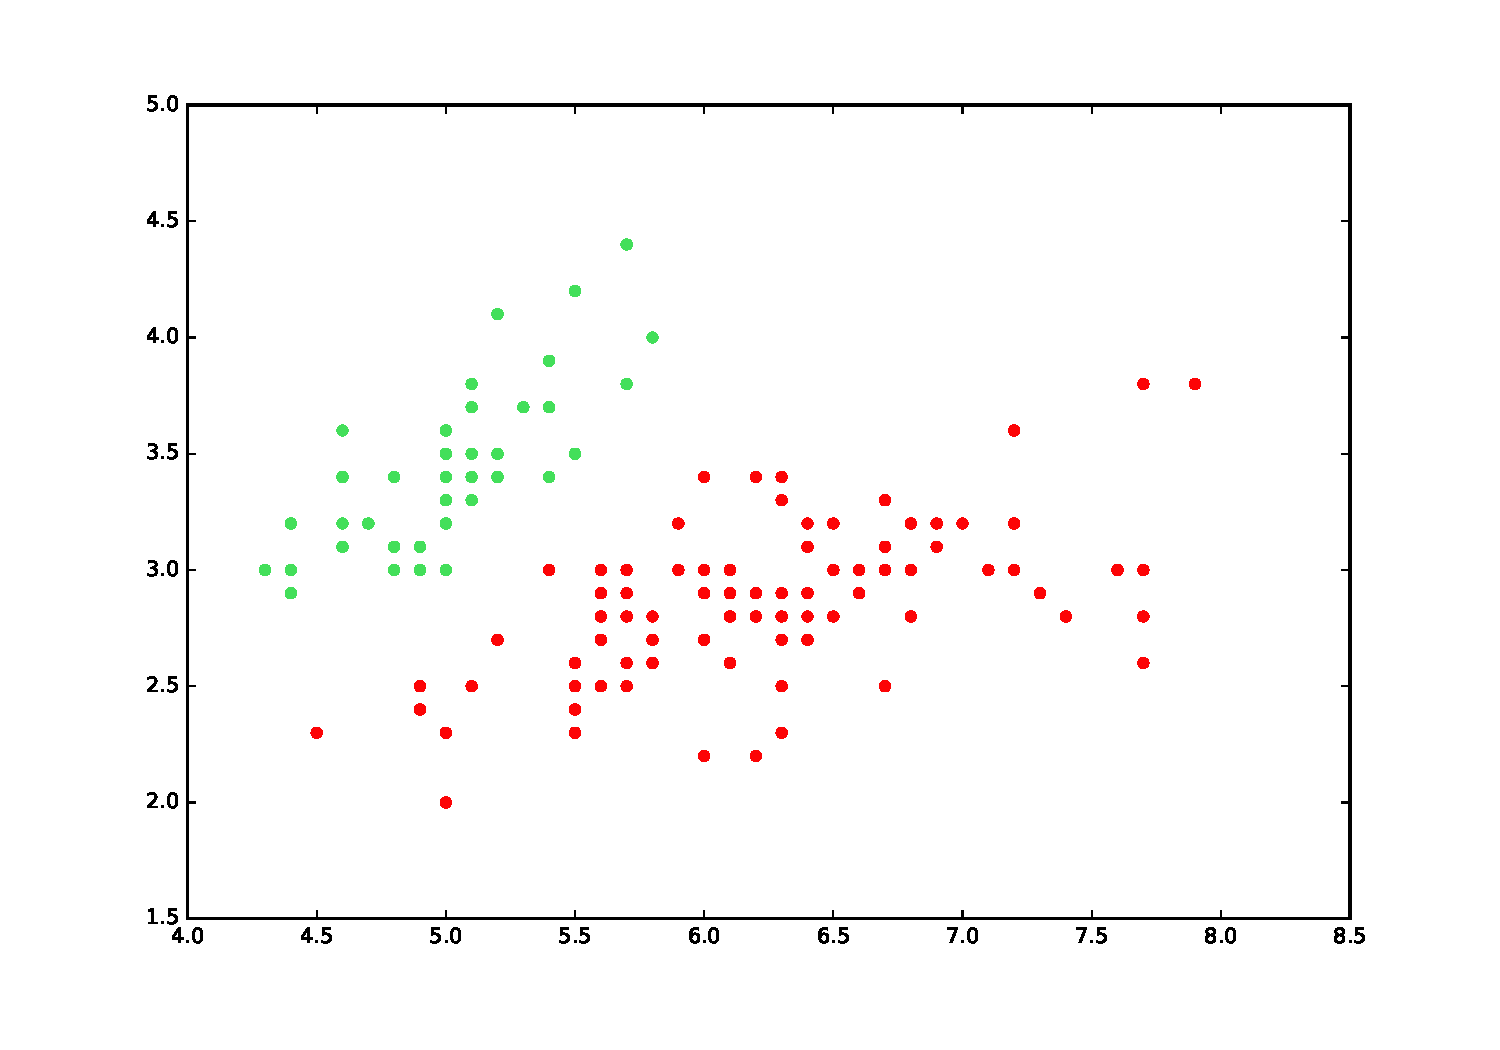
\includegraphics[width=\linewidth]{figures/gaussian_mixture_iris.pdf}
    \caption{Gaussian Mixture}
  \end{subfigure}
  \caption{While the standard k-means algorithm splits the dataset in the most even way, that does not necessarily result in a meaningful or accurate separation of clusters. The Gaussian Mixture algorithm takes advantage of more assumptions such as assuming that the clusters are produced from $k$ different normal (or Gaussian) distributions, and attributes points to clusters that make these distributions the most likely. This usually results in a more meaningful approach and result, as many natural phenomena are indeed a product of the Gaussian distribution.}
  \label{fig:gaussian_mixture}
\end{figure}
% \subsection{Reinforcement Learning}
\section{Sugihara Causality}
The concepts of abstract correspondence, correlation and interpreting causation has been discussed in philosophical literature at least as early as Berkley's and Locke's arguments on human perception \cite{Locke1841} \cite{Berkeley1874}. Until now, the debate focused on what constitutes a causative effect and how such an effect might be discerned. From philosophy, the debate has moved to empirical science, where different models of causality have been proposed, none of which has been declared the true standard. Causality is often mistaken for correlation because the relationship between the two is not always clear. For example, falling down the stairs could be correlated with breaking a limb, but is falling down the stairs caused by breaking a limb, or is breaking a limb caused by falling down the stairs? One might argue that a person wouldn't break a limb without falling down the stairs, but what if a limb was stressed enough that it broke while a person was normally walking down the stairs, causing the person to lose control of their leg and therefor fall? In this sense, causality is a murky subject that is often considered to be highly subjective and at times nondetachable from the context of the situation. With that being said, there have been many attempts to address the concept of causality in mathematics in the form of the causality of continuous signals on one another. For example, if one could attain the stock prices for hot dogs and hot dogs buns, one would be able to hypothetically see a correlation between the sales of hot dogs and hot dog buns. It is also clear that one can describe a logical causation between the two stock prices, since the products are complementary to one another: if the price for one goes down, the price for the other goes down as well. For the case when substantial fluctuations happen in the stock price for both products, how would one determine which product caused the change in the price of the other? Surely the price drop was caused by \textit{something}, so which of the products caused the other? This is where causality models come into play---this is an example of the use of causality models in the field of Economy.

A particular causality model, Granger Causality (GC), has been widely used in application in the econometric fields \cite{Granger1969}, and has been the de facto model when causality is concerned. The way Granger Causality works is beyond the scope of this paper, but suffice it to say that Granger Causality behaves best in linear, stochastic systems. However, this causality model carries its own limitations, as, even with extensions to non-linear systems, it has generally not been seen capable of inferring causality in deterministic systems where feedback loops and nonlinearity are a defining feature. New models of causality have been introduced to attempt to go beyond these limitations. Dynamic Bayesian Networks and, more recently, the Convergent Cross Mapping (CCM) are some such models. The CCM model, also called Sugihara Causality model, relies on the convergence of distance of nearest neighbors in the shadow manifold of pairs of variables \cite{Sugihara2012}. To understand what all this means, we must first discuss manifolds (also called attractors).

\subsection{Manifolds}
Given three time series, a manifold of those three series is a new, three-dimensional representation of the state of the three variables at each time point. If the time series are somehow related to a specific concept, then this concept is called a \textit{system}, and the manifold then represents the state progression of the system. To illustrate this, a common example is used, namely the Lorenz Attractor. The Lorenz system is made up of three time series that are governed by the following differential equations

\begin{align}
\frac{\partial x}{\partial t} &= \sigma(y-x) \\
\frac{\partial y}{\partial t} &= x(\rho-z) - y \\
\frac{\partial z}{\partial t} &= xy- \beta z
\end{align}

where $\sigma$, $\rho$, and $\beta$ are constants \cite{lorenz1963deterministic}. With an initial condition and some time steps, we can produce three time series like in figure \ref{fig:lorenz_time_series}. Given these three time series, a manifold $M$ can be constructed by creating a new time series from the combination of these three series such that each time point $t$ in the manifold, $M_t$, is described as 

$$M_t = (x_t, y_t, z_t).$$

Of course, since this manifold has information about all the three previous time series, it is more highly dimensional than the time series themselves. In this case, since the manifold is of three time series, it is three dimensional (Fig. \ref{fig:lorenz_attractor}). Furthermore, since the manifold completely encapsulates the information about the system, the time series $x$, $y$, and $z$ can be generated if one has access only to the manifold of the system.

\begin{figure}
	\centering
	\begin{subfigure}{0.45\textwidth}
		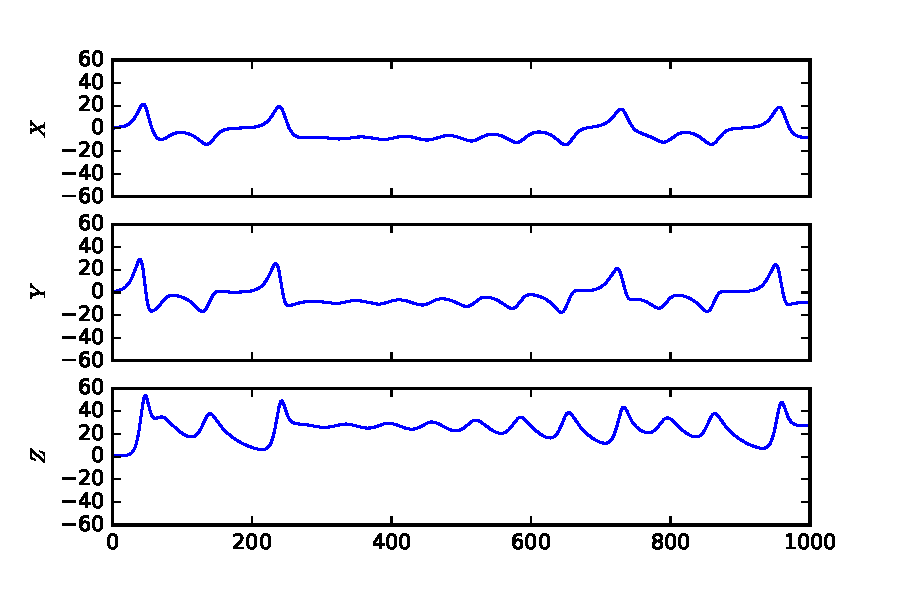
\includegraphics[width=\linewidth]{figures/lorenz_series.pdf}
		\caption{Lorenz system time series}
		\label{fig:lorenz_time_series}
	\end{subfigure}
	\begin{subfigure}{0.45\linewidth}
		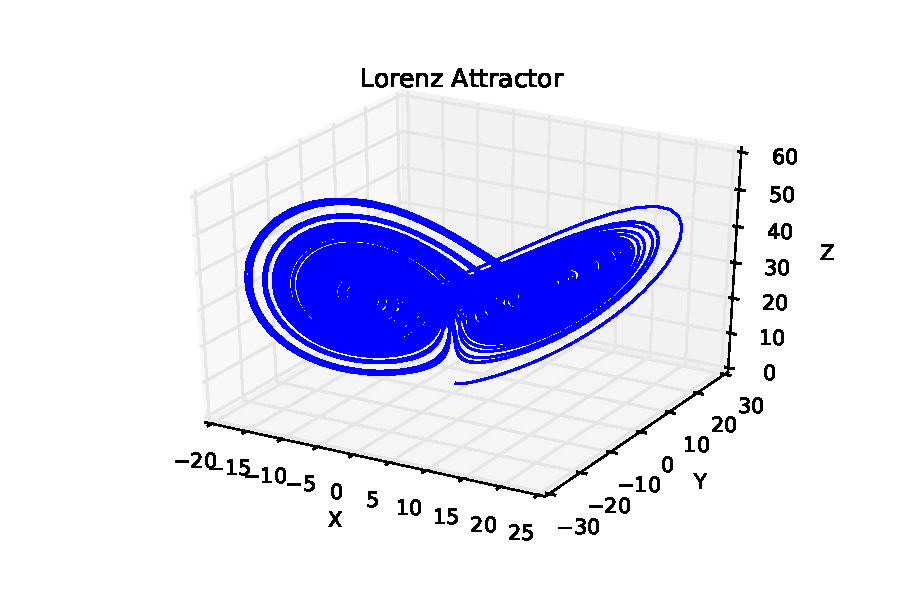
\includegraphics[width=\linewidth]{figures/lorenz.pdf}
		\caption{Lorenz Attractor}
		\label{fig:lorenz_attractor}
	\end{subfigure}
	\caption{A Lorenz system with initial conditions $x=0$, $y=1.0$, $z=1.05$, $\sigma=10$, $\rho=28$, $\beta=2.667$, and time differential of $0.01$. The series represent interlinked components in a system, and the manifold is made up of all the three series combined. The manifold is constructed by mapping the combination of $x$, $y$, and $z$ at each unique time point to a coordinate in an $n$-dimensional space, where $n$ is the number of components---$n=3$ in this case. The resulting mathematical $n$-dimensional object is called a manifold, and can be used to describe the state of the system in terms of complexity, flux, and stability. In this given example, it can be seen that the system gravitates towards two main "loops", and therefore the system is \textit{attracted} to those points in the three dimensional space.}
	\label{fig:lorenz}
\end{figure}

\subsection{Shadow Manifolds}
A shadow manifold of time series $\omega$ is an $E$ dimensional reconstruction of $E$ delayed signals of $\omega$. For example, if our $\omega$ variable is actually the \textit{sin} function, then to construct $E$ delayed signals of $\omega$ we would calculate

\begin{align*}
	\omega_1(t) &= sin(t) \\
	\omega_2(t) &= sin(t-1) \\
	\omega_3(t) &= sin(t-2) \\
	\vdots& \\
	\omega_E(t) &= sin(t-(E-1)) \\
\end{align*}

and then to construct a shadow manifold of $\omega$ we would construct a manifold of $\omega_1$, $\omega_2$, $\dots$ , $\omega_E$ (Fig. \ref{fig:sin_shadow_manifold}). Since the scalar by $1$ increment seems too general, the signals are delayed by multiples of $\tau$, where $\tau$ is approximated by field knowledge or mathematical analysis. Therefore, the formal way to describe shadow manifolds is that they are signals delayed by a  scalar multiple of $E\tau$ such that shadow the manifold of $\omega$, $M_{\omega}$, is described as 
\begin{align*}
	M_{\omega} &= f\Big(\omega_1(t), \omega_2(t), \omega_3(t), \dots, \omega_E(t)\Big)\\
	&= f\Big(\omega(t), \omega(t-\tau), \omega(t-2\tau), \dots, \omega(t-(E-1)\tau)\Big)
\end{align*}


\begin{figure}
	\centering
	\begin{subfigure}{0.45\textwidth}
		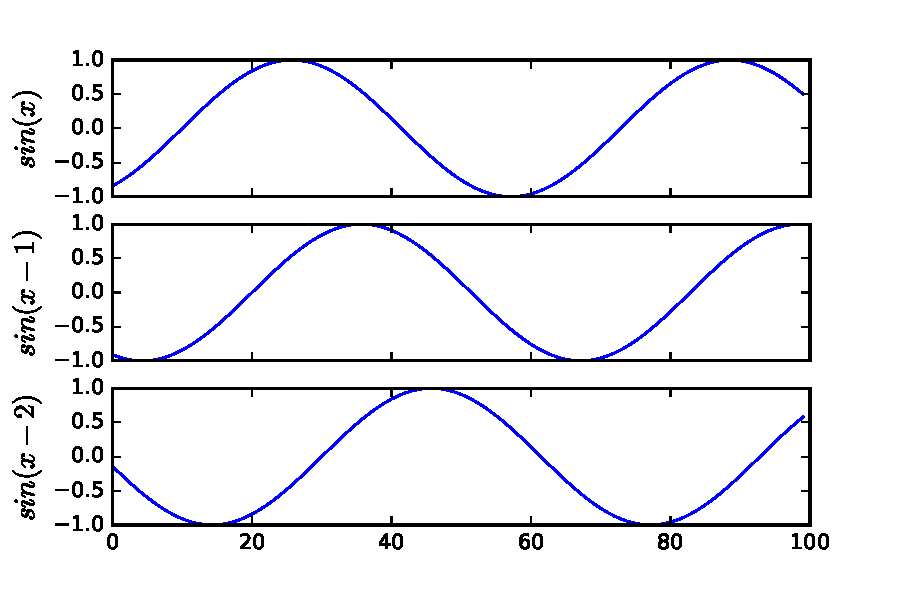
\includegraphics[width=\linewidth]{figures/sin_delayed_signal.pdf}
	\end{subfigure}
	\begin{subfigure}{0.45\linewidth}
		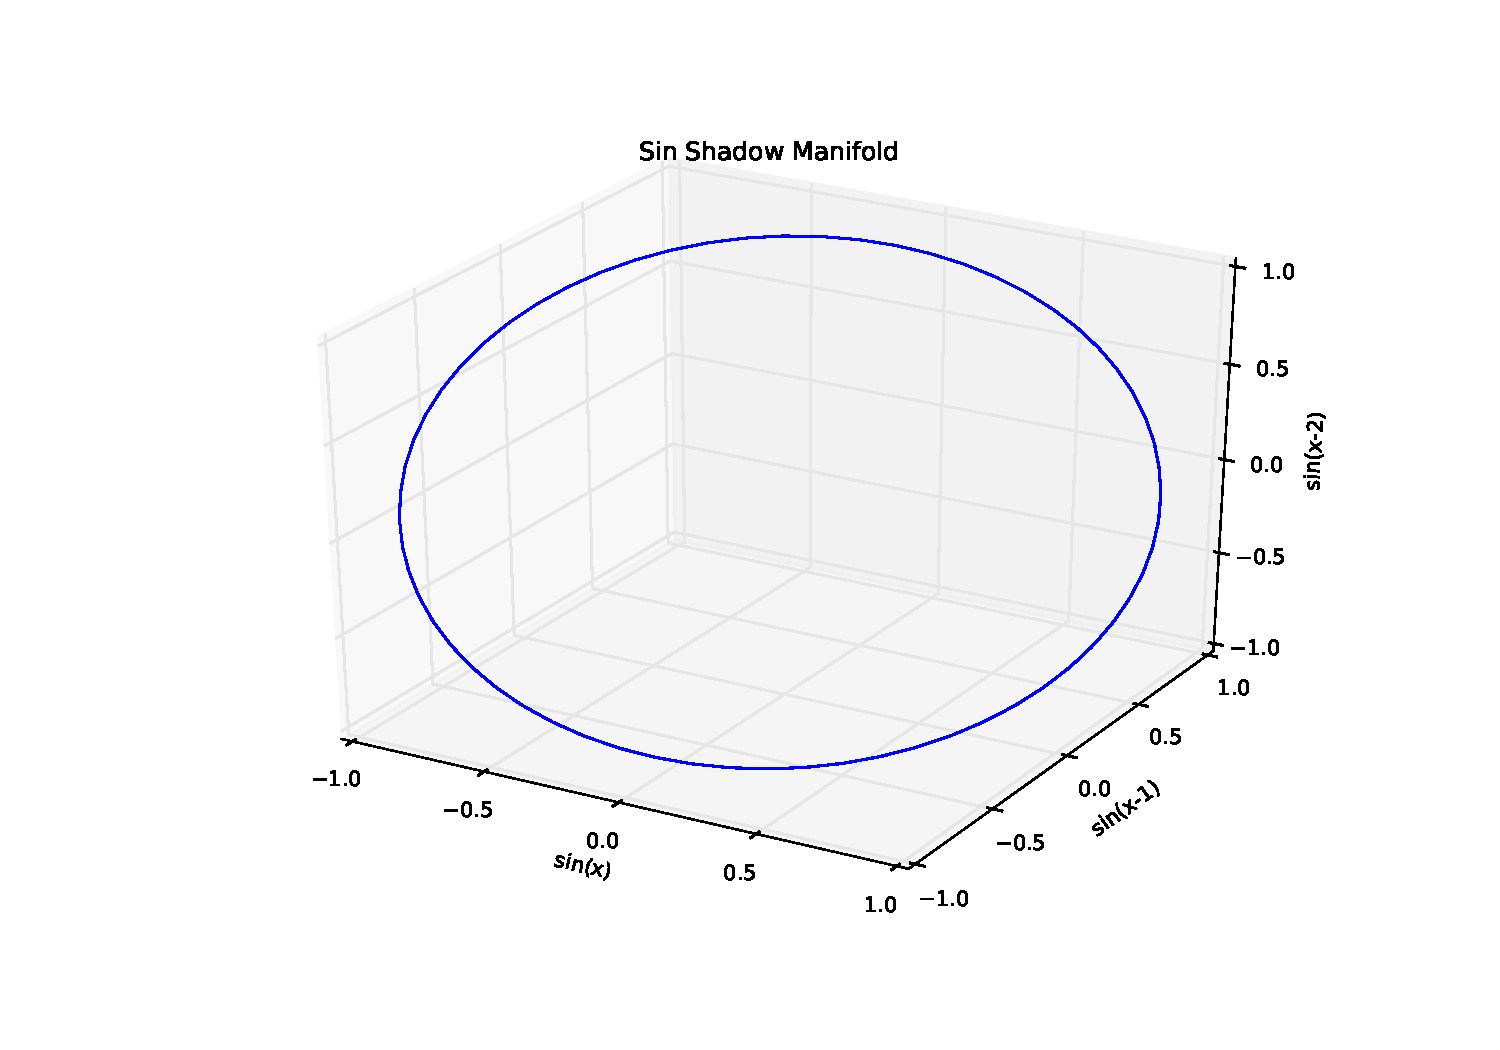
\includegraphics[width=\linewidth]{figures/sin_shadow_manifold.pdf}
	\end{subfigure}
	\caption{A shadow manifold of a simple sin function. The delayed signals are created by delaying the series by a scalar constant $\tau$ (in this case $\tau=1$ and $E=3$ so the function is delayed by $1,2,3$). From these delayed signals, a manifold is constructed by mapping each time point of all the delayed signals to an $E$-dimensional manifold called a shadow manifold.}
	\label{fig:sin_shadow_manifold}
\end{figure}


By using a theorem called Takens' embedding theorem, it can be shown that each shadow manifold of a variable is a projection of the dynamic system's manifold, $M$, that preserves the topology of $M$ \cite{Dixon1999,Deyle2011,Takens1981}. For example, in a dynamic system like the Lorenz Attractor where the dynamics of each variable is affected by the other variables in the system, it can be said that each variable subscribes to the overall dynamic of the system. Therefore, the state of one variable could be used to infer the state of another variable if they are dynamically linked. A visual demonstration of this can be seen in Figure \ref{fig:lorenz_topology} where the shadow manifold of each of the variables in the Lorenz system maintains part of the topology of the original whole system. This important property of shadow manifolds imply that there is a one-to-one relationship between a shadow manifold and the original system manifold. More importantly, this also implies that there is a one-to-one relationship between the shadow manifold of one variable and each of the other shadow manifolds in the system. Therefore, the relationship between each shadow manifold is strong. A great demonstration of this concept can be viewed in the online (Science) version of the original paper by Sugihara \cite{Sugihara2012} where a video is present to elegantly describe this concept (for ease of access, the reader can also refer to a youtube video called "Takens' theorem in action for the Lorenz chaotic attractor" \cite{TakensYoutube2012}). 

\begin{figure}
	\centering
	\begin{subfigure}{0.30\textwidth}
		\centering
		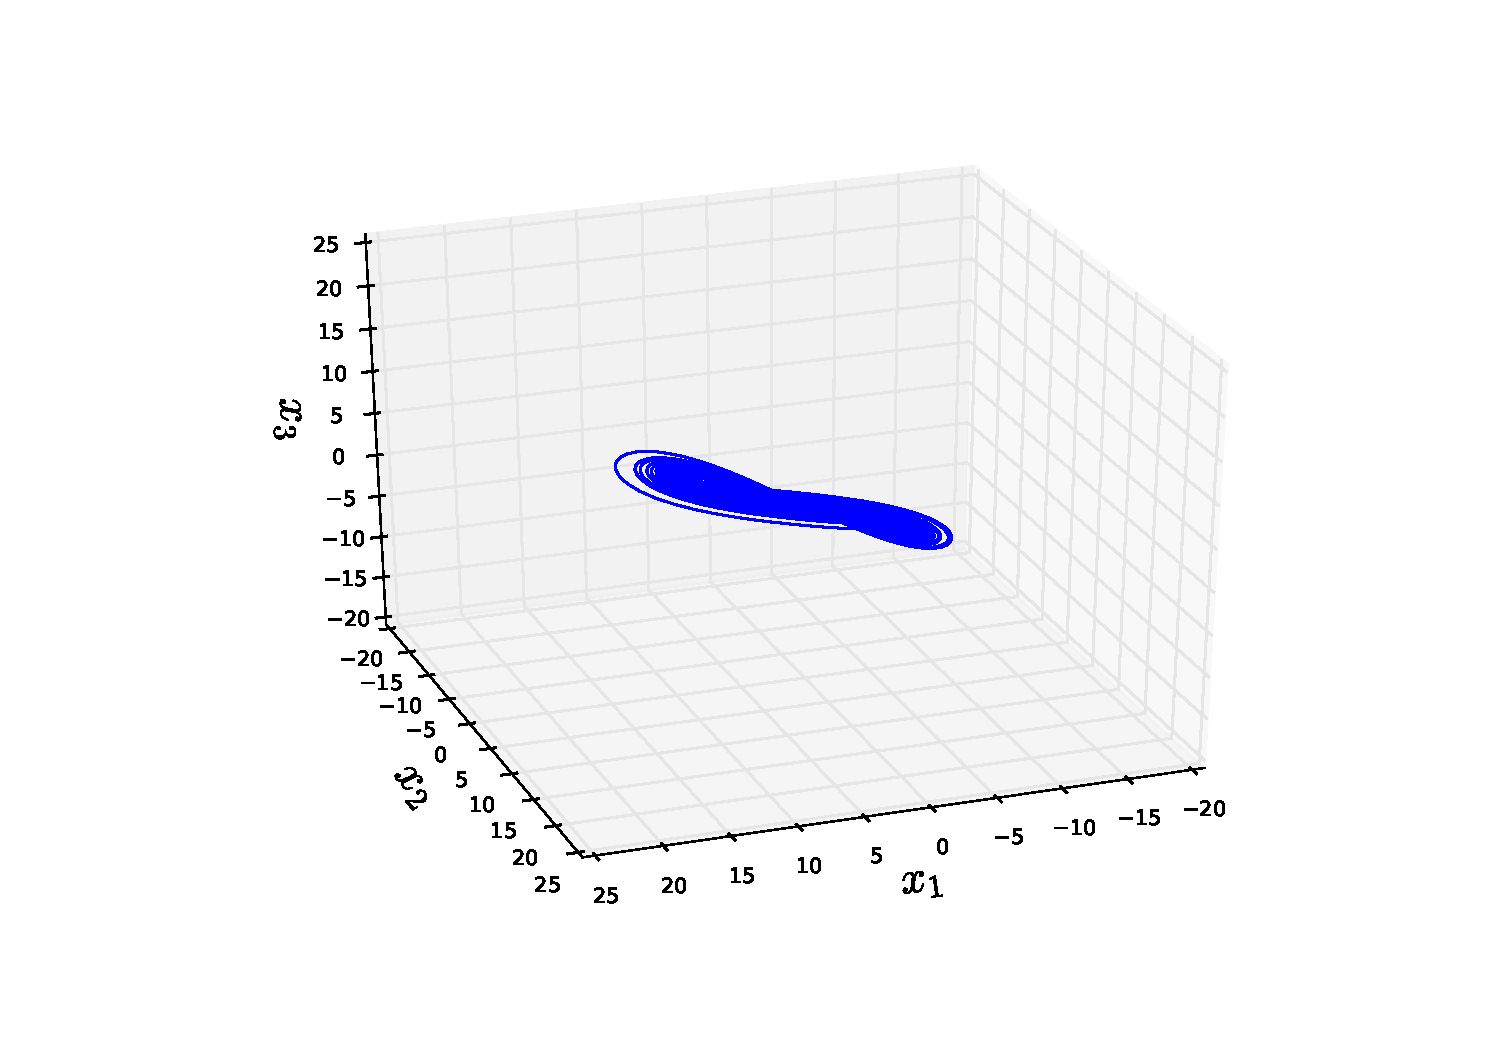
\includegraphics[width=\linewidth]{figures/shadow_manifold_x.pdf}
	\end{subfigure}
	\begin{subfigure}{0.30\textwidth}
		\centering
		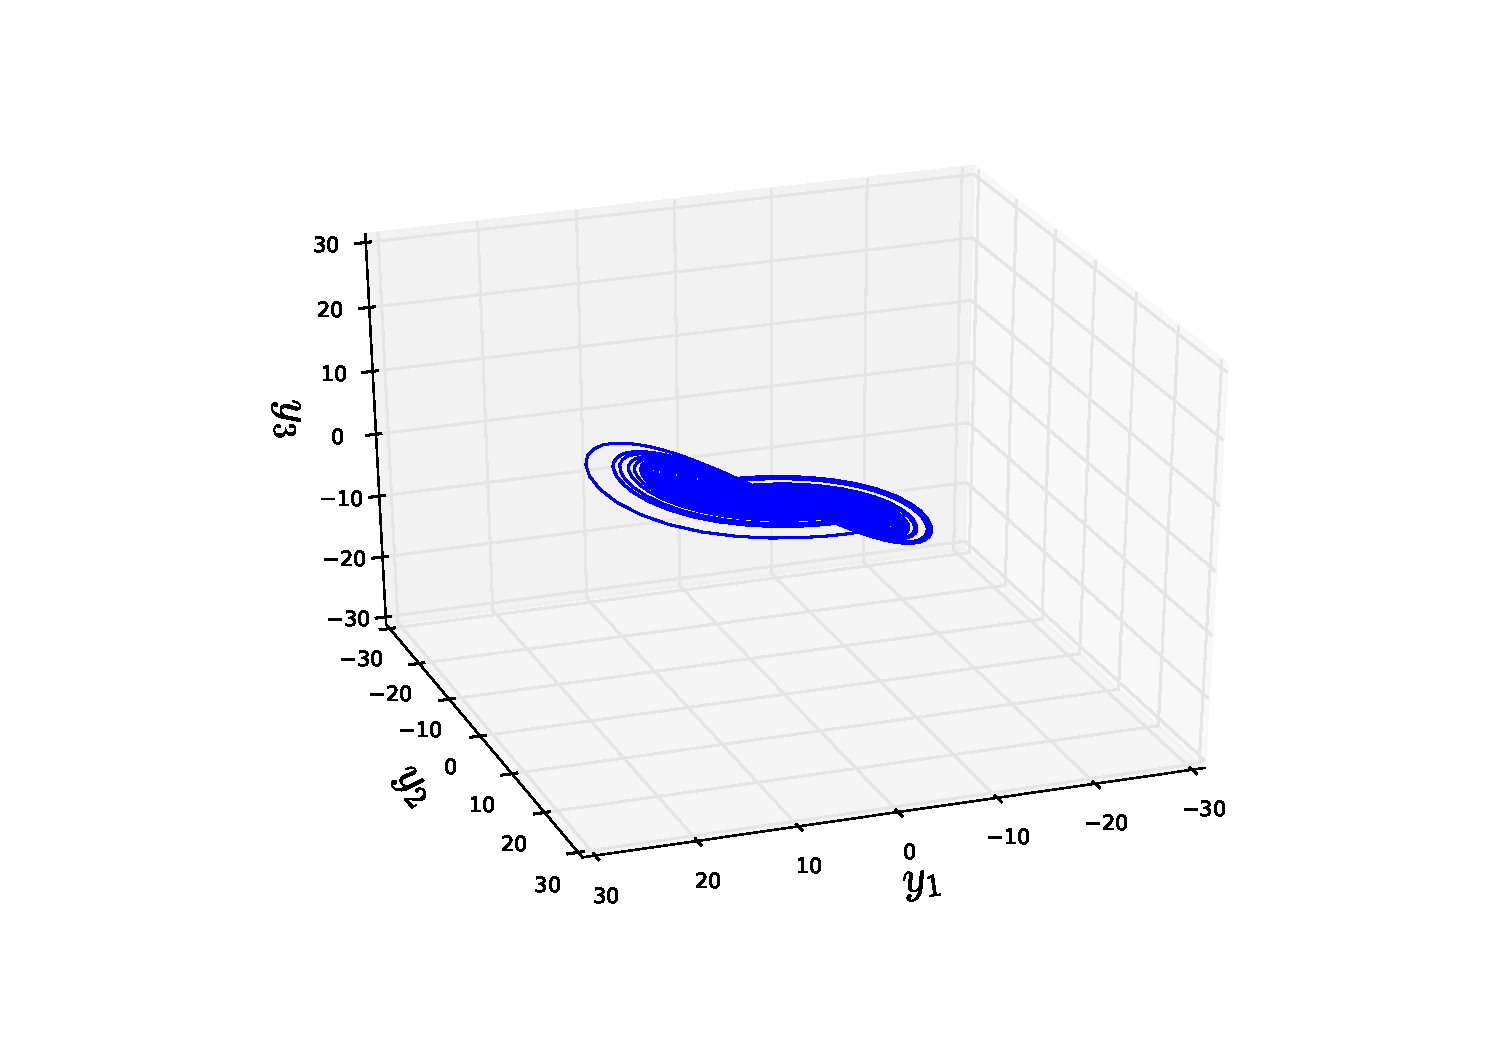
\includegraphics[width=\linewidth]{figures/shadow_manifold_y.pdf}
	\end{subfigure}
	\begin{subfigure}{0.30\textwidth}
		\centering
		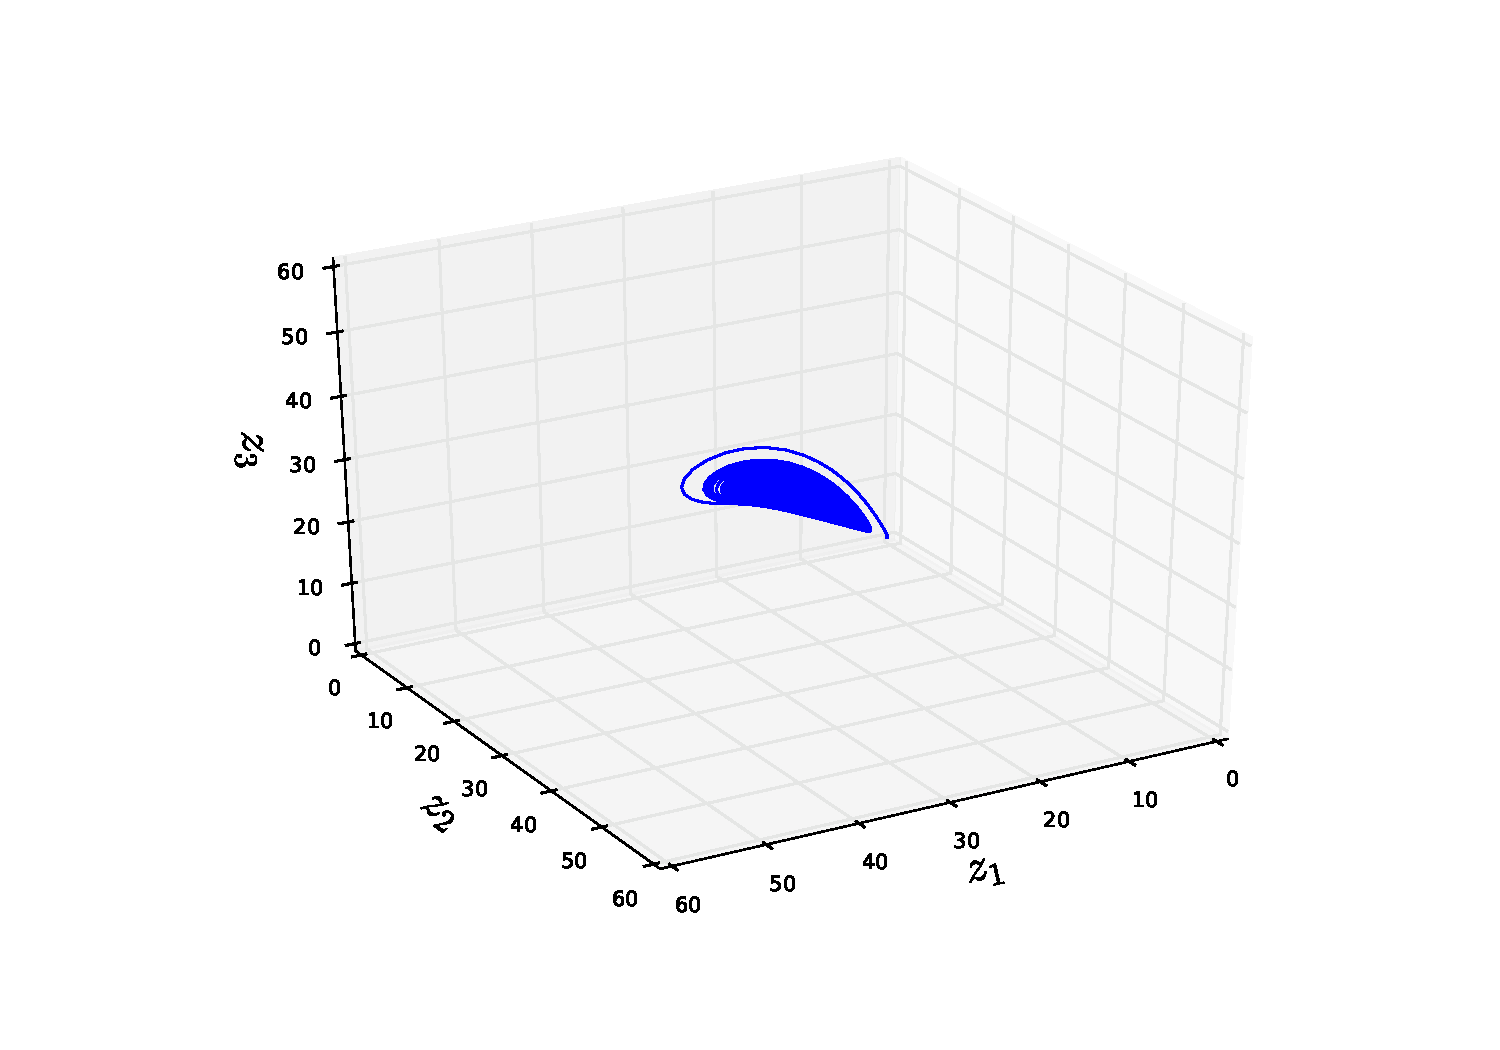
\includegraphics[width=\linewidth]{figures/shadow_manifold_z.pdf}
	\end{subfigure}
	\caption{The shadow manifolds of variables $x$, $y$, and $z$ in the Lorenz system. Each of the shadow manifolds retains part of the topology of the original system, as proven by Takens' theorem \cite{Takens1981}.}
	\label{fig:lorenz_topology}
\end{figure}

Using this relationship between shadow manifolds, the Sugihara Causality is calculated as the distance between points of similar time point on each shadow manifold. For variables $x$ and $y$, the causality at time $t$ is calculated as a measure of the time difference between closest neighbors of $y_t$. This concept is called cross-mapping, and is illustrated in the supplemental materials on the original paper, and the youtube video referred to previously \cite{Sugihara2012, TakensYoutube2012}. The last portion of the Sugihara model is the Convergent in Convergent Cross Mapping, which refers to the convergence of the causality value (cross mapping score) when the library of reference points in $x$ and $y$, $L$, is considered. The library $L$ simply refers to the specific range of $x$ and $y$ values to be used in the cross mapping calculation. For example, $L$ could be 20, which means only 20 time-synced data point observations of $x$ and $y$ are taken into consideration, or it could be $100$, which means 100 $x$ and $y$ variables are considered. The Sugihara model expects for a causal relationship to \textit{converge} to a value as $L$ increases. This implies that $L$ needs to be sufficiently large to allow an observation of convergence. This convergence is the test used to determine Sugihara Causality, named after its author who describes it as a required but not complete definition of causality \cite{Sugihara2012}. This approach is the first step towards more general and applicable causality models since Granger Causality. Since the introduction of Convergent Cross Mapping, it has been shown to be successfully predictive in biological \cite{Deyle16042013,Wang2014,Sugihara2012,Mcbride2015,Nes2015} and cosmological \cite{Tsonis2015} applications while showing weaknesses in others \cite{Mccracken2014}. 

Extensions to and amalgamations of the CCM model are beginning to surface in literature. Clark \textit{et al.} proposed an extension to CCM that relies on measuring the smoothness of the mapping (also called flow) function $\phi$, thereby reducing the $L$ length requirement\cite{Clark2015}.  Wismüller \textit{et al.} proposed a Mutual Connectivity Analysis framework for the "analysis and visualization of non-linear functional connectivity in the human brain from resting state functional MRI" \cite{wismuller2014} which relies heavily on CCM. Tajima \textit{\textit{et al.}} use the fundamental idea of state space reconstruction to find two measures. The first is \textit{Complexity} which is the best embedding dimension for a certain signal (embedding dimension at which the cross mapping is saturated). The second is \textit{directionality}, the difference in cross map skill or embeddedness between two a pair of signals. With those two measures, they show that the brain exhibits different complexities during conscious and unconscious states. Here, we explore the application of CCM in estimating the causality between neuronal regions by constructing a network of pairwise causality. We then analyze features of such networks during normal and epileptic seizure periods, and use this in conjunction with machine learning to observe if Sugihara Causality can unearth modes of communication in the brain.


\section{Experiment}
\subsection{Problem Statement}
Given multiple EEG signals from a set of interconnected neuronal regions, can the CCM model identify structural patterns in causal relationships between those regions? Can the patterns and properties of the causality graph resulting from the CCM model be clustered into brain states that represent different stages of epilepsy in the brain? In other words, can a machine learning algorithm be applied to the causal network properties, the model of which could be able to correctly classify epileptic brain states.

\subsection{Methods}
\subsubsection{Data Collection}
EEG data was collected from an 4x8 endodermal electrode array at a frequency of 1000 Hz (31 channels, one channel malfunctioned, Fig. \ref{fig:rat_experiment}). The data recording lasts for ~500 seconds, during which epileptic seizures were evoked using 4-aminopyridine and EEG data was recorded from the electrode array. The spiking voltage of each recorded electrode is used as a signal and is referred to as a channel (Fig. \ref{fig:example_eeg_and_kcsd}). Each channel has a continuous data series that spans the 500 seconds.

\begin{figure}[H]
  \centering
  \begin{subfigure}[b]{0.45\textwidth}
    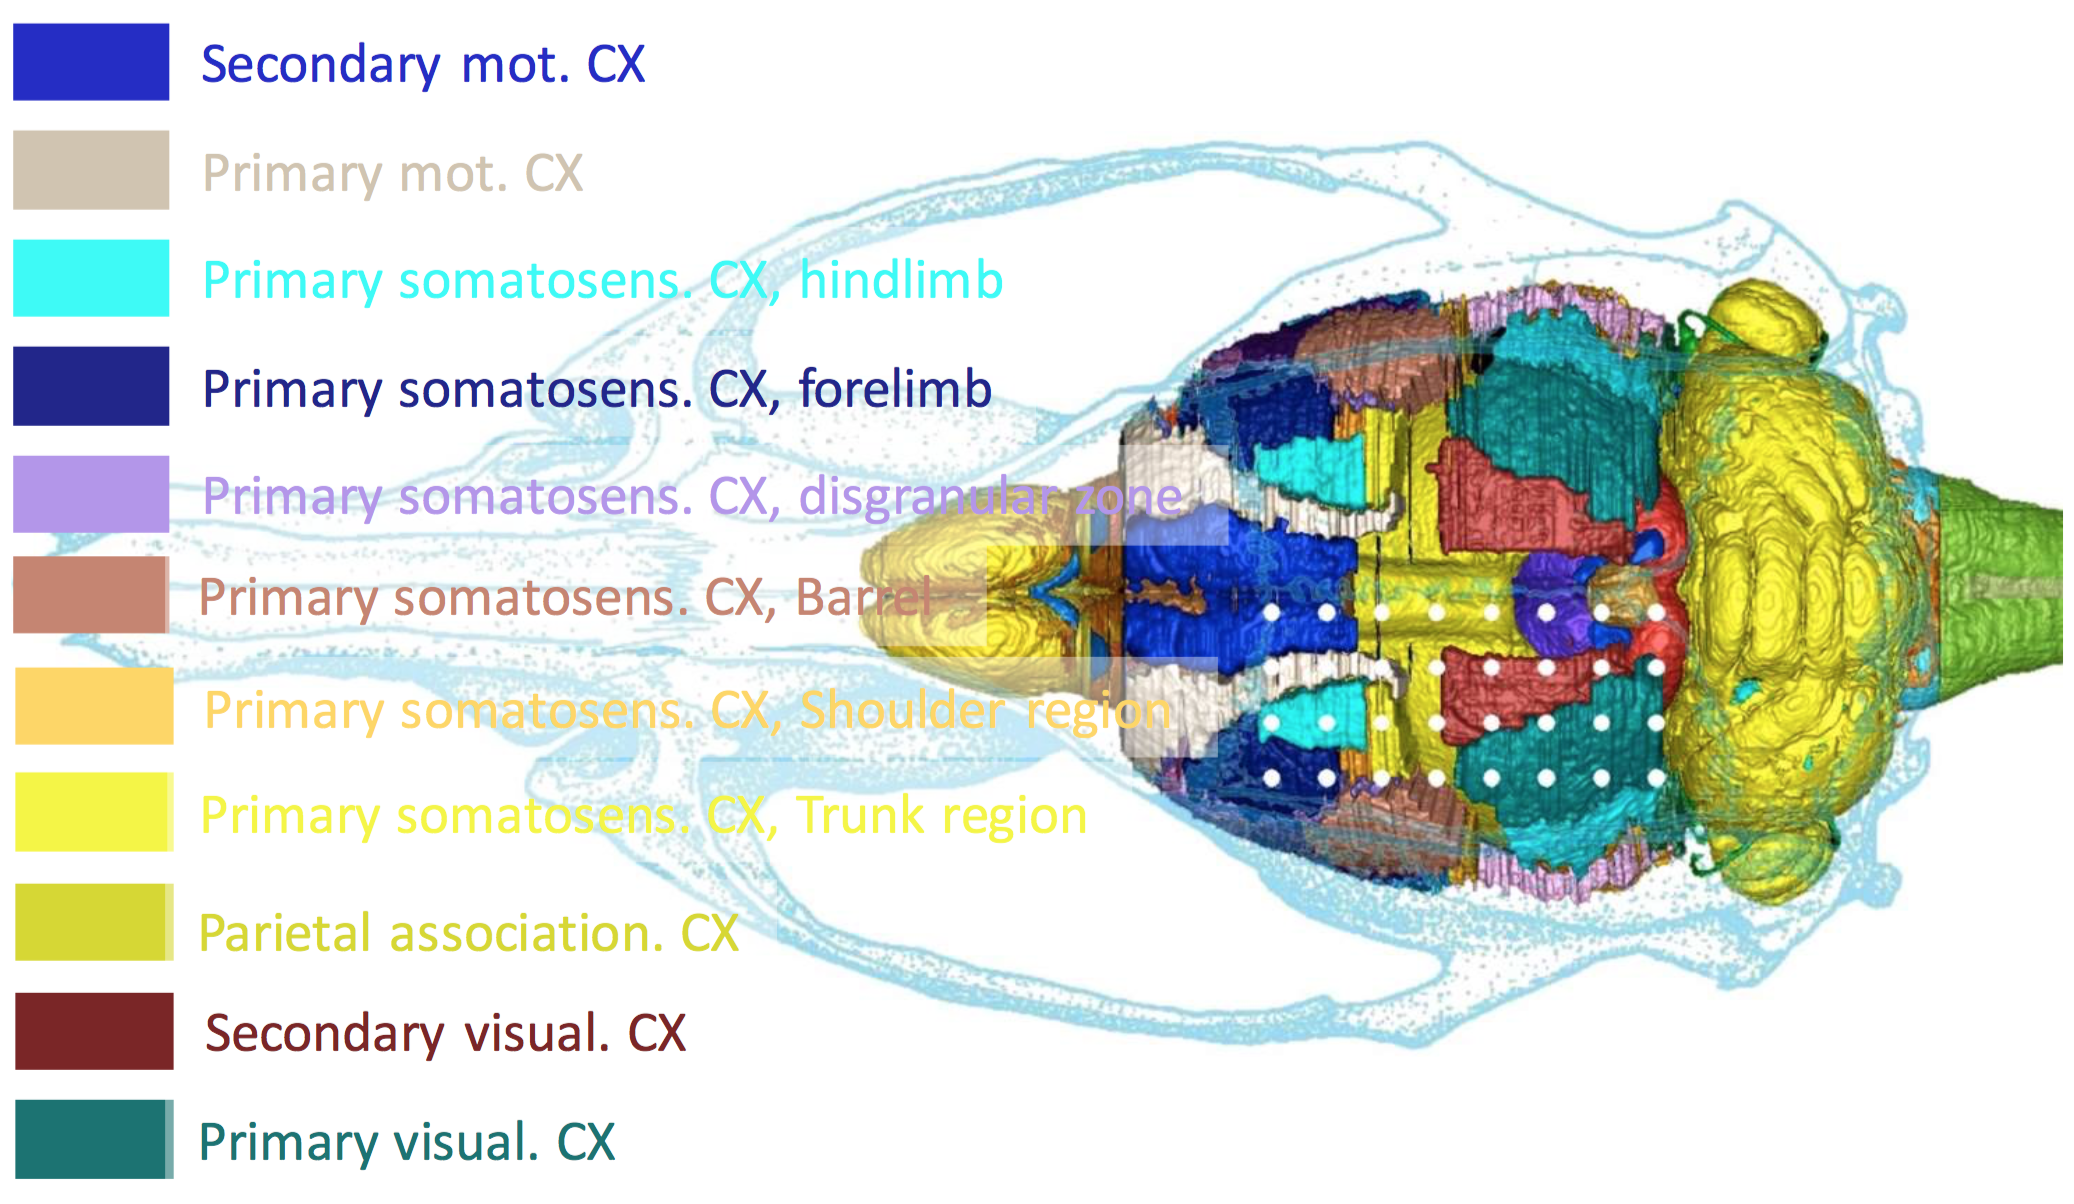
\includegraphics[width=0.95\linewidth]{figures/rat_brain_schematic.png}
    \caption{}
  \end{subfigure}
  \begin{subfigure}[b]{0.45\textwidth}
    \centering
    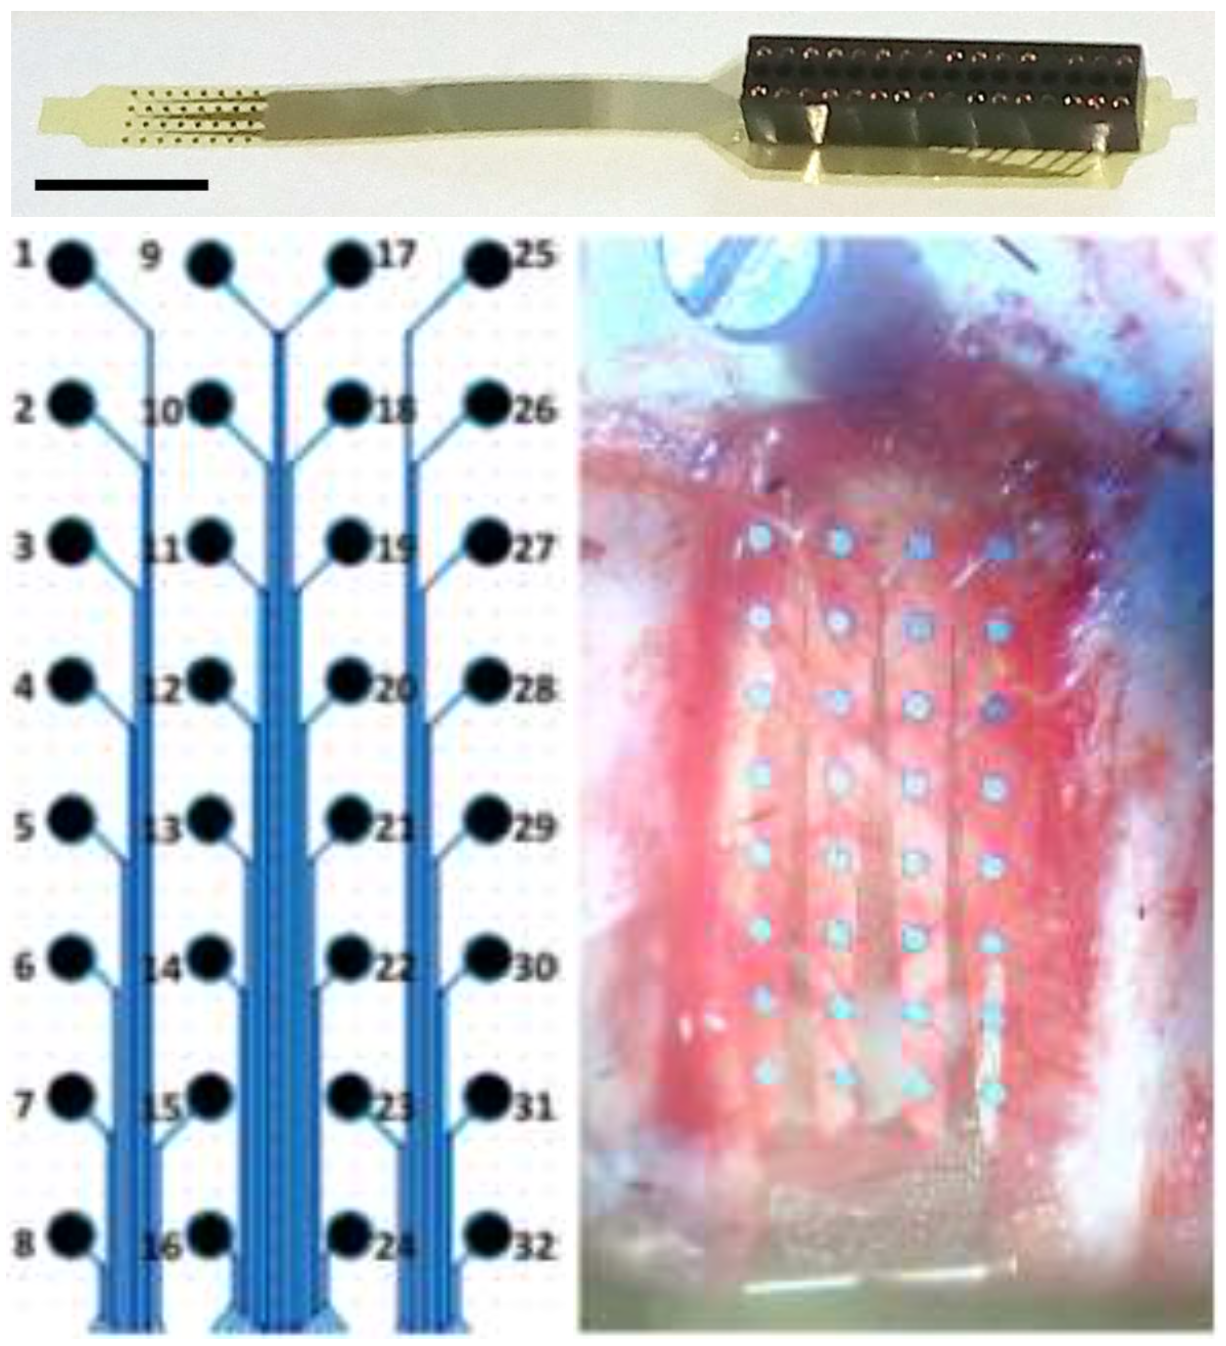
\includegraphics[width=0.95\linewidth]{figures/rat_scull_and_instrument.png}
    \caption{}
  \end{subfigure}
  \caption{(a) A composite drawing showing the brain in the scull. The 3D reconstruction of the brain has been made using the maps of the Paxinos atlas, and the localization of cortical areas are indicated by different colors. White points indicate the position of the recording sites of the membrane electrode. Names for the cortical areas are also shown (based on Hjornevik \textit{et al.} and Paxinos \textit{et al.} \cite{hjornevik2007} \cite{paxinos2009}). (b) Photograph of a membrane electrode shows the construction on the top, the numbering (bottom right) and the surgical implantation (bottom left) is also shown. Electrode 1 malfunctioned during recording.}
  \label{fig:rat_experiment}
\end{figure}


\begin{figure}[H]
  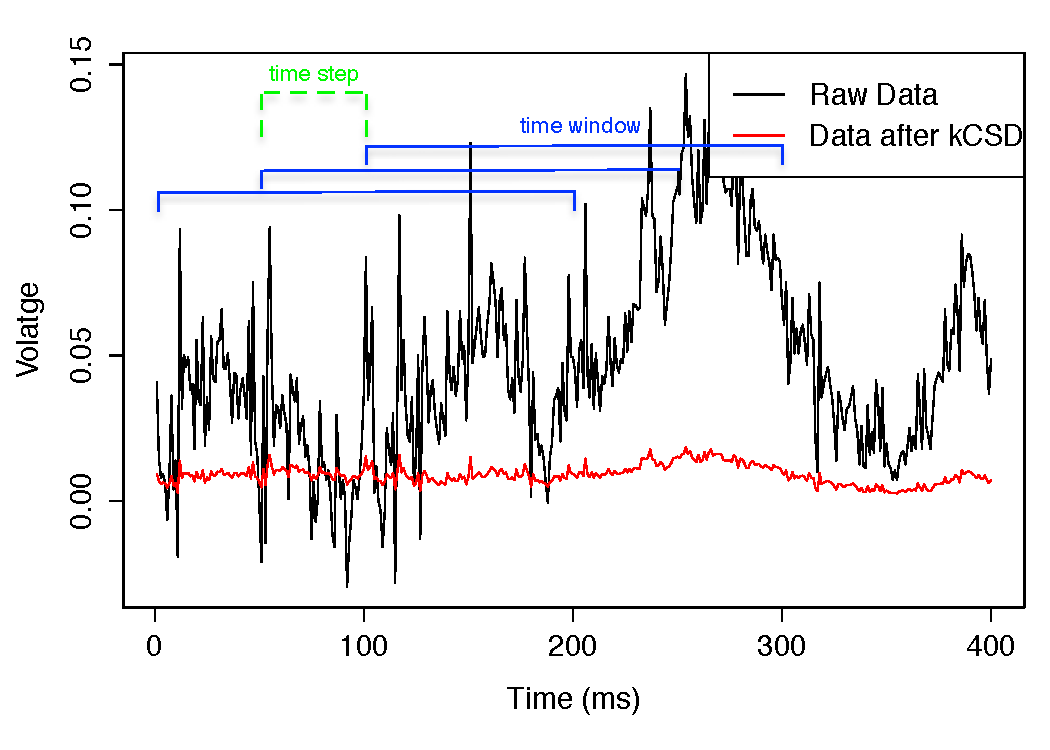
\includegraphics[width=\linewidth]{figures/sample_eeg_signal_with_kcsd_edited.pdf}
  \caption{Sample data from electrode 1, in both its raw form and then in its form after kCSD transformation. Applying kernel Current Source Density extracts the true relationship of neural activity, and in theory eliminates disturbances that might be caused by signal interference. Three sample blue lines are drawn to demonstrate the sliding windows that were used to calculate Sugihara Causality between brain regions. In each time window, the causality was calculated between each brain region, and the time window was moved by an amount \textit{time step}. Different configurations were used for the time window and time step, as reported in table \ref{tab:sliding_window_configuration}. Here, the configuration shown has time window as $200$ and time step as $50$.}
  \label{fig:example_eeg_and_kcsd}
\end{figure}

\begin{table}[H]
\centering
\caption{Configurations used for the sliding window when calculating Sugihara causality that was used as a measure of brain communication. These configurations inform our model of the granularity of brain communication. Since we do not know exactly how quickly information is being passed down from region to region, arbitrary choices were made to test how well each performs and make a more informed decision in future research. Because we have different time steps, there are a different number of graphs (data points) in each dataset.}
\label{tab:sliding_window_configuration}
\begin{tabular}{|c|c|c|c|}
\hline
 Dataset name &  Time window &  Time step & Number of Data points\\ \hline
 
 dataset 50 & 200 & 50 & 10190 \\ \hline
 dataset 200 & 200 & 200 & 2547 \\ \hline
 dataset 250 & 2000 & 250 &  2038 \\ \hline
\end{tabular}
\end{table}

\subsubsection{EEG Data Preprocessing}
Kernel Current Source Density (kCSD) method was used on the grid of channels to account for possible electrical interference with the direct measurement (Fig. \ref{fig:example_eeg_and_kcsd}) \cite{Potworowski2012}. The measured potentials produced by kCSD arise as the linear combination of the trans-membrane currents, which is a more direct and localized quantity to measure the neural activity. Therefore current source density distribution was calculated by the kCSD method and used for the analysis instead of the original EEG signals.

Afterwards, in order to reduce the data size that is operated on, we lumped channels from the same brain regions together by averaging them (Fig. \ref{fig:brain_region_lumping}). In addition to reducing dimensionality, this process also puts emphasis of causality on functional brain regions instead of a local cluster of neurons. 

\subsubsection{Sugihara Causality Measurement}
After lumping the kCSD signals from the same region, we perform Sugihara Causality calculation on the regions by using a sliding windows method (Fig. \ref{fig:example_eeg_and_kcsd}). Because we do not know how granular of a time frame the brain uses to communicate (and how that affects the EEG signal we record), we use three different time scales as reported in table \ref{tab:sliding_window_configuration}. This produces 3 datasets with similar characteristics. The important thing to keep in mind is that after this step, each causality measure that resulted from the Sugihara Causality analysis is a measure of how much one region is affecting the other, and we use that as a way to describe brain communication and information flow. Each causality measure is therefore an \textit{edge} of communication from one region to another, meaning that each brain region is a node and each causality measure is a weighted edge. Figure \ref{fig:sample_graph} shows a sample graph constructed from joining all the causality measures from a specific time window. This is essentially a (theoretical) snapshot of how each brain region was affecting other brain regions in that time window.

\begin{figure}[H]
  \centering
  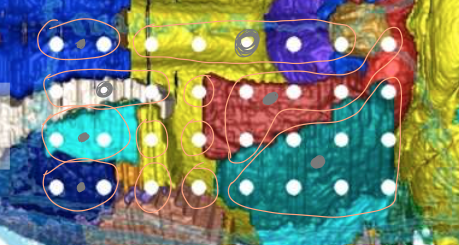
\includegraphics[width=0.65\linewidth]{figures/brain_region_lump.png}
  \caption{The distribution and lumping of the brain regions in the brain. A total of 12 region channels were constructed from the initial 31 local channels. The schematic is based on rat brain atlas mapping.}
  \label{fig:brain_region_lumping}
\end{figure}


\begin{figure}[H]
  \centering
  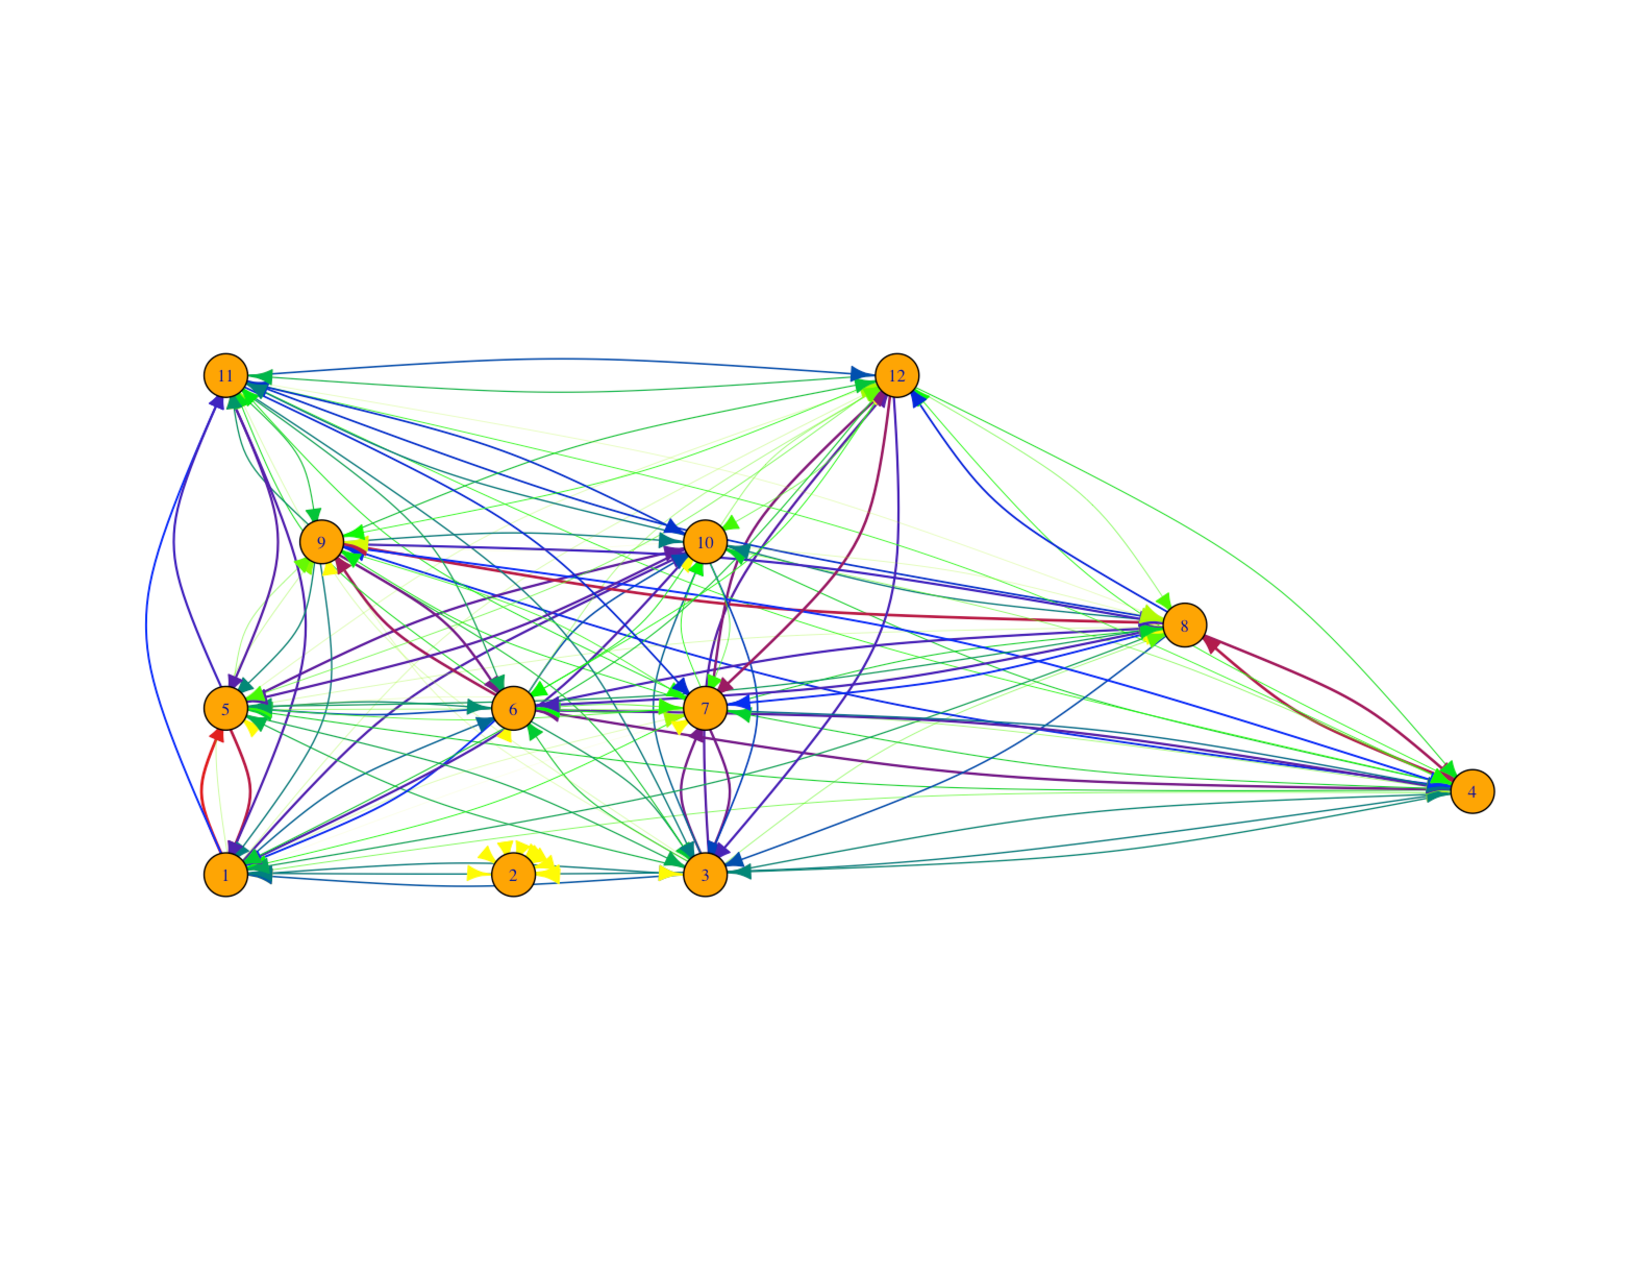
\includegraphics[width=0.55\linewidth]{figures/sample_graph.pdf}
  \caption{Sample graph constructed from calculating the Sugihara causality between brain regions. Lumped brain regions correspond to the gray circular mapping in Fig. \ref{fig:brain_region_lumping}. Edge colors represent the strength of the causal relationship. From weakest to strongest: Yellow, Green, Blue, Red. The edge weight ranges from 0 to 1.}
  \label{fig:sample_graph}
\end{figure}


\subsubsection{Data Exploration and Visualization}
The data we produced is a series of complete, directed graphs (all the same topology; each node is a brain region as seen in figure \ref{fig:rat_experiment}; each edge is a causality/communication measure) and their edge weights that we refer to as $\rho$ scores ($\rho$ is the convention name for the score of a Sugihara Causality analysis). Since we processed the data with different time steps, there are a different number of graphs available in each dataset (Tab. \ref{tab:sliding_window_configuration}). For each graph, there are $132$ $\rho$ scores, all of which range between 0 and 1 (decimals). Each graph was transformed into a vector where each vector is a data point, and all vectors make a dataset. This transformation was required for the data to be entered into sklearn's Gaussian Mixture model function properly.

In all graphs, most of the $\rho$ scores appear to be of high values, suggesting high connectivity between brain regions and therefore a high density graph (Fig. \ref{fig:rho_hist_all_experiment}). This indicates that there is constant information flow between regions in the brain. Furthermore, we also notice that many of the $\rho$ scores to be similar within a pair of nodes (Fig. \ref{fig:diff_within_pair_hist}). For example, when looking at regions 1 and 2 within the first 200 milliseconds, they appear to be equally communicating to one another (Fig. \ref{fig:sample_pair_causality_plot}). This could be indicative of either bidirectional causality or unidirectional forcing, both of which can be detected by the Sugihara model.

\begin{figure}[H]  
  \centering
  \begin{subfigure}{0.45\textwidth}
    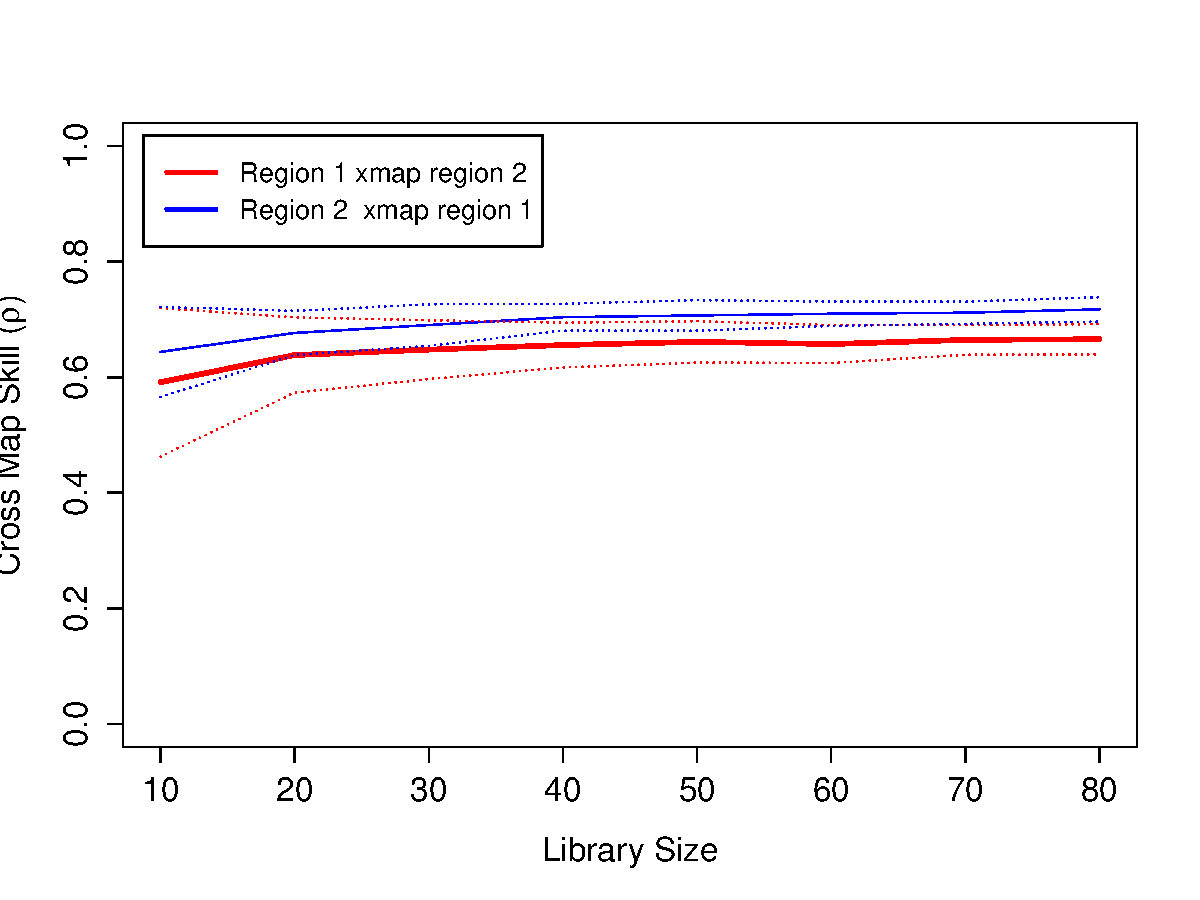
\includegraphics[width=\linewidth]{figures/sample_pairwise_causality_measure.pdf}
    \caption{}
    \label{fig:sample_pair_causality_plot}
  \end{subfigure}
  \begin{subfigure}{0.45\textwidth}
    \centering
    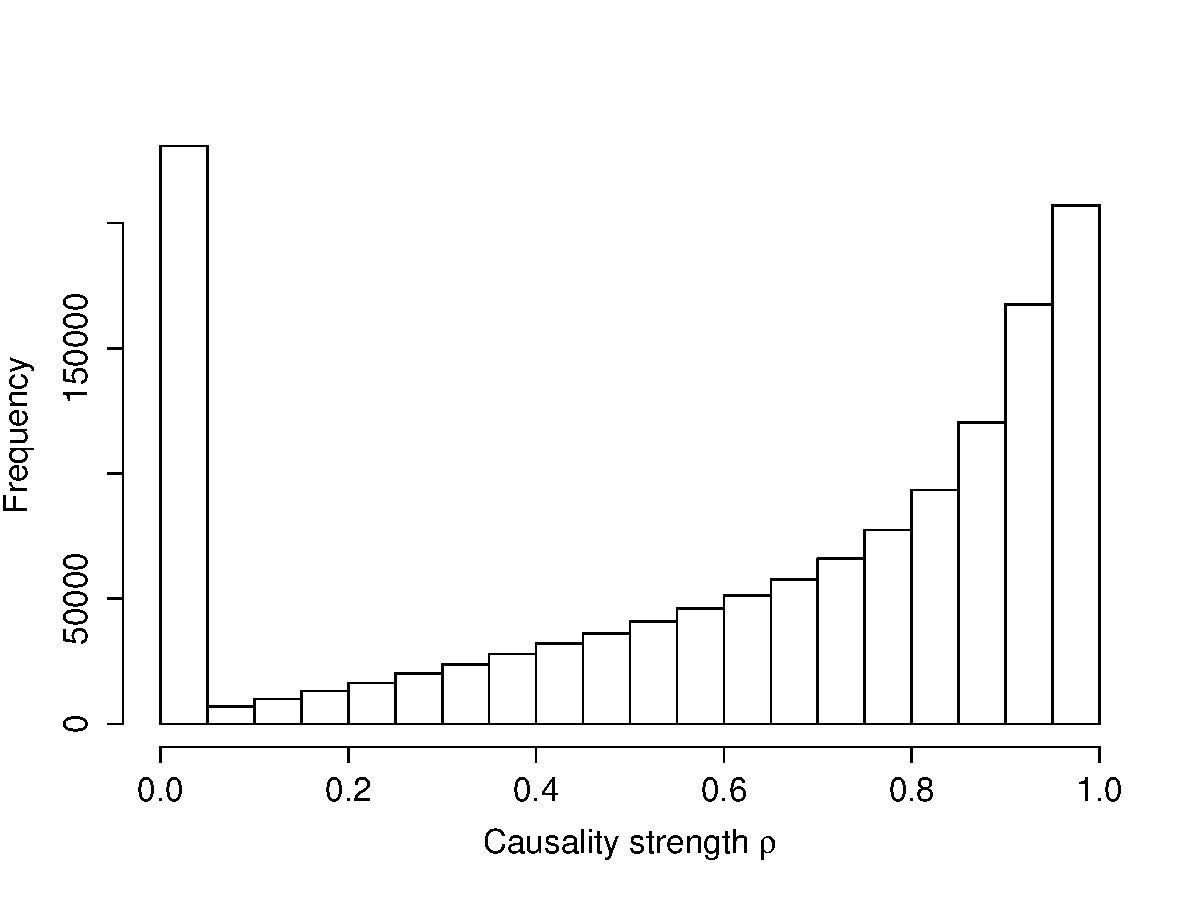
\includegraphics[width=1\linewidth]{figures/rho_hist_all_experiment.pdf}
    \caption{}
    \label{fig:rho_hist_all_experiment}
  \end{subfigure}
  \caption{(a) A sample graph plotting the convergent cross mapping skill ($\rho$) between region (nodes) 1 and 2 during the first 200 ms of the experiment. The skill mapping channel 1 to channel 2 is very similar to the one mapping channel 2 to channel 1. This might infer either bidirectional causality or unidirectional forcing. A similar pattern (close $\rho$ value between pairs) was found for most of the pairs of edges. (b) The distribution of CCM skill ($\rho$) during the entire experiment. Many relationships appear to be causal in the brain, with equally as many being non-causal throughout the experiment. Causality was calculated from signals of lumped regions after calculating the CSD. Cross mapping was done on every pair of regions with library size of 80, and each pair has two causality directions. Sliding windows of 200 ms were used, with a sliding step of 50 ms.}
\end{figure}

\begin{figure}[H]
  \begin{subfigure}{.48\textwidth}
    \centering
    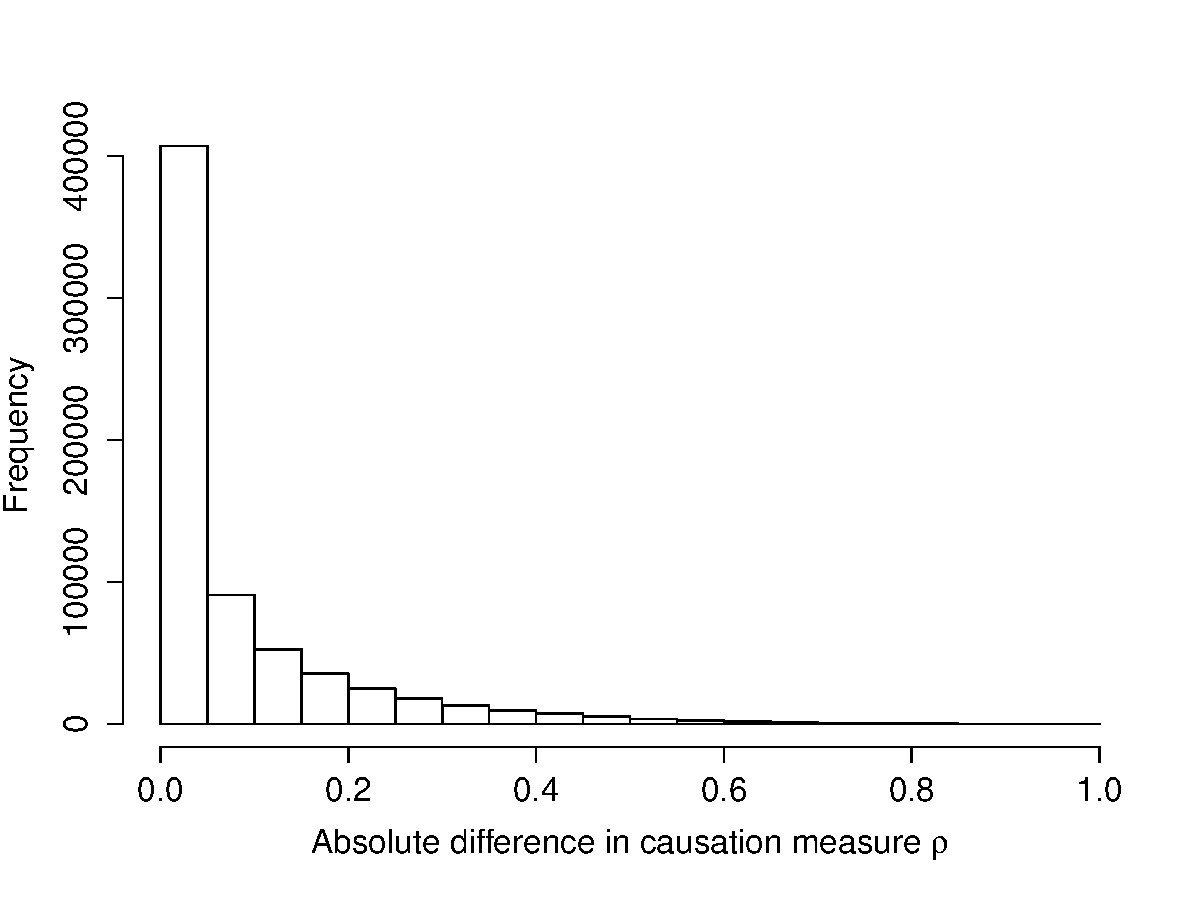
\includegraphics[width=0.95\linewidth]{figures/diff_within_pair_hist.pdf}
    \caption{Absolute difference of $\rho$ between all pairs}
  \end{subfigure}  
  \begin{subfigure}{.48\textwidth}
    \centering
    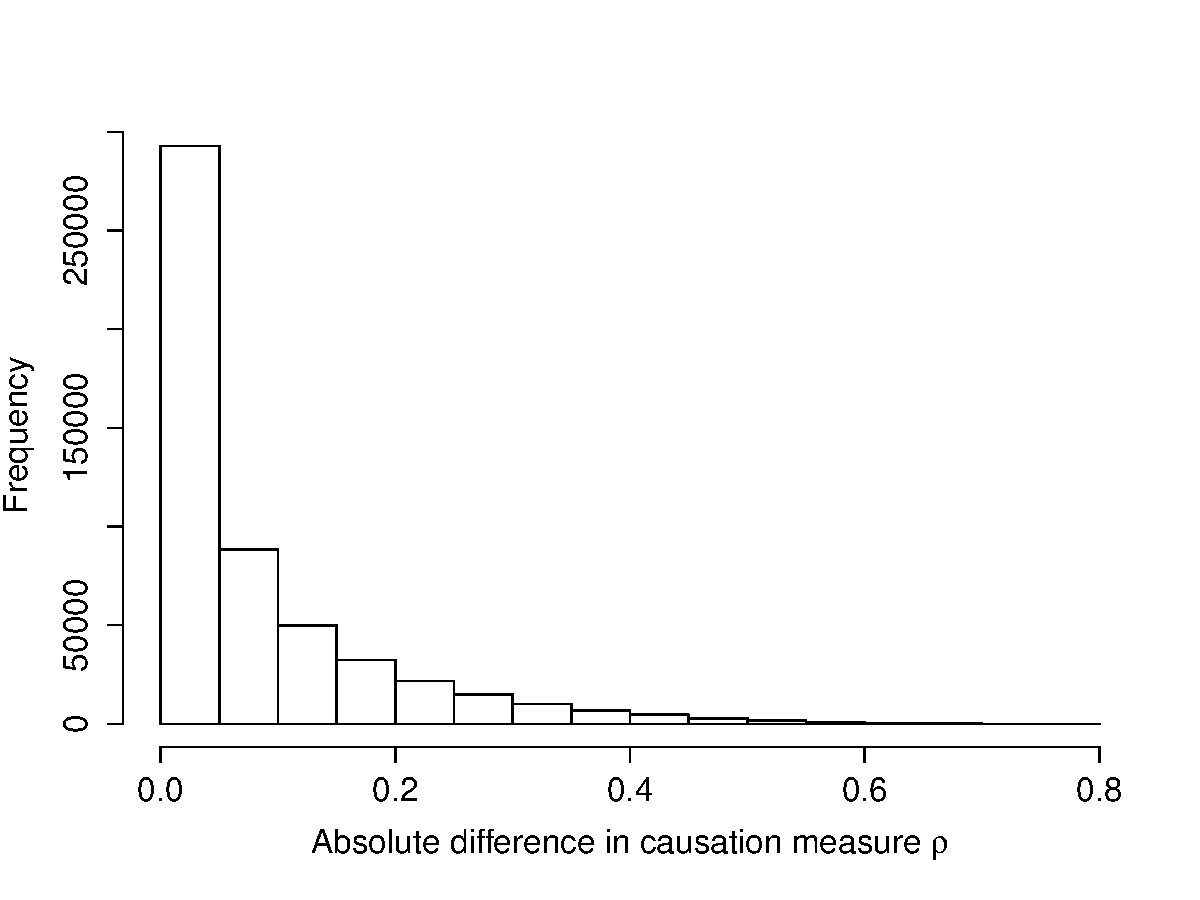
\includegraphics[width=0.95\linewidth]{figures/diff_within_pair_over_2_hist.pdf}
    \caption{Absolute difference of $\rho$ between pair both of which is at least 0.2}
  \end{subfigure}
  \caption{Difference of causality values within a pair is small, even when accounting for non-existing relationships where both causalities are below 0.2. This similarity between directions of causality in a pair could imply a bidirectional relationship between most regions, or could alternatively imply a unidirectional forcing (synchrony) phenomenon. Sliding windows of 200 ms were used, with a sliding step of 50 ms. A library size of 80 was used.}
  \label{fig:diff_within_pair_hist}
\end{figure} 


\subsubsection{Algorithms and Techniques}
The machine learning algorithms we use in this experiment are all centered around unsupervised learning, specifically clustering using an altered version of K-means called the Gaussian Mixture model. K-mean algorithms require as input a number $n$ of clusters to find, and a set of data points on which the clusters are to be found. The algorithm then works by choosing $n$ random points in the data set and setting them as centers of the clusters. Each data point that is not a center then becomes in the cluster of the nearest center. The centers are then incrementally reassigned to be the mean of the points in the clusters. This method converges in finite time to a solution, and most of the time (depending on the random initialization) finds good clusters that are well separated and in which each cluster has data points that share common features. 

Here, we choose the Gaussian Mixture algorithm as implemented by the Sci-kit learn python library instead of the simple K-means algorithm. Gaussian Mixture Model (GMM) clustering can be thought of as a K-means algorithm that is generalized to account for the covariance of the data and centers of the Gaussian distributions. Because of this feature, while K-means algorithm only clusters data points in spherical shapes, the GMM model allows clusters to take many shapes as described below under the name covariance type. For these reasons, the GMM would be a more suitable algorithm to use in our case. GMM has a few parameters that could be tuned, the most important of which is the covariance type (full, tied, diagonal, or spherical) which dictates how the cluster edges are expanded and how the clusters grow. This parameter will be fine tuned using grid search. 

Furthermore, we use Principal Component Analysis (PCA) to reduce the dimensionality of the dataset. This reduction is important because we have 132 features, and reducing them would result in a simpler analysis of the dataset. PCA works by finding the $n$ axes of most variance in the dataset and transforming the dataset into a space of only these axes. This essentially describes the dataset in a new, lesser set of dimensions than the original dimensions.

Another algorithm that is used is Grid Search, used for fine tunning the Gaussian Mixture model. The grid search algorithm is much simpler than the previous algorithms, since all it does is try to create a model with different parameters and scores each model using a given scoring function. The grid search object then ranks the models based on their scores, and can be used to retrieve the best parameters (the ones that produce the highest score).

\subsubsection{Metrics and Benchmark}
\label{sec:benchmark}
The unsupervised learning used here along with the high dimensionality of the dataset used in this experiment bring with them a unique difficulty in terms of defining a clear scoring method. In the python library we used for analysis (scikit-learn), there are only two methods that can be used to give a score to clusters (assuming no knowledge of \textit{true} labels of each data point): Silhouette Coefficient and Calinsky-Harabaz Index. Both scores ascertain the quality of clustering by measuring how dense, well defined, and separated the clusters are. We are forced to use these metrics due to the nature of the data we are given, as we don't know the true labels of the data points. However, we do know the specific times of when epilepsy was induced, and since epilepsy is \textit{one} state in the brain, then we can use the time indicies for epilepsy to be the one cluster we perform an F1 metric on. The F1 score is calculated as 

\begin{align*}
  F_1 &= 2 \cdot \frac{precision \cdot recall}{precision + recall} \\
  precision &= \frac{\text{True Positive}}{\text{True Positive} + \text{False Positive}} \\
  recall &= \frac{\text{True Positive}}{\text{True Positive} + \text{False Negative}}
\end{align*}

where positive is epilepsy and negative is non-epilepsy.

Since this method has never been attempted before (using Sugihara Causality graphs to identify epilepsy), providing a succinct and complete benchmark is a difficult task. Furthermore, the clustering here is used to explore whether or not there are any extractable information from causal networks in the brain, and whether the brain communicates differently when it is suffering from epilepsy compared to when it is operating normally. Keeping this in mind, we rely on the simple F1 score to provide a simple reliability measure of how well the clustering is separating and predicting the epilepsy cluster. Since we know that epilepsy doesn't happen often in our dataset (only ~20 seconds  of epilepsy related events in our ~500 seconds dataset), we can assign the cluster with the least data points as the epilepsy one, and then measure how exclusive the epilepsy cluster is to the times when epilepsy was \textit{actually} happening by measuring an F1 score. Since our epilepsy happens for about 4\% of the dataset, then the baseline score we expect should be 96\% of accuracy and 0.99 F1 score. These scores are attained if all the data points were labeled as one (non-epilepsy) cluster.

\subsection{Implementation}
\subsubsection{Data Preprocessing}
Some of our edge weights had some Not A Numerical (\textit{NaN}) values, and those were altered to 0, which is the lowest $\rho$ score possible. Once that error was corrected and the data has been put in the graph series format, separated into the three different datasets, we perform Principal Component Analysis (PCA) to reduce the dimensionality of the datasets. This both gives us insight into what components of the graph are logically important for the model and helps decrease the time required to run our model. The results of PCA was used to create three different datasets from each dataset: a dataset that covered 80\% of the variance, a dataset that covered 90\% of the variance, and a dataset that covered 99\% of the variance. This was done to test how dimensionality reduction would affect the final clustering efforts. Furthermore, there were some edges that showed a consistent weight of 0 (for example, all edges from node 2 to node 1 were of weight 0), and having that redundant data is not helpful to distinguishing states. PCA would help us remove such unvarying features from the datasets.

 If the scoring for the reduced datasets with only 80\% of the variance is similar to the scoring of the reduced datasets with 99\% of the variance, then we use the less dimensional reduced datasets even though they give us a less accurate version of the original information. The original dimensionality of the datasets was 132 features per data point, and a list of the PCA datasets and their different variance levels with component numbers are reported in table \ref{tab:pca_datasets}. After the principal component analysis was done on the datasets, the components required to reach the threshold levels of 80, 90, and 99 percents were recorded in table \ref{tab:components_needed_for_variance} (Fig. \ref{fig:pca_analysis_variance}).


\begin{table}[H]
\centering
\caption{Dataset names for the result of PCA analysis. Three different reduced datasets are produced each of which keeps a certain percentage of the original variance. Since we started with three datasets and created three new ones out of each by applying PCA with different levels of components, we arrive at 9 total reduced datasets.}
\label{tab:pca_datasets}
\begin{tabular}{|c|c|c|c|}
\hline
  &  80\% variance &  90\% variance & 99\% variance \\ \hline
 
dataset 50 & reduced 50 80 & reduced 50 90 & reduced 50 99  \\ \hline
dataset 200 & reduced 200 80 & reduced 200 90 & reduced 200 99  \\ \hline
dataset 250 & reduced 250 80 & reduced 250 90 & reduced 250 99  \\ \hline
\end{tabular}
\end{table}


\begin{figure}[H]
  \centering
  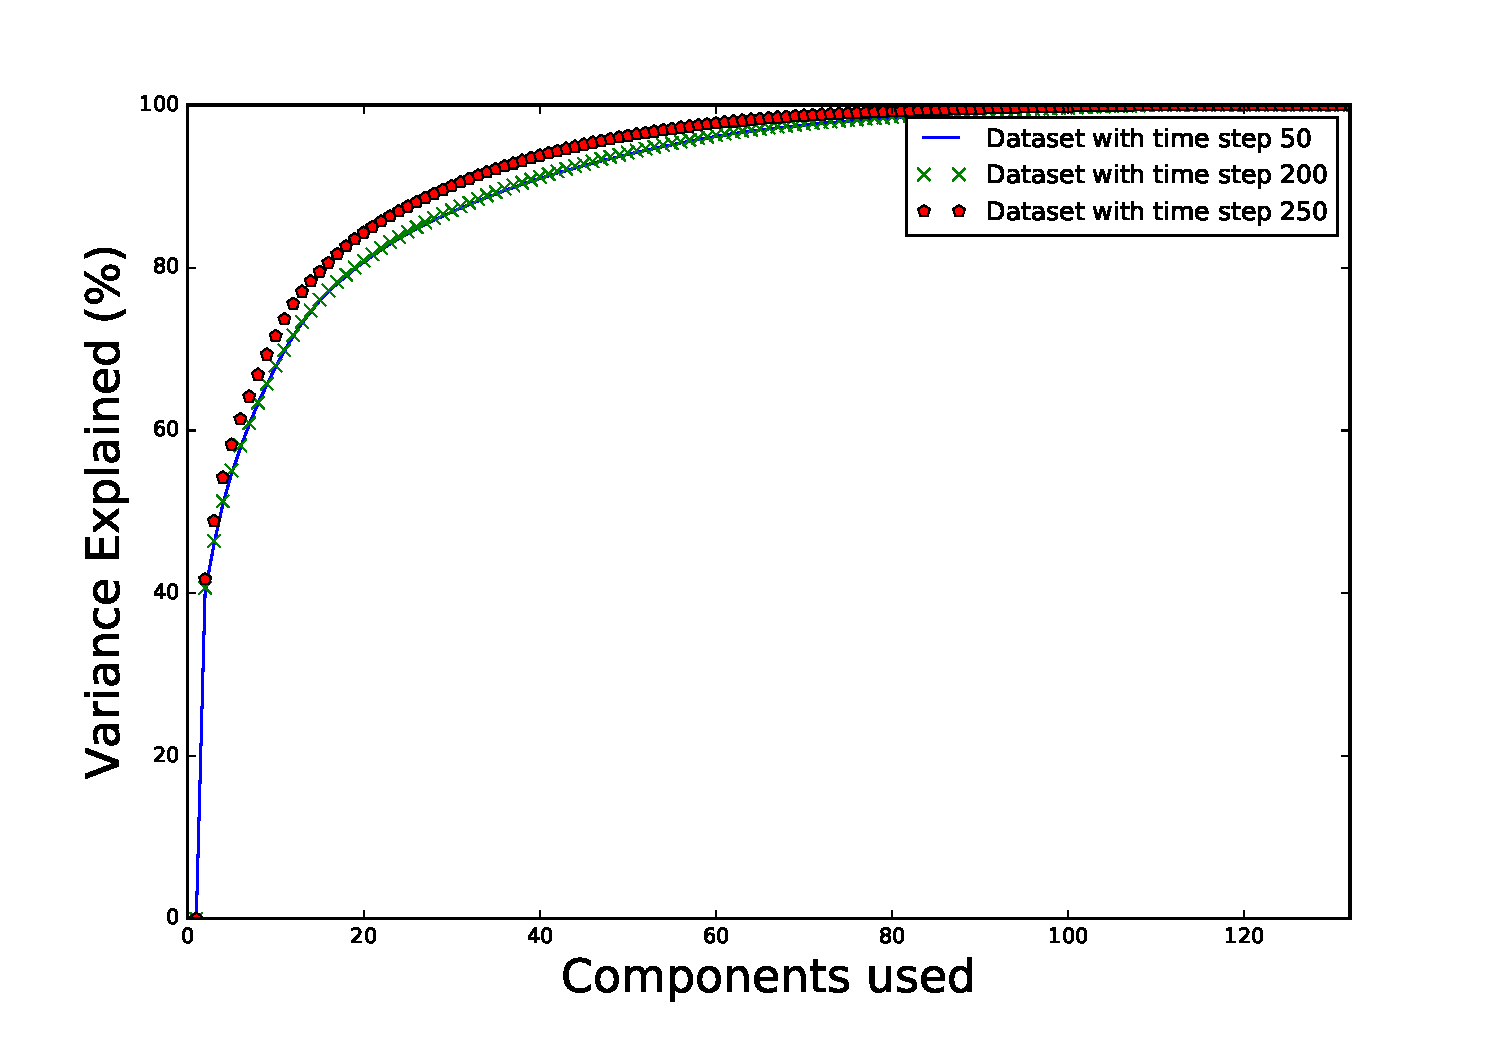
\includegraphics[width=0.55\linewidth]{figures/variance_explained_with_pca.pdf}
  \caption{Principle Component Analysis conducted on the three datasets reveals that the overall variance of the data can be maintained by using only a subset of the edges of the graph rather than all of them. The dataset with a time step of 250 ms needs less components to explain the variance than the other two, while the datasets with 200 and 50 ms time steps showed an almost exact level of variance explained with the number of components. This suggests that the 250 ms dataset is not complex enough, which might indicate that 2000 ms is too big of a time frame to record the granular communication speed of the brain.}
  \label{fig:pca_analysis_variance}
\end{figure}

\begin{table}[H]
\centering
\caption{Different component numbers are needed for each dataset to maintain a certain level of variance explained using PCA for dimensionality reduction. These values for components required for reaching a score standard were used to produce reduced forms of the datasets as noted in table \ref{tab:pca_datasets}. These reduced forms of the datasets were then analyzed in figure \ref{fig:silhouette_scores}.}
\label{tab:components_needed_for_variance}
\begin{tabular}{|c|c|c|c|}
\hline
 &  80\% variance explained &  90\% variance explained & 99\% variance explained \\ \hline
 
 Components in dataset 50 & 20 &  38&  87  \\ \hline
 Components in dataset 200 & 20 &  37&  87\\ \hline
 Components in dataset 250 & 16 &  30&  76  \\ \hline
\end{tabular}
\end{table}



\subsubsection{Clustering}
Once the dimensionality of the data was reduced with PCA, a Gaussian Mixture clusterer was initiated for each dataset from table \ref{tab:pca_datasets}, and all number of clusters from $2$ to $40$ were tried and tested by the Silhouette Coefficient and Calinsky-Harabaz Index scorers (Figs. \ref{fig:silhouette_scores}, \ref{fig:calinsky_scores}).

The complete ordered list of procedures was:
\begin{itemize}
  \item Removing NaN's with 0's if any exist in the edge weights
  \item Splitting the dataset into three datasets depending on the time step used
  \item Vectorizing the graphs so that each graph is a data point
  \item Running PCA analysis on the three datasets with varying degree of variance kept, creating 9 total datasets
  \item Clustering the PCA-reduced datasets with cluster numbers from 2 to 40.
  \item Computing Silhouette and Calinsky scores on the clusters in the previous step
\end{itemize}

The procedures were implemented successfully, but computing the silhouette and Calinsky scores was a bottleneck as it required calculating the distances between each data point. This could possibly have been avoided by pre-calculating the distances between all data points and passing them to the silhouette and Calinsky scoring functions, a feature available in the sci-kit learn library.

\begin{figure}[H]
  \centering
  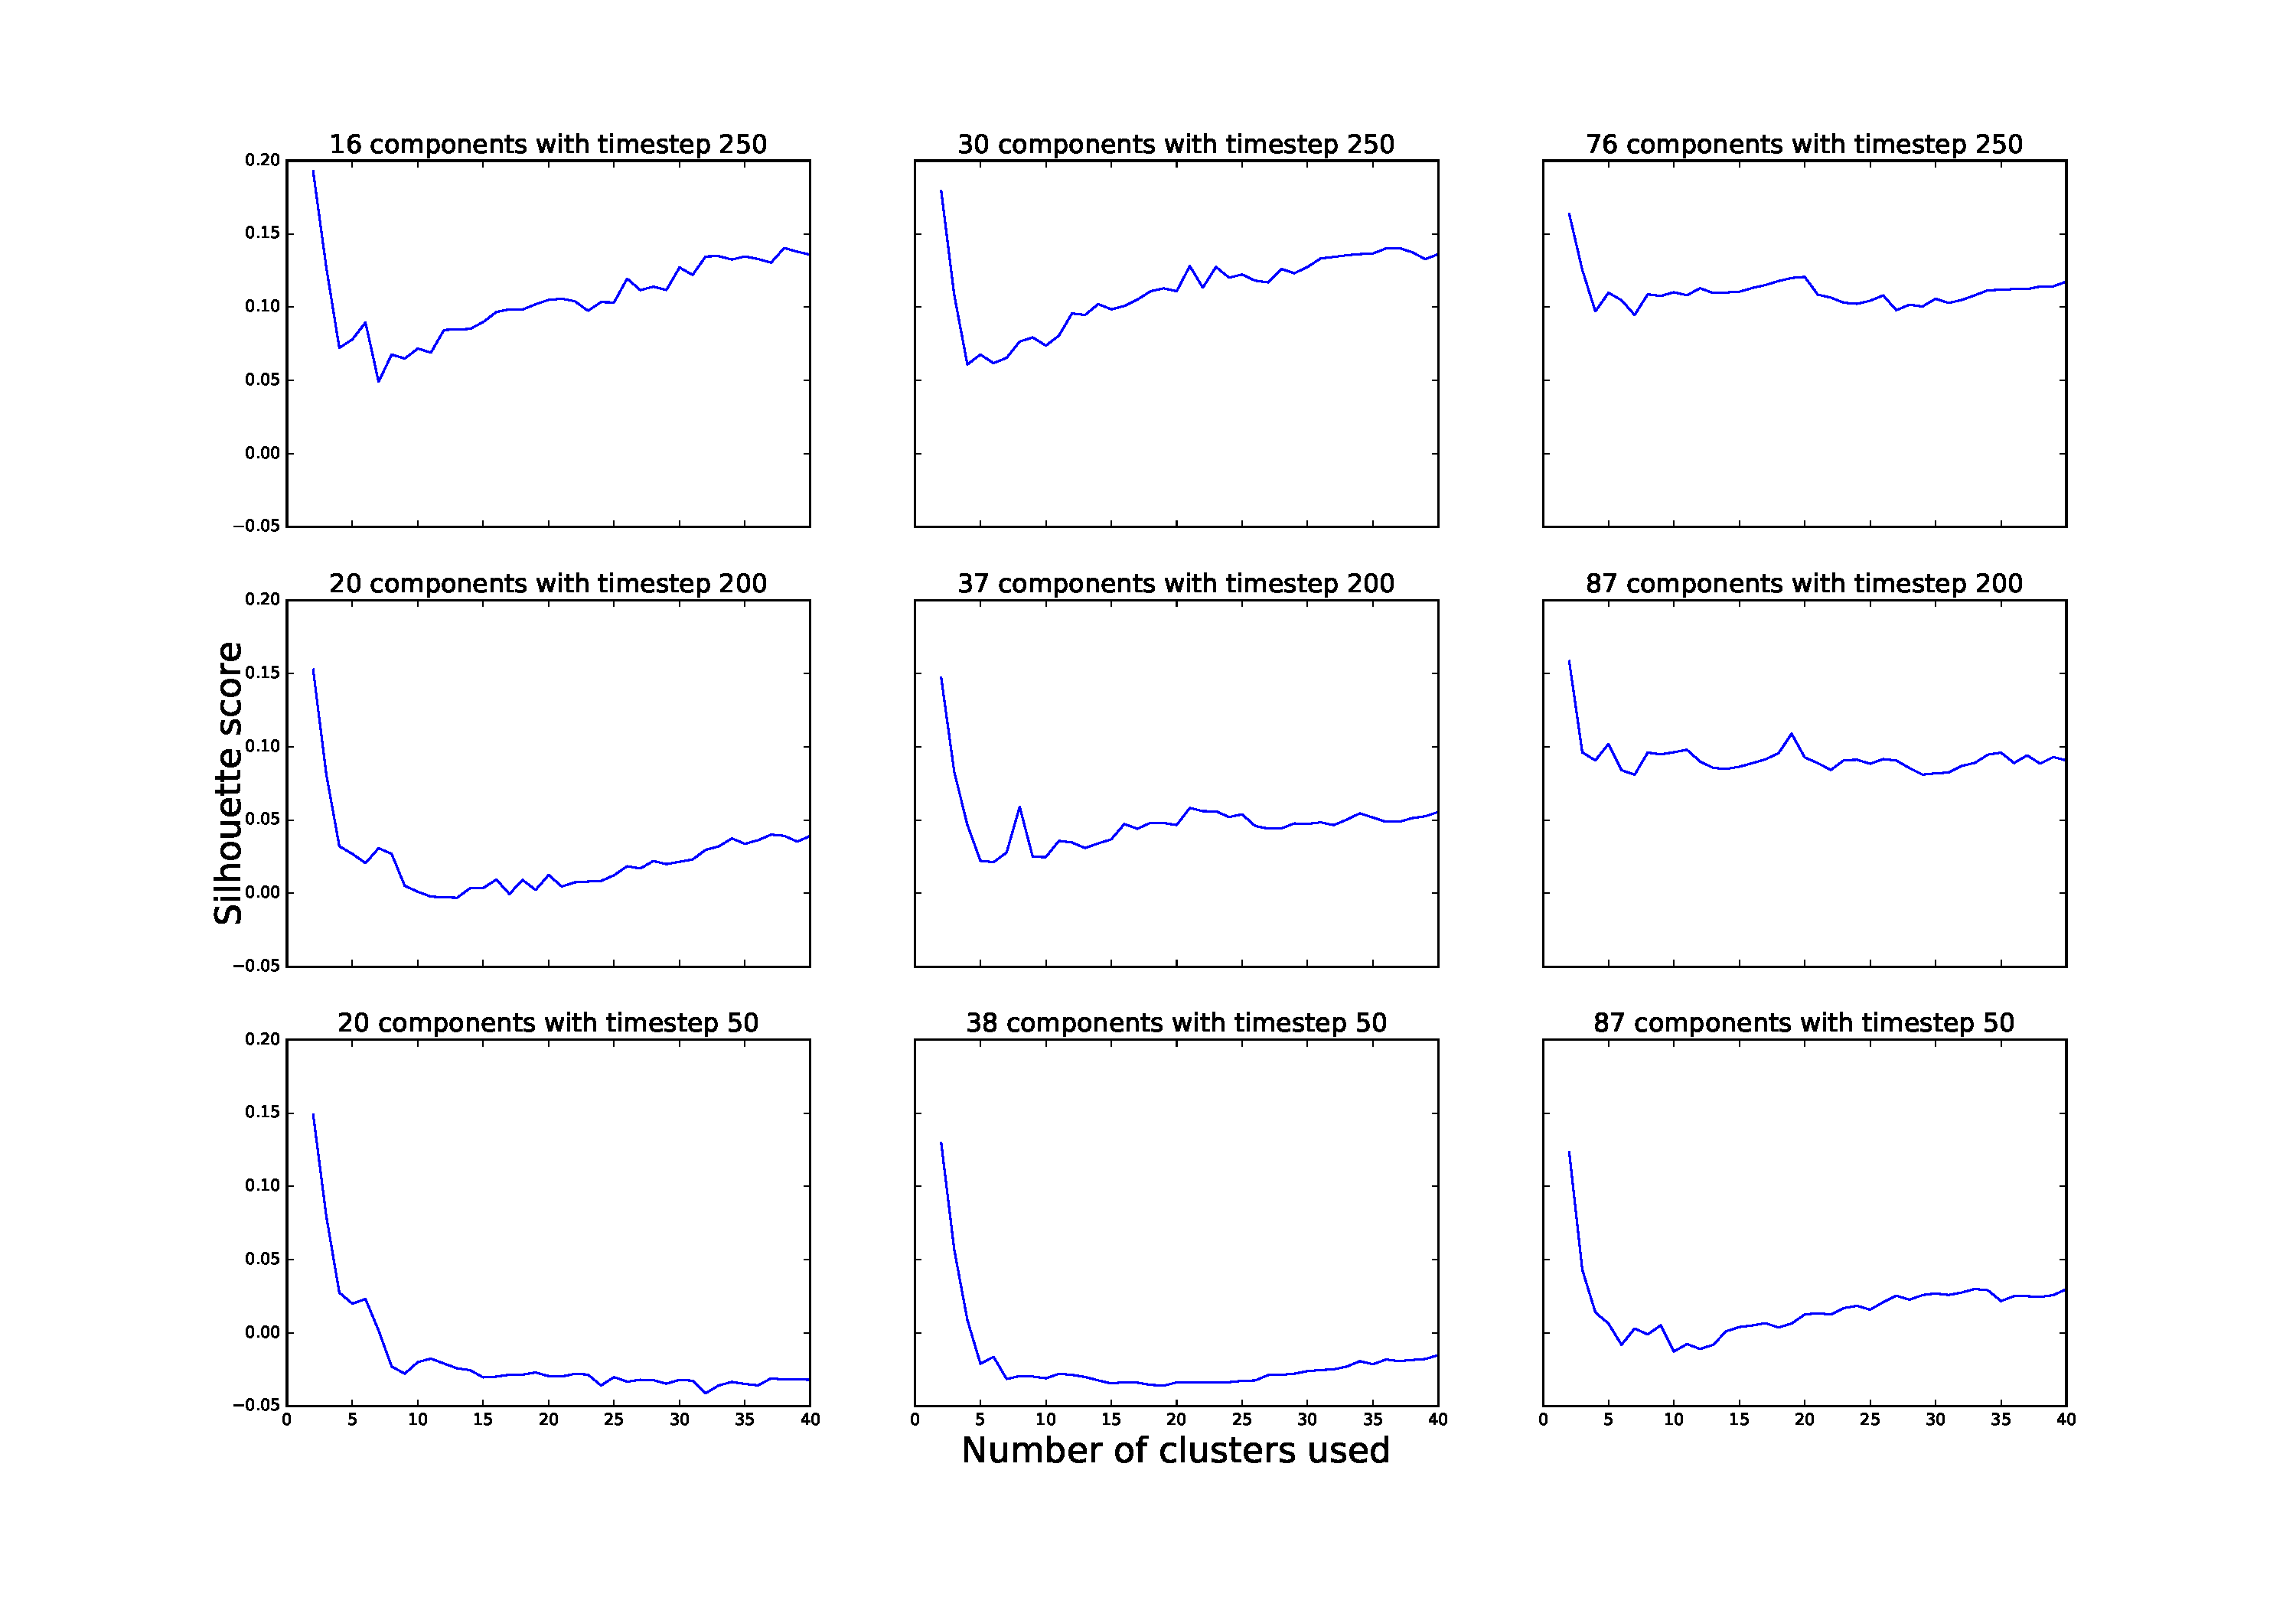
\includegraphics[width=\linewidth]{figures/silhouette_scores.pdf}
  \caption{Silhouette scores for clustering with different cluster numbers. Scores close to 1 suggest clusters that are dense and well separated; scores close to -1 suggest clusters that overlap and are not dense. The best score is consistently when there are only two clusters, and dips greatly when creating more clusters but begins to rise after ~30 clusters. With the dataset 250 and dataset 50, PCA with less components (16 and 20 components respectively) showed a better silhouette score than the other, higher component reduced datasets. However, dataset 200 showed a better silhouette score when more components were used. Especially with a rather thin margin of difference in scores between components, it is difficult to conclude whether having more PCA reductionist approach is beneficial.}
  \label{fig:silhouette_scores}
\end{figure}



\begin{figure}[H]
  \centering
  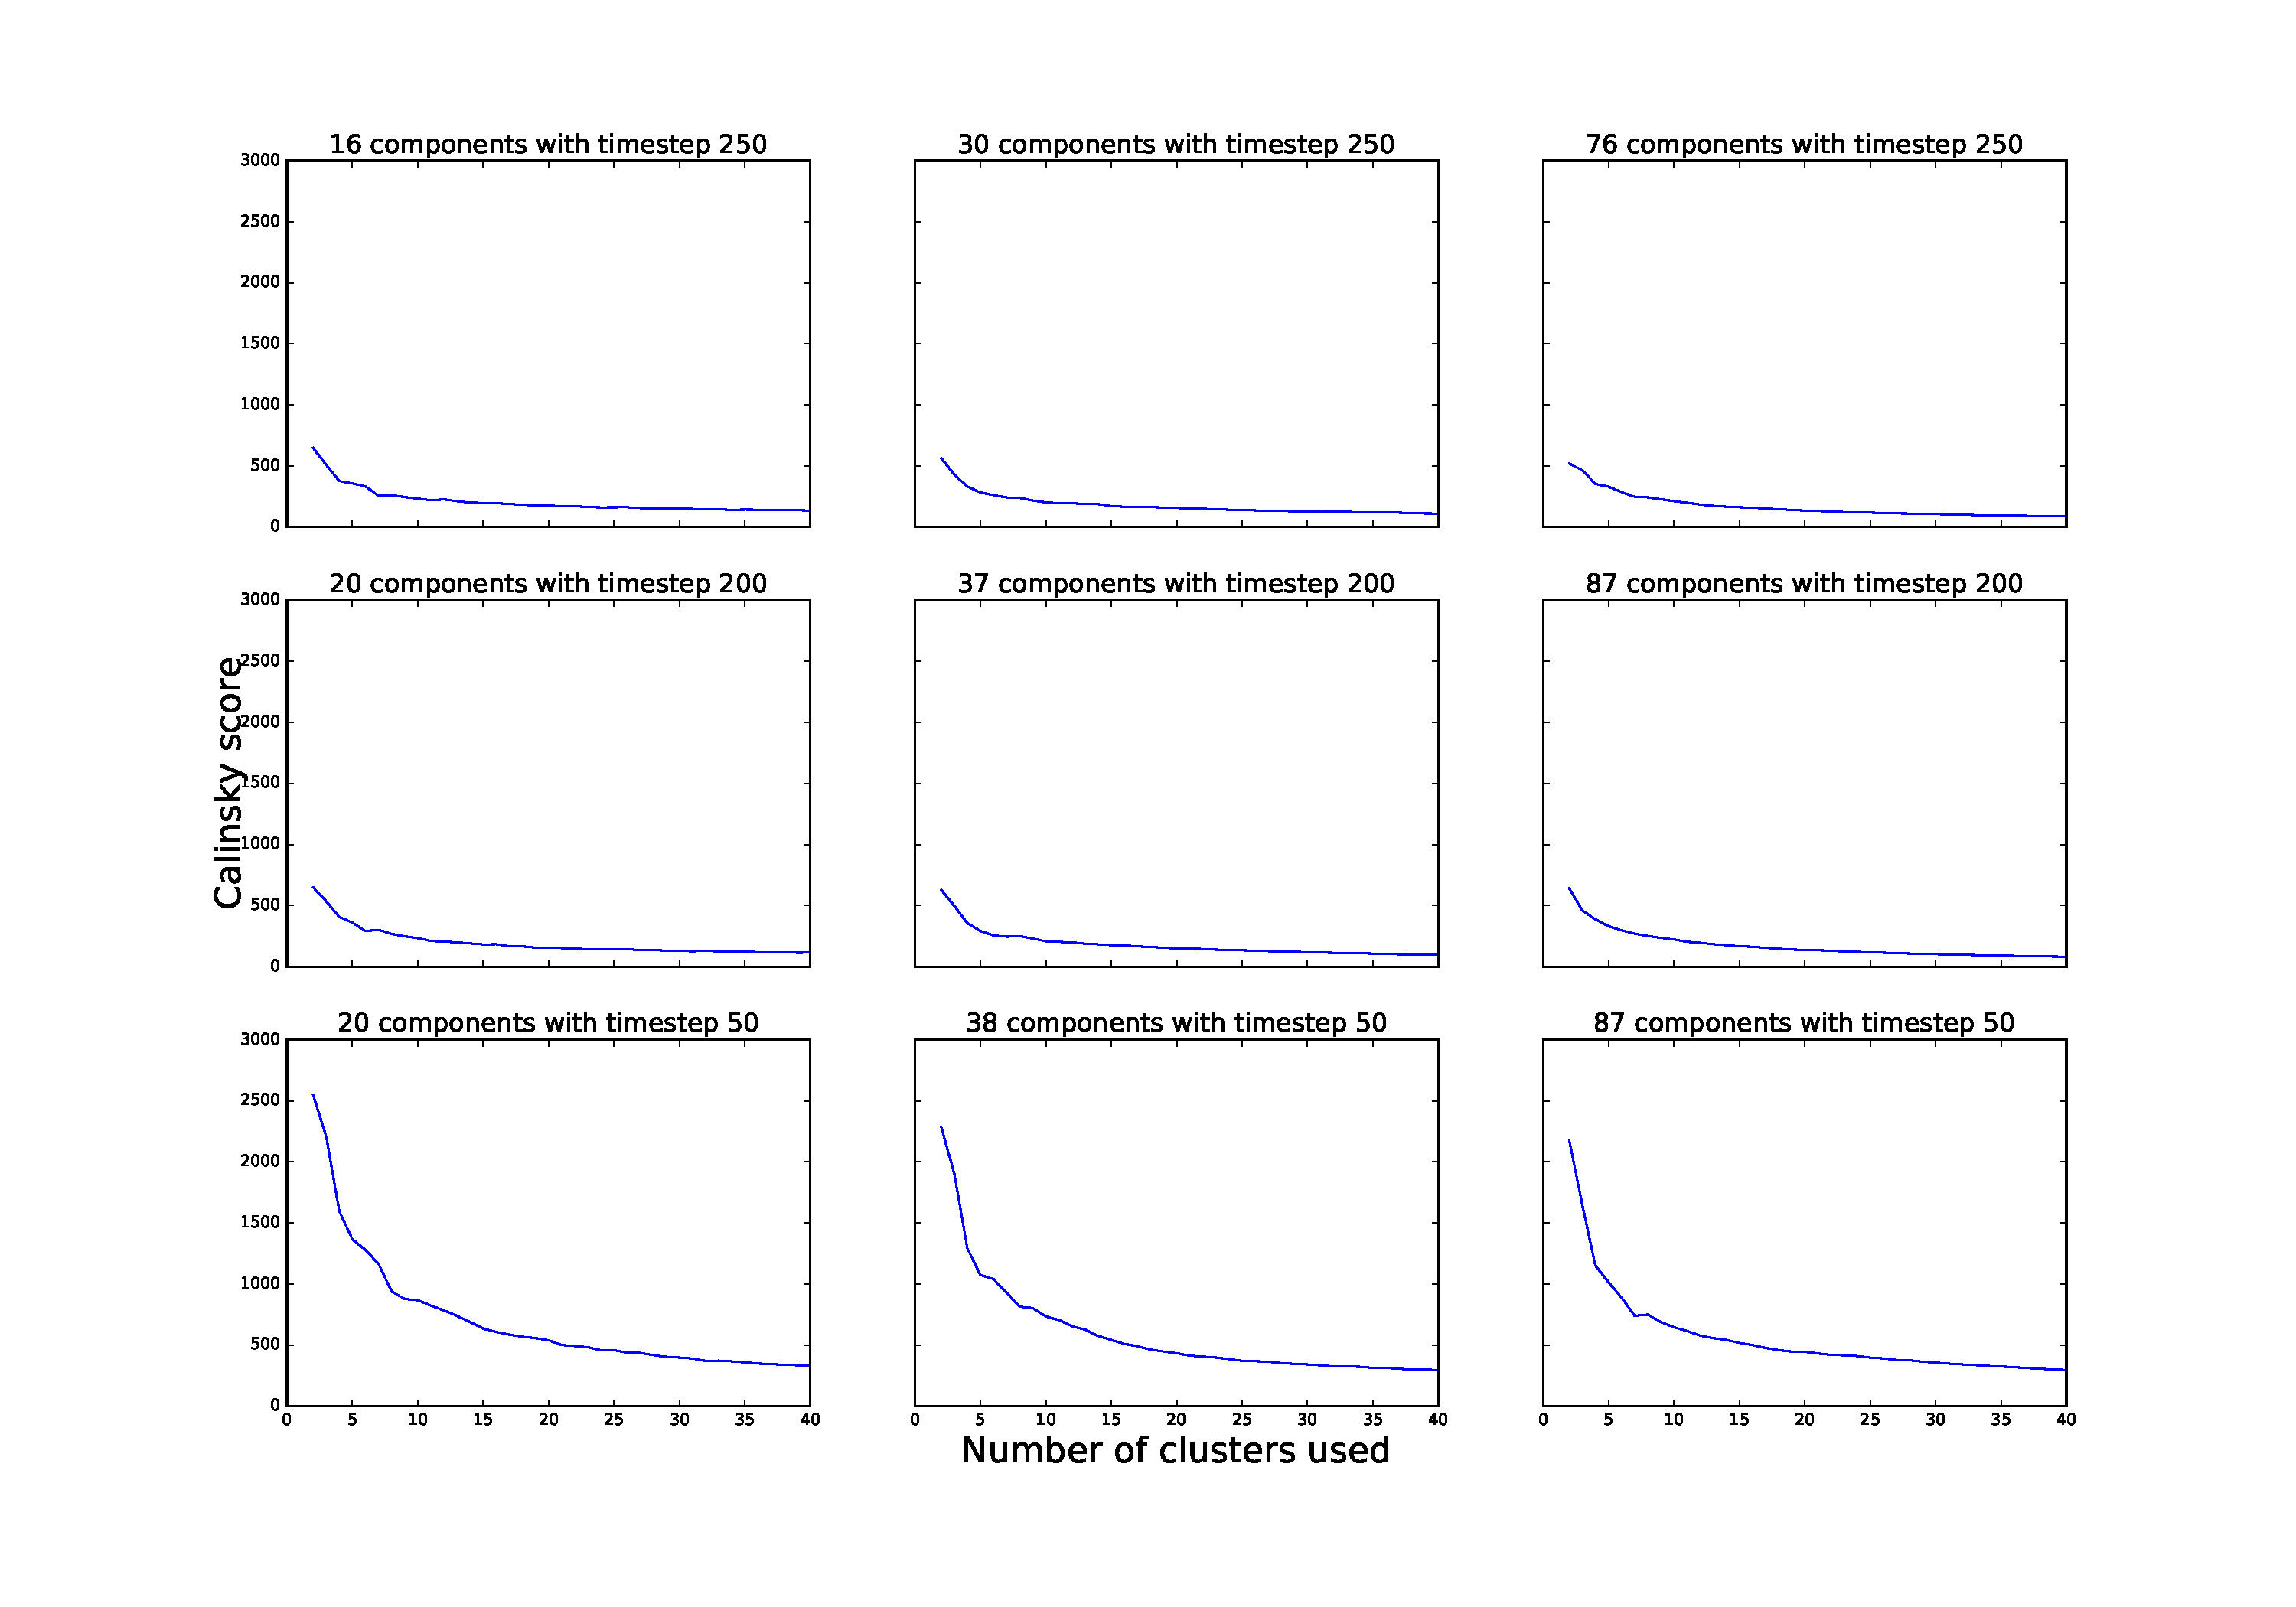
\includegraphics[width=\linewidth]{figures/calinsky_scores.pdf}
  \caption{Calinsky-Harabaz scores for clustering with different cluster numbers. Higher scores mean more separated and dense clusters, which is positive. The score dips greatly when creating more than two clusters, but begins to rise after ~30 clusters. The silhouette scores show that having more components when reducing with PCA results in better clustering scores. The scores also show that scores for the reduced data that keep 99\% of the variance (right column) are all similar in score and trend.}
  \label{fig:calinsky_scores}
\end{figure}

From figures \ref{fig:silhouette_scores} and \ref{fig:calinsky_scores}, it can be seen that the best clustering number is two, and it happens with dataset \textit{reduced 50 80} (dataset that is made with time step of 50 and transformed with PCA). We therefore fine tuned a Gaussian Mixture model with the \textit{reduced 50 80} dataset using Grid Search as implemented by the scikit learn library. The silhouette score was used as a scoring function for the grid search performance measurement. The parameters tuned with grid search was the \textit{covariance type} (with a choice of tied, diagonal, sphere, or full), and the best parameter was 'tied' with a silhouette score of $0.254$. This is an increase of 0.05 in the silhouette score, which is a ~25\% improvement.

\subsection{Results}

The results so far indicate that the rat's brain showed the presence of two distinct brain states, as we can cluster the brain's communication network into two clusters. This could be good news, since we can assume that the two brain states are \textit{epilepsy state} and \textit{normal state}. This simplifies our choice of metric to evaluate the model since we can use a simple F1 measurement by assuming the less frequent brain state is the epileptic state, and record the less occurring cluster as the epileptic cluster; we then test the time indicies of this cluster with the time indicies we were given for when epilepsy was evoked. Since we know that the epilepsy happened between seconds 447-457 and 250-260, we set true labels to be $0$ for all data points that were in that time period, and $1$ for all other data points. We then set the less frequent cluster to be of label $0$ (epilepsy cluster) and the more frequent cluster to $1$ (non-epilepsy cluster). Our evaluation metric then becomes the F1 score of the predicted labels against the true labels that we produced given the knowledge of our experiment.

Using the fine-tuned model, we achieve an F1 score of 0.788, which seems acceptable at first, but is rather disappointing when considering that the blind benchmark discussed in section \ref{sec:benchmark} has a score of 0.99. This is mainly due to the fact that the epilepsy state is infrequent, and so a clustering of non-epilepsy state as epilepsy creates a great error. This indicates that our model does not perform better than blindly guessing that there is only one state in the brain. This does not align with our hopes and expectations for the clustering solution. 

To analyze what our model is doing, we plot an annotated time strip that shows what each time window of causality was clustered to (Fig. \ref{fig:strip_visual}). From this graph, it can be seen that there is no correlation between what we observe in the real-life experiment and our clustering on the graph series constructed from Sugihara Causality measures. 

\begin{figure}[H]
  \centering
  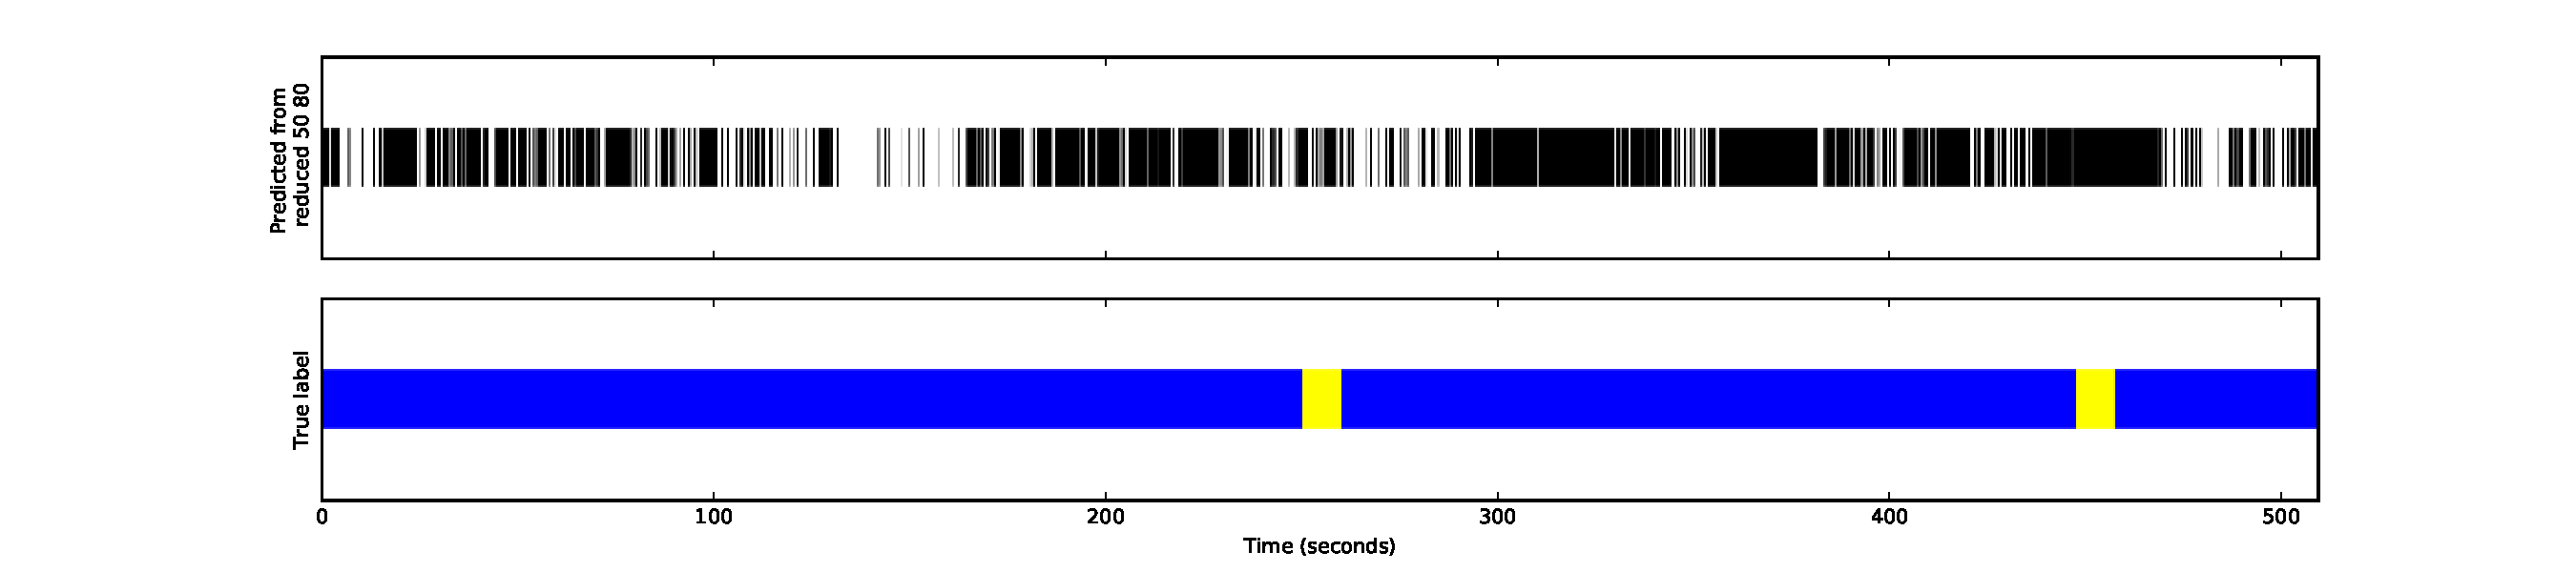
\includegraphics[width=\linewidth]{figures/strip_visual.pdf}
  \caption{Time strips that show the epilepsy time track and the results of the respective clustering done on the Sugihara Causality graphs from those time windows. Blue corresponds to true non-epileptic state; yellow to true epileptic state; white to predicted epileptic state; and black to predicted non-epileptic state. There are only two clusters in the top bar. The clustering results does not show any correlation with the actual epilepsy induction time series.}
  \label{fig:strip_visual}
\end{figure}


\subsection{Discussion}
Initial analysis shows that the causality network is very dense with highly weighted edges. The high density of the graph could have been a side effect of Sugihara's model ability to detect downstream causality. If that is the case, then many of the causal connections detected could in fact be residuals of upstream interactions in the brain network. Put in another way, if region A of the brain was causing region B to fire, and region B causes region C to fire, then the Sugihara causality model would report a causality measure between A and C. Downstream causality measures can be detected by observing both the magnitude of the cross map skill as well as the time lag that produces the greatest cross map skill (Fig. 3 in \cite{Ye2015}). Although we could have used this method in our experiment to remove the possibility of picking up extra weights from downstream causality, initial trials showed that the computational power required for that analysis were greater than the capacity available at UCCS. 

Concerning the high possibility of the presence of unidirectional forcing from figure \ref{fig:diff_within_pair_hist}, Ye \textit{et al.} showed unidirectional forcing can be untangled by inspecting the greatest time lag of the two that produces the highest causality measure (Fig. 2 in \cite{Ye2015}). In order to allay the problem of unidirectional forcing, the best lag of each pair is considered. This is a tricky problem because there is no clear range for which to test the lag. This is because the time delay for neuronal activity is yet studied, and how that translates to EEG data could be tricky. We reserve the use of this method due to its computational complexity which would add to the already high time complexity of the analysis.

The theoretical implications of this model could present a novel representation of information flow in the brain and determining causality within the brain. If the graph output of this method id reliable, it could help outline information flow within the brain, much like one would observe in a magnetic wave flowing through an fMRI recording. 



\subsection{Future Work}

Since various improvements can be made to this work, we break it down by stage of implementation.

\subsubsection{Methods}
It would have been enriching to our knowledge of our true labels if we had access to exactly what the rat was doing during the experiment. A video capture of the rat, or recorded structured interventions to the rat's behavior could have provided more opportunity to label the data with ground truth. For example, we could have shone light into the rat's eyes, and recorded that as a separate brain state; we could have put the rat on a hamster wheel and recorded his running as a separate brain state; eating food could be a brain state; and sleeping is another possible brain state. All these interventions to the rat's environment could enable us to gain more labels rather than the simple epilepsy, non-epilepsy labeling system we worked with. Although this complicates our approach, it would allow us access to better scoring metrics other than the silhouette and Calinksy-Harabaz scores, where the labels have to be known.

\subsubsection{Sugihara Causality Network}
Future work in this area could focus on verifying this model through controlled experiments. Such experiments could be in the form of stimulating a part of the brain (e.g. shining strong light on an the eye to excite the visual cortex) and observing the model's behavior. One would expect a high value of out degrees from the specific region during such an experiment, as it attempts to convey a considerable portion of information to the rest of the brain. Moreover, a clear proof should be presented as to what the most reliable time window and step size ought to be when producing the causality graphs. Such a task can be done by measuring graph similarity of the same time segment as the time window gets shortened incrementally.

\subsubsection{Data Processing}
Apart from collecting the data and applying Sugihara Causality on the dataset (which took 2 days), calculating the current source density using kCSD was by far the most time consuming process. Even though we do not discuss the details of how that was done in this project (we provide already processed kCSD data), it would have been nice to see a GPU implementation of the kCSD, which took advantage of CPU parallelism but not GPU parallelism. This would massively improve the speed of the implementation and allow for testing more various approaches in the Sugihara Causality step. 

\subsubsection{Cluster Scoring with Higher Dimensions}
Due to the high dimensionality of the dataset we worked with, it was difficult to visually measure how well the clustering with different number of clusters took place. Beyond three dimensions, it is impossible to visualize the dataset with labels, and although the PCA reduction resulted in a greatly reduced dimensional feature, it was not enough to allow us to visualize the clusters visually.
Following the assumption that downstream causality decreases in magnitude as it travels downstream in the network, we can use this to traverse the graph and rid of any paths that decreases in causality as it goes downstream.

\subsection{Conclusion}
The experiment we conduscted transformed 32 EEG electrode signals into 12 regional neuronal activity signals, and created a (theoretical) communication network from those signals using Sugihara Causality. These communication graphs were analyzed by unsupervised learning using the Gaussian Mixture model for the goal of gaining some insight into the epileptic state, and test whether unsupervised clustering is able to discriminate between brain states from the communication networks. From our initial results, it is clear that our approach is not successful in distinguishing brain states in a rat's brain. However, the ground work has been laid for future explorations in the topic of communication networks in the brain. 

\section{Conclusion}
The paper shows promising initial results using the Sugihara CCM model to construct causality graphs between brain regions. We find that the brain network for this experiment is highly causal with a range of time windows. This, however, could be due in part to experimental design limitations, where the electrodes were 1 mm apart which might have caused electrical interference. To to limit this phenomenon we used kCSD to preprocess the data. Initial results show a time varying graph in which information flow can be tracked. At the moment, more analysis is required to make a conclusions on the capabilities of the pairwise causality graph model. Some of most incurring difficulties to overcome are the running complexity of the kCSD preprocessing and CCM algorithm required for the analysis of the amount of pairs in a large network, and the mathematical representation of information flow within the time-dependent graph. We plan on using the Neuroclustering algorithm to discretize the EEG data into epileptic seizures, extract causal network features from the stages, and train a k-means learning algorithm on the created feature set. The implications of these findings could relate more generally to discoverability of causality in modeling scalable natural phenomena. Real world applications manifest in localization of epilepsy in the brain. Furthermore, if the technique of distinguishing causal networks in systems and clustering their properties is successful, it could be a clear indications that the Sugihara causality model is able to detect causation in extremely complex systems comparable to the human brain.

\section*{Acknowledgment}

Special thanks goes to Dr. Somogivari and Dorrottya R. from Winger RCP, Budapest for providing the neuronal data used in this paper. Furthermore, Dr. Peter Erdi is thanked for his patient guidance of this research topic which was instrumental for the production of this paper.

\balance
\bibliographystyle{IEEEtran}
\bibliography{IEEEabrv,main.bib}
\end{document}
